\documentclass[11pt]{article}%
\usepackage{geometry}%
\geometry{a4paper,
  lmargin=2cm,rmargin=2cm,tmargin=2.5cm,bmargin=2.5cm}

\usepackage{array}
\usepackage{paralist}

\usepackage[svgnames, usenames, dvipsnames]{xcolor}
\xdefinecolor{RecColor}{named}{Aqua}
\xdefinecolor{IncColor}{named}{Aqua}
\xdefinecolor{ImpColor}{named}{PaleGreen}

% \usepackage{frcursive}

\usepackage{adjustbox}

%%%%%%%%%%%
\newcommand{\cRB}[1]{{\color{Red} \pmb{#1}}} %
\newcommand{\cR}[1]{{\color{Red} {#1}}} %
\newcommand{\cBB}[1]{{\color{Blue} \pmb{#1}}}
\newcommand{\cB}[1]{{\color{Blue} {#1}}}
\newcommand{\cGB}[1]{{\color{LimeGreen} \pmb{#1}}}
\newcommand{\cG}[1]{{\color{LimeGreen} {#1}}}

%%%%%%%%%%

\usepackage{diagbox} %
\usepackage{colortbl} %
\usepackage{multirow} %
\usepackage{pgf} %
\usepackage{environ} %
\usepackage{fancybox} %
\usepackage{textcomp} %
\usepackage{marvosym} %

%%%%%%%%%% pour qu'une cellcolor ne recouvre pas le trait du tableau
\usepackage{hhline}%

\usepackage{pgfplots}
\pgfplotsset{compat=1.10}
\usepgfplotslibrary{patchplots}
\usepgfplotslibrary{fillbetween}
\usepackage{tikz,tkz-tab}
\usepackage{ifthen}
\usepackage{calc}
\usetikzlibrary{calc,decorations.pathreplacing,arrows,positioning} 
\usetikzlibrary{fit,shapes,backgrounds}
\usepackage[nomessages]{fp}% http://ctan.org/pkg/fp

\usetikzlibrary{matrix,arrows,decorations.pathmorphing,
  decorations.pathreplacing} 

\newcommand{\myunit}{1 cm}
\tikzset{
    node style sp/.style={draw,circle,minimum size=\myunit},
    node style ge/.style={circle,minimum size=\myunit},
    arrow style mul/.style={draw,sloped,midway,fill=white},
    arrow style plus/.style={midway,sloped,fill=white},
}

%%%%%%%%%%%%%%
%%%%% écrire des inférieur égal ou supérieur égal avec typographie
%%%%% francaise
%%%%%%%%%%%%%

\renewcommand{\geq}{\geqslant}
\renewcommand{\leq}{\leqslant}
\renewcommand{\emptyset}{\varnothing}

\newcommand{\Leq}{\leqslant}
\newcommand{\Geq}{\geqslant}

%%%%%%%%%%%%%%
%%%%% Macro Celia
%%%%%%%%%%%%%

\newcommand{\ff}[2]{\left[#1, #2\right]} %
\newcommand{\fo}[2]{\left[#1, #2\right[} %
\newcommand{\of}[2]{\left]#1, #2\right]} %
\newcommand{\soo}[2]{\left]#1, #2\right[} %
\newcommand{\abs}[1]{\left|#1\right|} %
\newcommand{\Ent}[1]{\left\lfloor #1 \right\rfloor} %


%%%%%%%%%%%%%%
%%%%% tikz : comment dessiner un "oeil"
%%%%%%%%%%%%%

\newcommand{\eye}[4]% size, x, y, rotation
{ \draw[rotate around={#4:(#2,#3)}] (#2,#3) -- ++(-.5*55:#1) (#2,#3)
  -- ++(.5*55:#1); \draw (#2,#3) ++(#4+55:.75*#1) arc
  (#4+55:#4-55:.75*#1);
  % IRIS
  \draw[fill=gray] (#2,#3) ++(#4+55/3:.75*#1) arc
  (#4+180-55:#4+180+55:.28*#1);
  % PUPIL, a filled arc
  \draw[fill=black] (#2,#3) ++(#4+55/3:.75*#1) arc
  (#4+55/3:#4-55/3:.75*#1);%
}


%%%%%%%%%%
%% discontinuité fonction
\newcommand\pointg[2]{%
  \draw[color = red, very thick] (#1+0.15, #2-.04)--(#1, #2-.04)--(#1,
  #2+.04)--(#1+0.15, #2+.04);%
}%

\newcommand\pointd[2]{%
  \draw[color = red, very thick] (#1-0.15, #2+.04)--(#1, #2+.04)--(#1,
  #2-.04)--(#1-0.15, #2-.04);%
}%

%%%%%%%%%%
%%% 1 : position abscisse, 2 : position ordonnée, 3 : taille, 4 : couleur
%%%%%%%%%%
% \newcommand\pointG[4]{%
%   \draw[color = #4, very thick] (#1+#3, #2-(#3/3.75))--(#1,
%   #2-(#3/3.75))--(#1, #2+(#3/3.75))--(#1+#3, #2+(#3/3.75)) %
% }%

\newcommand\pointG[4]{%
  \draw[color = #4, very thick] ({#1+#3/3.75}, {#2-#3})--(#1,
  {#2-#3})--(#1, {#2+#3})--({#1+#3/3.75}, {#2+#3}) %
}%

\newcommand\pointD[4]{%
  \draw[color = #4, very thick] ({#1-#3/3.75}, {#2+#3})--(#1,
  {#2+#3})--(#1, {#2-#3})--({#1-#3/3.75}, {#2-#3}) %
}%

\newcommand\spointG[4]{%
  \draw[color = #4, very thick] ({#1+#3/1.75}, {#2-#3})--(#1,
  {#2-#3})--(#1, {#2+#3})--({#1+#3/1.75}, {#2+#3}) %
}%

\newcommand\spointD[4]{%
  \draw[color = #4, very thick] ({#1-#3/2}, {#2+#3})--(#1,
  {#2+#3})--(#1, {#2-#3})--({#1-#3/2}, {#2-#3}) %
}%

%%%%%%%%%%

\newcommand{\Pb}{\mathtt{P}}

%%%%%%%%%%%%%%%
%%% Pour citer un précédent item
%%%%%%%%%%%%%%%
\newcommand{\itbf}[1]{{\small \bf \textit{#1}}}


%%%%%%%%%%%%%%%
%%% Quelques couleurs
%%%%%%%%%%%%%%%

\xdefinecolor{cancelcolor}{named}{Red}
\xdefinecolor{intI}{named}{ProcessBlue}
\xdefinecolor{intJ}{named}{ForestGreen}

%%%%%%%%%%%%%%%
%%%%%%%%%%%%%%%
% barrer du texte
\usetikzlibrary{shapes.misc}

\makeatletter
% \definecolor{cancelcolor}{rgb}{0.127,0.372,0.987}
\newcommand{\tikz@bcancel}[1]{%
  \begin{tikzpicture}[baseline=(textbox.base), inner sep=0pt]
    \node[strike out, draw] (textbox) {#1}[thick, color=cancelcolor];
    \useasboundingbox (textbox);
  \end{tikzpicture}%
}
\newcommand{\bcancel}[1]{%
  \relax\ifmmode
    \mathchoice{\tikz@bcancel{$\displaystyle#1$}}
               {\tikz@bcancel{$\textstyle#1$}}
               {\tikz@bcancel{$\scriptstyle#1$}}
               {\tikz@bcancel{$\scriptscriptstyle#1$}}
  \else
    \tikz@bcancel{\strut#1}%
  \fi
}
\newcommand{\tikz@xcancel}[1]{%
  \begin{tikzpicture}[baseline=(textbox.base),inner sep=0pt]
  \node[cross out,draw] (textbox) {#1}[thick, color=cancelcolor];
  \useasboundingbox (textbox);
  \end{tikzpicture}%
}
\newcommand{\xcancel}[1]{%
  \relax\ifmmode
    \mathchoice{\tikz@xcancel{$\displaystyle#1$}}
               {\tikz@xcancel{$\textstyle#1$}}
               {\tikz@xcancel{$\scriptstyle#1$}}
               {\tikz@xcancel{$\scriptscriptstyle#1$}}
  \else
    \tikz@xcancel{\strut#1}%
  \fi
}
\makeatother

\newcommand{\xcancelRA}{\xcancel{\rule[-.15cm]{0cm}{.5cm} \Rightarrow
    \rule[-.15cm]{0cm}{.5cm}}}

%%%%%%%%%%%%%%%%%%%%%%%%%%%%%%%%%%%
%%%%%%%%%%%%%%%%%%%%%%%%%%%%%%%%%%%

\newcommand{\vide}{\multicolumn{1}{c}{}}

%%%%%%%%%%%%%%%%%%%%%%%%%%%%%%%%%%%
%%%%%%%%%%%%%%%%%%%%%%%%%%%%%%%%%%%


\usepackage{multicol}
% \usepackage[latin1]{inputenc}
% \usepackage[T1]{fontenc}
\usepackage[utf8]{inputenc}
\usepackage[T1]{fontenc}
\usepackage[normalem]{ulem}
\usepackage[french]{babel}

\usepackage{url}    
\usepackage{hyperref}
\hypersetup{
  backref=true,
  pagebackref=true,
  hyperindex=true,
  colorlinks=true,
  breaklinks=true,
  urlcolor=blue,
  linkcolor=black,
  %%%%%%%%
  % ATTENTION : red changé en black pour le Livre !
  %%%%%%%%
  bookmarks=true,
  bookmarksopen=true
}

%%%%%%%%%%%%%%%%%%%%%%%%%%%%%%%%%%%%%%%%%%%
%% Pour faire des traits diagonaux dans les tableaux
%% Nécessite slashbox.sty
%\usepackage{slashbox}

\usepackage{tipa}
\usepackage{verbatim,listings}
\usepackage{graphicx}
\usepackage{fancyhdr}
\usepackage{mathrsfs}
\usepackage{pifont}
\usepackage{tablists}
\usepackage{dsfont,amsfonts,amssymb,amsmath,amsthm,stmaryrd,upgreek,manfnt}
\usepackage{enumerate}

%\newcolumntype{M}[1]{p{#1}}
\newcolumntype{C}[1]{>{\centering}m{#1}}
\newcolumntype{R}[1]{>{\raggedright}m{#1}}
\newcolumntype{L}[1]{>{\raggedleft}m{#1}}
\newcolumntype{P}[1]{>{\raggedright}p{#1}}
\newcolumntype{B}[1]{>{\raggedright}b{#1}}
\newcolumntype{Q}[1]{>{\raggedright}t{#1}}

\newcommand{\alias}[2]{
\providecommand{#1}{}
\renewcommand{#1}{#2}
}
\alias{\R}{\mathbb{R}}
\alias{\N}{\mathbb{N}}
\alias{\Z}{\mathbb{Z}}
\alias{\Q}{\mathbb{Q}}
\alias{\C}{\mathbb{C}}
\alias{\K}{\mathbb{K}}

%%%%%%%%%%%%
%% rendre +infty et -infty plus petits
%%%%%%%%%%%%
\newcommand{\sinfty}{{\scriptstyle \infty}}

%%%%%%%%%%%%%%%%%%%%%%%%%%%%%%%
%%%%% macros TP Scilab %%%%%%%%
\newcommand{\Scilab}{\textbf{Scilab}} %
\newcommand{\Scinotes}{\textbf{SciNotes}} %
\newcommand{\faire}{\noindent $\blacktriangleright$ } %
\newcommand{\fitem}{\scalebox{.8}{$\blacktriangleright$}} %
\newcommand{\entree}{{\small\texttt{ENTRÉE}}} %
\newcommand{\tab}{{\small\texttt{TAB}}} %
\newcommand{\mt}[1]{\mathtt{#1}} %
% guillemets droits

\newcommand{\ttq}{\textquotesingle} %

\newcommand{\reponse}[1]{\longboxed{
    \begin{array}{C{0.9\textwidth}}
      \nl[#1]
    \end{array}
  }} %

\newcommand{\reponseR}[1]{\longboxed{
    \begin{array}{R{0.9\textwidth}}
      #1
    \end{array}
  }} %

\newcommand{\reponseC}[1]{\longboxed{
    \begin{array}{C{0.9\textwidth}}
      #1
    \end{array}
  }} %

\colorlet{pyfunction}{Blue}
\colorlet{pyCle}{Magenta}
\colorlet{pycomment}{LimeGreen}
\colorlet{pydoc}{Cyan}
% \colorlet{SansCo}{white}
% \colorlet{AvecCo}{black}

\newcommand{\visible}[1]{{\color{ASCo}\colorlet{pydoc}{pyDo}\colorlet{pycomment}{pyCo}\colorlet{pyfunction}{pyF}\colorlet{pyCle}{pyC}\colorlet{function}{sciFun}\colorlet{var}{sciVar}\colorlet{if}{sciIf}\colorlet{comment}{sciComment}#1}} %

%%%% à changer ????
\newcommand{\invisible}[1]{{\color{ASCo}\colorlet{pydoc}{pyDo}\colorlet{pycomment}{pyCo}\colorlet{pyfunction}{pyF}\colorlet{pyCle}{pyC}\colorlet{function}{sciFun}\colorlet{var}{sciVar}\colorlet{if}{sciIf}\colorlet{comment}{sciComment}#1}} %

\newcommand{\invisibleCol}[2]{{\color{#1}#2}} %

\NewEnviron{solution} %
{ %
  \Boxed{
    \begin{array}{>{\color{ASCo}} R{0.9\textwidth}}
      \colorlet{pycomment}{pyCo}
      \colorlet{pydoc}{pyDo}
      \colorlet{pyfunction}{pyF}
      \colorlet{pyCle}{pyC}
      \colorlet{function}{sciFun}
      \colorlet{var}{sciVar}
      \colorlet{if}{sciIf}
      \colorlet{comment}{sciComment}
      \BODY
    \end{array}
  } %
} %

\NewEnviron{solutionC} %
{ %
  \Boxed{
    \begin{array}{>{\color{ASCo}} C{0.9\textwidth}}
      \colorlet{pycomment}{pyCo}
      \colorlet{pydoc}{pyDo}
      \colorlet{pyfunction}{pyF}
      \colorlet{pyCle}{pyC}
      \colorlet{function}{sciFun}
      \colorlet{var}{sciVar}
      \colorlet{if}{sciIf}
      \colorlet{comment}{sciComment}
      \BODY
    \end{array}
  } %
} %

\newcommand{\invite}{--\!\!>} %

%%%%% nouvel environnement tabular pour retour console %%%%
\colorlet{ConsoleColor}{Black!12}
\colorlet{function}{Red}
\colorlet{var}{Maroon}
\colorlet{if}{Magenta}
\colorlet{comment}{LimeGreen}

\newcommand{\tcVar}[1]{\textcolor{var}{\bf \small #1}} %
\newcommand{\tcFun}[1]{\textcolor{function}{#1}} %
\newcommand{\tcIf}[1]{\textcolor{if}{#1}} %
\newcommand{\tcFor}[1]{\textcolor{if}{#1}} %

\newcommand{\moins}{\!\!\!\!\!\!- }
\newcommand{\espn}{\!\!\!\!\!\!}

\usepackage{booktabs,varwidth} \newsavebox\TBox
\newenvironment{console}
{\begin{lrbox}{\TBox}\varwidth{\linewidth}
    \tabular{>{\tt\small}R{0.84\textwidth}}
    \nl[-.4cm]} {\endtabular\endvarwidth\end{lrbox}%
  \fboxsep=1pt\colorbox{ConsoleColor}{\usebox\TBox}}

\newcommand{\lInv}[1]{%
  $\invite$ #1} %

\newcommand{\lAns}[1]{%
  \qquad ans \ = \nl %
  \qquad \qquad #1} %

\newcommand{\lVar}[2]{%
  \qquad #1 \ = \nl %
  \qquad \qquad #2} %

\newcommand{\lDisp}[1]{%
  #1 %
} %

\newcommand{\ligne}[1]{\underline{\small \tt #1}} %

\newcommand{\ligneAns}[2]{%
  $\invite$ #1 \nl %
  \qquad ans \ = \nl %
  \qquad \qquad #2} %

\newcommand{\ligneVar}[3]{%
  $\invite$ #1 \nl %
  \qquad #2 \ = \nl %
  \qquad \qquad #3} %

\newcommand{\ligneErr}[3]{%
  $\invite$ #1 \nl %
  \quad !-{-}error #2 \nl %
  #3} %
%%%%%%%%%%%%%%%%%%%%%% 

\newcommand{\bs}[1]{\boldsymbol{#1}} %
\newcommand{\nll}{\nl[.4cm]} %
\newcommand{\nle}{\nl[.2cm]} %
%% opérateur puissance copiant l'affichage Scilab
%\newcommand{\puis}{\!\!\!~^{\scriptscriptstyle\pmb{\wedge}}}
\newcommand{\puis}{\mbox{$\hspace{-.1cm}~^{\scriptscriptstyle\pmb{\wedge}}
    \hspace{0.05cm}$}} %
\newcommand{\pointpuis}{.\mbox{$\hspace{-.15cm}~^{\scriptscriptstyle\pmb{\wedge}}$}} %
\newcommand{\Sfois}{\mbox{$\mt{\star}$}} %

%%%%% nouvel environnement tabular pour les encadrés Scilab %%%%
\newenvironment{encadre}
{\begin{lrbox}{\TBox}\varwidth{\linewidth}
    \tabular{>{\tt\small}C{0.1\textwidth}>{\small}R{0.7\textwidth}}}
  {\endtabular\endvarwidth\end{lrbox}%
  \fboxsep=1pt\longboxed{\usebox\TBox}}

\newenvironment{encadreL}
{\begin{lrbox}{\TBox}\varwidth{\linewidth}
    \tabular{>{\tt\small}C{0.25\textwidth}>{\small}R{0.6\textwidth}}}
  {\endtabular\endvarwidth\end{lrbox}%
  \fboxsep=1pt\longboxed{\usebox\TBox}}

\newenvironment{encadreF}
{\begin{lrbox}{\TBox}\varwidth{\linewidth}
    \tabular{>{\tt\small}C{0.2\textwidth}>{\small}R{0.70\textwidth}}}
  {\endtabular\endvarwidth\end{lrbox}%
  \fboxsep=1pt\longboxed{\usebox\TBox}}

\newenvironment{encadreLL}[2]
{\begin{lrbox}{\TBox}\varwidth{\linewidth}
    \tabular{>{\tt\small}C{#1\textwidth}>{\small}R{#2\textwidth}}}
  {\endtabular\endvarwidth\end{lrbox}%
  \fboxsep=1pt\longboxed{\usebox\TBox}}

%%%%% nouvel environnement tabular pour les script et fonctions %%%%
\newcommand{\commentaireDL}[1]{\multicolumn{1}{l}{\it
    \textcolor{comment}{$\slash\slash$ #1}}}

\newcommand{\commentaire}[1]{{\textcolor{comment}{$\slash\slash$ #1}}}

\newcounter{cptcol}

\newcommand{\nocount}{\multicolumn{1}{c}{}}

\newcommand{\sciNo}[1]{{\small \underbar #1}}

\NewEnviron{scilab}{ %
  \setcounter{cptcol}{0}
  \begin{center}
    \longboxed{
      \begin{tabular}{>{\stepcounter{cptcol}{\tiny \underbar
              \thecptcol}}c>{\tt}l}
        \BODY
      \end{tabular}
    }
  \end{center}
}

\NewEnviron{scilabNC}{ %
  \begin{center}
    \longboxed{
      \begin{tabular}{>{\tt}l} %
          \BODY
      \end{tabular}
    }
  \end{center}
}

\NewEnviron{scilabC}[1]{ %
  \setcounter{cptcol}{#1}
  \begin{center}
    \longboxed{
      \begin{tabular}{>{\stepcounter{cptcol}{\tiny \underbar
              \thecptcol}}c>{\tt}l}
        \BODY
      \end{tabular}
    }
  \end{center}
}

\newcommand{\scisol}[1]{ %
  \setcounter{cptcol}{0}
  \longboxed{
    \begin{tabular}{>{\stepcounter{cptcol}{\tiny \underbar
            \thecptcol}}c>{\tt}l}
      #1
    \end{tabular}
  }
}

\newcommand{\scisolNC}[1]{ %
  \longboxed{
    \begin{tabular}{>{\tt}l}
      #1
    \end{tabular}
  }
}

\newcommand{\scisolC}[2]{ %
  \setcounter{cptcol}{#1}
  \longboxed{
    \begin{tabular}{>{\stepcounter{cptcol}{\tiny \underbar
            \thecptcol}}c>{\tt}l}
      #2
    \end{tabular}
  }
}

\NewEnviron{syntaxe}{ %
  % \fcolorbox{black}{Yellow!20}{\setlength{\fboxsep}{3mm}
  \shadowbox{
    \setlength{\fboxsep}{3mm}
    \begin{tabular}{>{\tt}l}
      \BODY
    \end{tabular}
  }
}

%%%%% fin macros TP Scilab %%%%%%%%
%%%%%%%%%%%%%%%%%%%%%%%%%%%%%%%%%%%

%%%%%%%%%%%%%%%%%%%%%%%%%%%%%%%%%%%
%%%%% TP Python - listings %%%%%%%%
%%%%%%%%%%%%%%%%%%%%%%%%%%%%%%%%%%%
\newcommand{\Python}{\textbf{Python}} %

\lstset{% general command to set parameter(s)
basicstyle=\ttfamily\small, % print whole listing small
keywordstyle=\color{blue}\bfseries\underbar,
%% underlined bold black keywords
frame=lines,
xleftmargin=10mm,
numbers=left,
numberstyle=\tiny\underbar,
numbersep=10pt,
%identifierstyle=, % nothing happens
commentstyle=\color{green}, % white comments
%%stringstyle=\ttfamily, % typewriter type for strings
showstringspaces=false}

\newcommand{\pysolCpt}[2]{
  \setcounter{cptcol}{#1}
  \longboxed{
    \begin{tabular}{>{\stepcounter{cptcol}{\tiny \underbar
            \thecptcol}}c>{\tt}l}
        #2
      \end{tabular}
    }
} %

\newcommand{\pysol}[1]{
  \setcounter{cptcol}{0}
  \longboxed{
    \begin{tabular}{>{\stepcounter{cptcol}{\tiny \underbar
            \thecptcol}}c>{\tt}l}
        #1
      \end{tabular}
    }
} %

% \usepackage[labelsep=endash]{caption}

% avec un caption
\NewEnviron{pythonCap}[1]{ %
  \renewcommand{\tablename}{Programme}
  \setcounter{cptcol}{0}
  \begin{center}
    \longboxed{
      \begin{tabular}{>{\stepcounter{cptcol}{\tiny \underbar
              \thecptcol}}c>{\tt}l}
        \BODY
      \end{tabular}
    }
    \captionof{table}{#1}
  \end{center}
}

\NewEnviron{python}{ %
  \setcounter{cptcol}{0}
  \begin{center}
    \longboxed{
      \begin{tabular}{>{\stepcounter{cptcol}{\tiny \underbar
              \thecptcol}}c>{\tt}l}
        \BODY
      \end{tabular}
    }
  \end{center}
}

\newcommand{\pyVar}[1]{\textcolor{var}{\bf \small #1}} %
\newcommand{\pyFun}[1]{\textcolor{pyfunction}{#1}} %
\newcommand{\pyCle}[1]{\textcolor{pyCle}{#1}} %
\newcommand{\pyImp}[1]{{\bf #1}} %

%%%%% commentaire python %%%%
\newcommand{\pyComDL}[1]{\multicolumn{1}{l}{\textcolor{pycomment}{\#
      #1}}}

\newcommand{\pyCom}[1]{{\textcolor{pycomment}{\# #1}}}
\newcommand{\pyDoc}[1]{{\textcolor{pydoc}{#1}}}

\newcommand{\pyNo}[1]{{\small \underbar #1}}

%%%%%%%%%%%%%%%%%%%%%%%%%%%%%%%%%%%
%%%%%% Système linéaire paramétré : écrire les opérations au-dessus
%%%%%% d'un symbole équivalent
%%%%%%%%%%%%%%%%%%%%%%%%%%%%%%%%%%%

\usepackage{systeme}

\NewEnviron{arrayEq}{ %
  \stackrel{\scalebox{.6}{$
      \begin{array}{l} 
        \BODY \\[.1cm]
      \end{array}$}
  }{\Longleftrightarrow}
}

\NewEnviron{arrayEg}{ %
  \stackrel{\scalebox{.6}{$
      \begin{array}{l} 
        \BODY \\[.1cm]
      \end{array}$}
  }{=}
}

\NewEnviron{operationEq}{ %
  \scalebox{.6}{$
    \begin{array}{l} 
      \scalebox{1.6}{$\mbox{Opérations :}$} \\[.2cm]
      \BODY \\[.1cm]
    \end{array}$}
}

% \NewEnviron{arraySys}[1]{ %
%   \sysdelim\{.\systeme[#1]{ %
%     \BODY %
%   } %
% }

%%%%%

%%%%%%%%%%
%%%%%%%%%% ESSAI
\newlength\fboxseph
\newlength\fboxsepva
\newlength\fboxsepvb

\setlength\fboxsepva{0.2cm}
\setlength\fboxsepvb{0.2cm}
\setlength\fboxseph{0.2cm}

\makeatletter

\def\longboxed#1{\leavevmode\setbox\@tempboxa\hbox{\color@begingroup%
\kern\fboxseph{\m@th$\displaystyle #1 $}\kern\fboxseph%
\color@endgroup }\my@frameb@x\relax}

\def\my@frameb@x#1{%
  \@tempdima\fboxrule \advance\@tempdima \fboxsepva \advance\@tempdima
  \dp\@tempboxa\hbox {%
    \lower \@tempdima \hbox {%
      \vbox {\hrule\@height\fboxrule \hbox{\vrule\@width\fboxrule #1
          \vbox{%
            \vskip\fboxsepva \box\@tempboxa \vskip\fboxsepvb}#1
          \vrule\@width\fboxrule }%
        \hrule \@height \fboxrule }}}}

\newcommand{\boxedhv}[3]{\setlength\fboxseph{#1cm}
  \setlength\fboxsepva{#2cm}\setlength\fboxsepvb{#2cm}\longboxed{#3}}

\newcommand{\boxedhvv}[4]{\setlength\fboxseph{#1cm}
  \setlength\fboxsepva{#2cm}\setlength\fboxsepvb{#3cm}\longboxed{#4}}

\newcommand{\Boxed}[1]{{\setlength\fboxseph{0.2cm}
  \setlength\fboxsepva{0.2cm}\setlength\fboxsepvb{0.2cm}\longboxed{#1}}}

\newcommand{\mBoxed}[1]{{\setlength\fboxseph{0.2cm}
  \setlength\fboxsepva{0.2cm}\setlength\fboxsepvb{0.2cm}\longboxed{\mbox{#1}}}}

\newcommand{\mboxed}[1]{{\setlength\fboxseph{0.2cm}
  \setlength\fboxsepva{0.2cm}\setlength\fboxsepvb{0.2cm}\boxed{\mbox{#1}}}}

\newsavebox{\fmbox}
\newenvironment{fmpage}[1]
     {\begin{lrbox}{\fmbox}\begin{minipage}{#1}}
     {\end{minipage}\end{lrbox}\fbox{\usebox{\fmbox}}}

%%%%%%%%%%
%%%%%%%%%%

\DeclareMathOperator{\ch}{ch}
\DeclareMathOperator{\sh}{sh}

%%%%%%%%%%
%%%%%%%%%%

\newcommand{\norme}[1]{\Vert #1 \Vert}

%\newcommand*\widefbox[1]{\fbox{\hspace{2em}#1\hspace{2em}}}

\newcommand{\nl}{\tabularnewline}

\newcommand{\hand}{\noindent\ding{43}\ }
\newcommand{\ie}{\textit{i.e. }}
\newcommand{\cf}{\textit{cf }}

\newcommand{\Card}{\operatorname{Card}}

\newcommand{\aire}{\mathcal{A}}

\newcommand{\LL}[1]{\mathscr{L}(#1)} %
\newcommand{\B}{\mathscr{B}} %
\newcommand{\Bc}[1]{B_{#1}} %
\newcommand{\M}[1]{\mathscr{M}_{#1}(\mathbb{R})}

\DeclareMathOperator{\im}{Im}
\DeclareMathOperator{\kr}{Ker}
\DeclareMathOperator{\rg}{rg}
\DeclareMathOperator{\spc}{Sp}
\DeclareMathOperator{\sgn}{sgn}
\DeclareMathOperator{\supp}{Supp}

\newcommand{\Mat}{{\rm{Mat}}}
\newcommand{\Vect}[1]{{\rm{Vect}}\left(#1\right)}

\newenvironment{smatrix}{%
  \begin{adjustbox}{width=.9\width}
    $
    \begin{pmatrix}
    }{%      
    \end{pmatrix}
    $
  \end{adjustbox}
}

\newenvironment{sarray}[1]{%
  \begin{adjustbox}{width=.9\width}
    $
    \begin{array}{#1}
    }{%      
    \end{array}
    $
  \end{adjustbox}
}

\newcommand{\vd}[2]{
  \scalebox{.8}{
    $\left(\!
      \begin{array}{c}
        #1 \\
        #2
      \end{array}
    \!\right)$
    }}

\newcommand{\vt}[3]{
  \scalebox{.8}{
    $\left(\!
      \begin{array}{c}
        #1 \\
        #2 \\
        #3 
      \end{array}
    \!\right)$
    }}

\newcommand{\vq}[4]{
  \scalebox{.8}{
    $\left(\!
      \begin{array}{c}
        #1 \\
        #2 \\
        #3 \\
        #4 
      \end{array}
    \!\right)$
    }}

\newcommand{\vc}[5]{
  \scalebox{.8}{
    $\left(\!
      \begin{array}{c}
        #1 \\
        #2 \\
        #3 \\
        #4 \\
        #5 
      \end{array}
    \!\right)$
    }}

\newcommand{\ee}{\text{e}}

\newcommand{\dd}{\text{d}}

%%% Ensemble de définition
\newcommand{\Df}{\mathscr{D}}
\newcommand{\Cf}{\mathscr{C}}
\newcommand{\Ef}{\mathscr{C}}

\newcommand{\rond}[1]{\,\overset{\scriptscriptstyle \circ}{\!#1}}

\newcommand{\df}[2]{\dfrac{\partial #1}{\partial #2}} %
\newcommand{\dfn}[2]{\partial_{#2}(#1)} %
\newcommand{\ddfn}[2]{\partial^2_{#2}(#1)} %
\newcommand{\ddf}[2]{\dfrac{\partial^2 #1}{\partial #2^2}} %
\newcommand{\ddfr}[3]{\dfrac{\partial^2 #1}{\partial #2 \partial
    #3}} %


\newcommand{\dlim}[1]{{\displaystyle \lim_{#1} \ }}
\newcommand{\dlimPlus}[2]{
  \dlim{
    \scalebox{.6}{
      $
      \begin{array}{l}
        #1 \rightarrow #2\\
        #1 > #2
      \end{array}
      $}}}
\newcommand{\dlimMoins}[2]{
  \dlim{
    \scalebox{.6}{
      $
      \begin{array}{l}
        #1 \rightarrow #2\\
        #1 < #2
      \end{array}
      $}}}

%%%%%%%%%%%%%%
%% petit o, développement limité
%%%%%%%%%%%%%%

\newcommand{\oo}[2]{{\underset {{\overset {#1\rightarrow #2}{}}}{o}}} %
\newcommand{\oox}[1]{{\underset {{\overset {x\rightarrow #1}{}}}{o}}} %
\newcommand{\oon}{{\underset {{\overset {n\rightarrow +\infty}{}}}{o}}} %
\newcommand{\po}[1]{{\underset {{\overset {#1}{}}}{o}}} %
\newcommand{\neqx}[1]{{\ \underset {{\overset {x \to #1}{}}}{\not\sim}\ }} %
\newcommand{\eqx}[1]{{\ \underset {{\overset {x \to #1}{}}}{\sim}\ }} %
\newcommand{\eqn}{{\ \underset {{\overset {n \to +\infty}{}}}{\sim}\ }} %
\newcommand{\eq}[2]{{\ \underset {{\overset {#1 \to #2}{}}}{\sim}\ }} %
\newcommand{\DL}[1]{{\rm{DL}}_1 (#1)} %
\newcommand{\DLL}[1]{{\rm{DL}}_2 (#1)} %

\newcommand{\negl}{<<}

\newcommand{\neglP}[1]{\begin{array}{c}
    \vspace{-.2cm}\\
    << \\
    \vspace{-.7cm}\\
    {\scriptstyle #1}
  \end{array}}

%%%%%%%%%%%%%%
%% borne sup, inf, max, min
%%%%%%%%%%%%%%
\newcommand{\dsup}[1]{\displaystyle \sup_{#1} \ }
\newcommand{\dinf}[1]{\displaystyle \inf_{#1} \ }
\newcommand{\dmax}[1]{\max\limits_{#1} \ }
\newcommand{\dmin}[1]{\min\limits_{#1} \ }

\newcommand{\dcup}[2]{{\textstyle\bigcup\limits_{#1}^{#2}}\hspace{.1cm}}
%\displaystyle \bigcup_{#1}^{#2}}
\newcommand{\dcap}[2]{{\textstyle\bigcap\limits_{#1}^{#2}}\hspace{.1cm}}
% \displaystyle \bigcap_{#1}^{#2}
%%%%%%%%%%%%%%
%% opérateurs logiques
%%%%%%%%%%%%%%
\newcommand{\NON}[1]{\mathop{\small \tt{NON}} (#1)}
\newcommand{\ET}{\mathrel{\mathop{\small \mathtt{ET}}}}
\newcommand{\OU}{\mathrel{\mathop{\small \tt{OU}}}}
\newcommand{\XOR}{\mathrel{\mathop{\small \tt{XOR}}}}

\newcommand{\id}{{\rm{id}}}

\newcommand{\sbullet}{\scriptstyle \bullet}
\newcommand{\stimes}{\scriptstyle \times}

%%%%%%%%%%%%%%%%%%
%% Probabilités
%%%%%%%%%%%%%%%%%%
\newcommand{\Prob}{\mathbb{P}}
\newcommand{\Ev}[1]{\left[ {#1} \right]}
\newcommand{\Evmb}[1]{[ {#1} ]}
\newcommand{\E}{\mathbb{E}}
\newcommand{\V}{\mathbb{V}}
\newcommand{\Cov}{{\rm{Cov}}}
\newcommand{\U}[2]{\mathcal{U}(\llb #1, #2\rrb)}
\newcommand{\Uc}[2]{\mathcal{U}([#1, #2])}
\newcommand{\Ucof}[2]{\mathcal{U}(]#1, #2])}
\newcommand{\Ucoo}[2]{\mathcal{U}(]#1, #2[)}
\newcommand{\Ucfo}[2]{\mathcal{U}([#1, #2[)}
\newcommand{\Bern}[1]{\mathcal{B}\left(#1\right)}
\newcommand{\Bin}[2]{\mathcal{B}\left(#1, #2\right)}
\newcommand{\G}[1]{\mathcal{G}\left(#1\right)}
\newcommand{\Pois}[1]{\mathcal{P}\left(#1\right)}
\newcommand{\HG}[3]{\mathcal{H}\left(#1, #2, #3\right)}
\newcommand{\Exp}[1]{\mathcal{E}\left(#1\right)}
\newcommand{\Norm}[2]{\mathcal{N}\left(#1, #2\right)}

\DeclareMathOperator{\cov}{Cov}

\newcommand{\var}{v.a.r. }
\newcommand{\suit}{\hookrightarrow}

\newcommand{\flecheR}[1]{\rotatebox{90}{\scalebox{#1}{\color{red}
      $\curvearrowleft$}}}


\newcommand{\partie}[1]{\mathcal{P}(#1)}
\newcommand{\Cont}[1]{\mathcal{C}^{#1}}
\newcommand{\Contm}[1]{\mathcal{C}^{#1}_m}

\newcommand{\llb}{\llbracket}
\newcommand{\rrb}{\rrbracket}

%\newcommand{\im}[1]{{\rm{Im}}(#1)}
\newcommand{\imrec}[1]{#1^{- \mathds{1}}}

\newcommand{\unq}{\mathds{1}}

\newcommand{\Hyp}{\mathtt{H}}

\newcommand{\eme}[1]{#1^{\scriptsize \mbox{ème}}}
\newcommand{\er}[1]{#1^{\scriptsize \mbox{er}}}
\newcommand{\ere}[1]{#1^{\scriptsize \mbox{ère}}}
\newcommand{\nd}[1]{#1^{\scriptsize \mbox{nd}}}
\newcommand{\nde}[1]{#1^{\scriptsize \mbox{nde}}}

\newcommand{\truc}{\mathop{\top}}
\newcommand{\fois}{\mathop{\ast}}

\newcommand{\f}[1]{\overrightarrow{#1}}

\newcommand{\checked}{\textcolor{green}{\checkmark}}

\def\restriction#1#2{\mathchoice
              {\setbox1\hbox{${\displaystyle #1}_{\scriptstyle #2}$}
              \restrictionaux{#1}{#2}}
              {\setbox1\hbox{${\textstyle #1}_{\scriptstyle #2}$}
              \restrictionaux{#1}{#2}}
              {\setbox1\hbox{${\scriptstyle #1}_{\scriptscriptstyle #2}$}
              \restrictionaux{#1}{#2}}
              {\setbox1\hbox{${\scriptscriptstyle #1}_{\scriptscriptstyle #2}$}
              \restrictionaux{#1}{#2}}}
\def\restrictionaux#1#2{{#1\,\smash{\vrule height .8\ht1 depth .85\dp1}}_{\,#2}}

\makeatletter
\newcommand*{\da@rightarrow}{\mathchar"0\hexnumber@\symAMSa 4B }
\newcommand*{\da@leftarrow}{\mathchar"0\hexnumber@\symAMSa 4C }
\newcommand*{\xdashrightarrow}[2][]{%
  \mathrel{%
    \mathpalette{\da@xarrow{#1}{#2}{}\da@rightarrow{\,}{}}{}%
  }%
}
\newcommand{\xdashleftarrow}[2][]{%
  \mathrel{%
    \mathpalette{\da@xarrow{#1}{#2}\da@leftarrow{}{}{\,}}{}%
  }%
}
\newcommand*{\da@xarrow}[7]{%
  % #1: below
  % #2: above
  % #3: arrow left
  % #4: arrow right
  % #5: space left 
  % #6: space right
  % #7: math style 
  \sbox0{$\ifx#7\scriptstyle\scriptscriptstyle\else\scriptstyle\fi#5#1#6\m@th$}%
  \sbox2{$\ifx#7\scriptstyle\scriptscriptstyle\else\scriptstyle\fi#5#2#6\m@th$}%
  \sbox4{$#7\dabar@\m@th$}%
  \dimen@=\wd0 %
  \ifdim\wd2 >\dimen@
    \dimen@=\wd2 %   
  \fi
  \count@=2 %
  \def\da@bars{\dabar@\dabar@}%
  \@whiledim\count@\wd4<\dimen@\do{%
    \advance\count@\@ne
    \expandafter\def\expandafter\da@bars\expandafter{%
      \da@bars
      \dabar@ 
    }%
  }%  
  \mathrel{#3}%
  \mathrel{%   
    \mathop{\da@bars}\limits
    \ifx\\#1\\%
    \else
      _{\copy0}%
    \fi
    \ifx\\#2\\%
    \else
      ^{\copy2}%
    \fi
  }%   
  \mathrel{#4}%
}
\makeatother



\newcount\depth

\newcount\depth
\newcount\totaldepth

\makeatletter
\newcommand{\labelsymbol}{%
      \ifnum\depth=0
        %
      \else
        \rlap{\,$\bullet$}%
      \fi
}

\newcommand*\bernoulliTree[1]{%
    \depth=#1\relax            
    \totaldepth=#1\relax
    \draw node(root)[bernoulli/root] {\labelsymbol}[grow=right] \draw@bernoulli@tree;
    \draw \label@bernoulli@tree{root};                                   
}                                                                        

\def\draw@bernoulli@tree{%
    \ifnum\depth>0 
      child[parent anchor=east] foreach \type/\label in {left child/$E$,right child/$S$} {%
          node[bernoulli/\type] {\label\strut\labelsymbol} \draw@bernoulli@tree
      }
      coordinate[bernoulli/increment] (dummy)
   \fi%
}

\def\label@bernoulli@tree#1{%
    \ifnum\depth>0
      ($(#1)!0.5!(#1-1)$) node[fill=white,bernoulli/decrement] {\tiny$p$}
      \label@bernoulli@tree{#1-1}
      ($(#1)!0.5!(#1-2)$) node[fill=white] {\tiny$q$}
      \label@bernoulli@tree{#1-2}
      coordinate[bernoulli/increment] (dummy)
   \fi%
}

\makeatother

\tikzset{bernoulli/.cd,
         root/.style={},
         decrement/.code=\global\advance\depth by-1\relax,
         increment/.code=\global\advance\depth by 1\relax,
         left child/.style={bernoulli/decrement},
         right child/.style={}}


\newcommand{\eps}{\varepsilon}

% \newcommand{\tendi}[1]{\xrightarrow[\footnotesize #1 \rightarrow
%   +\infty]{}}%

\newcommand{\tend}{\rightarrow}%
\newcommand{\tendn}{\underset{n\to +\infty}{\longrightarrow}} %
\newcommand{\ntendn}{\underset{n\to
    +\infty}{\not\hspace{-.15cm}\longrightarrow}} %
% \newcommand{\tendn}{\xrightarrow[\footnotesize n \rightarrow
%   +\infty]{}}%
\newcommand{\Tendx}[1]{\xrightarrow[\footnotesize x \rightarrow
  #1]{}}%
\newcommand{\tendx}[1]{\underset{x\to #1}{\longrightarrow}}%
\newcommand{\ntendx}[1]{\underset{x\to #1}{\not\!\!\longrightarrow}}%
\newcommand{\tendd}[2]{\underset{#1\to #2}{\longrightarrow}}%
% \newcommand{\tendd}[2]{\xrightarrow[\footnotesize #1 \rightarrow
%   #2]{}}%
\newcommand{\tendash}[1]{\xdashrightarrow[\footnotesize #1 \rightarrow
  +\infty]{}}%
\newcommand{\tendashx}[1]{\xdashrightarrow[\footnotesize x \rightarrow
  #1]{}}%
\newcommand{\tendb}[1]{\underset{#1 \to +\infty}{\longrightarrow}}%
\newcommand{\tendL}{\overset{\mathscr L}{\underset{n \to
      +\infty}{\longrightarrow}}}%
\newcommand{\tendP}{\overset{\Prob}{\underset{n \to
      +\infty}{\longrightarrow}}}%
\newcommand{\tenddL}[1]{\overset{\mathscr L}{\underset{#1 \to
      +\infty}{\longrightarrow}}}%

\NewEnviron{attention}{ %
  ~\\[-.2cm]\noindent
  \begin{minipage}{\linewidth}
  \setlength{\fboxsep}{3mm}%
  \ \ \dbend \ \ %
  \fbox{\parbox[t]{.88\linewidth}{\BODY}} %
  \end{minipage}\\
}

\NewEnviron{sattention}[1]{ %
  ~\\[-.2cm]\noindent
  \begin{minipage}{#1\linewidth}
  \setlength{\fboxsep}{3mm}%
  \ \ \dbend \ \ %
  \fbox{\parbox[t]{.88\linewidth}{\BODY}} %
  \end{minipage}\\
}

%%%%% OBSOLETE %%%%%%

% \newcommand{\attention}[1]{
%   \noindent
%   \begin{tabular}{@{}l|p{11.5cm}|}
%     \cline{2-2}
%     \vspace{-.2cm} 
%     & \nl
%     \dbend & #1 \nl
%     \cline{2-2}
%   \end{tabular}
% }

% \newcommand{\attentionv}[2]{
%   \noindent
%   \begin{tabular}{@{}l|p{11.5cm}|}
%     \cline{2-2}
%     \vspace{-.2cm} 
%     & \nl
%     \dbend & #2 \nl[#1 cm]
%     \cline{2-2}
%   \end{tabular}
% }

\newcommand{\explainvb}[2]{
  \noindent
  \begin{tabular}{@{}l|p{11.5cm}|}
    \cline{2-2}
    \vspace{-.2cm} 
    & \nl
    \hand & #2 \nl [#1 cm]
    \cline{2-2}
  \end{tabular}
}


% \noindent
% \begin{tabular}{@{}l|lp{11cm}|}
%   \cline{3-3} 
%   \multicolumn{1}{@{}l@{\dbend}}{} & & #1 \nl
%   \multicolumn{1}{l}{} & & \nl [-.8cm]
%   & & #2 \nl
%   \cline{2-3}
% \end{tabular}

% \newcommand{\attention}[1]{
%   \noindent
%   \begin{tabular}{@{}@{}cp{11cm}}
%     \dbend & #1 \nl
%   \end{tabular}
% }

\newcommand{\PP}[1]{\mathcal{P}(#1)}
\newcommand{\HH}[1]{\mathcal{H}(#1)}
\newcommand{\FF}[1]{\mathcal{F}(#1)}

\newcommand{\DSum}[2]{\displaystyle\sum\limits_{#1}^{#2}\hspace{.1cm}}
\newcommand{\Sum}[2]{{\textstyle\sum\limits_{#1}^{#2}}\hspace{.1cm}}
\newcommand{\Serie}{\textstyle\sum\hspace{.1cm}}
\newcommand{\Prod}[2]{\textstyle\prod\limits_{#1}^{#2}}

\newcommand{\Prim}[3]{\left[\ {#1} \ \right]_{\scriptscriptstyle
   \hspace{-.15cm} ~_{#2}\, }^ {\scriptscriptstyle \hspace{-.15cm} ~^{#3}\, }}

% \newcommand{\Prim}[3]{\left[\ {#1} \ \right]_{\scriptscriptstyle
%     \!\!~_{#2}}^ {\scriptscriptstyle \!\!~^{#3}}}

\newcommand{\dint}[2]{\displaystyle \int_{#1}^{#2}\ }
\newcommand{\Int}[2]{{\rm{Int}}_{\scriptscriptstyle #1, #2}}
\newcommand{\dt}{\ dt}
\newcommand{\dx}{\ dx}

\newcommand{\llpar}[1]{\left(\!\!\!
    \begin{array}{c}
      \rule{0pt}{#1}
    \end{array}
  \!\!\!\right.}

\newcommand{\rrpar}[1]{\left.\!\!\!
    \begin{array}{c}
      \rule{0pt}{#1}
    \end{array}
  \!\!\!\right)}

\newcommand{\llacc}[1]{\left\{\!\!\!
    \begin{array}{c}
      \rule{0pt}{#1}
    \end{array}
  \!\!\!\right.}

\newcommand{\rracc}[1]{\left.\!\!\!
    \begin{array}{c}
      \rule{0pt}{#1}
    \end{array}
  \!\!\!\right\}}

\newcommand{\ttacc}[1]{\mbox{\rotatebox{-90}{\hspace{-.7cm}$\llacc{#1}$}}}
\newcommand{\bbacc}[1]{\mbox{\rotatebox{90}{\hspace{-.5cm}$\llacc{#1}$}}}

\newcommand{\comp}[1]{\overline{#1}}%

\newcommand{\dcomp}[2]{\stackrel{\mbox{\ \ \----}{\scriptscriptstyle
      #2}}{#1}}%

% \newcommand{\Comp}[2]{\stackrel{\mbox{\ \
%       \-------}{\scriptscriptstyle #2}}{#1}}

% \newcommand{\dcomp}[2]{\stackrel{\mbox{\ \
%       \-------}{\scriptscriptstyle #2}}{#1}}

\newcommand{\A}{\mathscr{A}}

\newcommand{\conc}[1]{
  \begin{center}
    \fbox{
      \begin{tabular}{c}
        #1
      \end{tabular}
    }
  \end{center}
}

\newcommand{\concC}[1]{
  \begin{center}
    \fbox{
    \begin{tabular}{C{10cm}}
      \quad #1 \quad
    \end{tabular}
    }
  \end{center}
}

\newcommand{\concL}[2]{
  \begin{center}
    \fbox{
    \begin{tabular}{C{#2cm}}
      \quad #1 \quad
    \end{tabular}
    }
  \end{center}
}


% \newcommand{\lims}[2]{\prod\limits_{#1}^{#2}}

\newtheorem{theorem}{Théorème}[]
\newtheorem{lemma}{Lemme}[]
\newtheorem{proposition}{Proposition}[]
\newtheorem{corollary}{Corollaire}[]

% \newenvironment{proof}[1][Démonstration]{\begin{trivlist}
% \item[\hskip \labelsep {\bfseries #1}]}{\end{trivlist}}
\newenvironment{definition}[1][Définition]{\begin{trivlist}
\item[\hskip \labelsep {\bfseries #1}]}{\end{trivlist}}
\newenvironment{example}[1][Exemple]{\begin{trivlist}
\item[\hskip \labelsep {\bfseries #1}]}{\end{trivlist}}
\newenvironment{examples}[1][Exemples]{\begin{trivlist}
\item[\hskip \labelsep {\bfseries #1}]}{\end{trivlist}}
\newenvironment{notation}[1][Notation]{\begin{trivlist}
\item[\hskip \labelsep {\bfseries #1}]}{\end{trivlist}}
\newenvironment{propriete}[1][Propriété]{\begin{trivlist}
\item[\hskip \labelsep {\bfseries #1}]}{\end{trivlist}}
\newenvironment{proprietes}[1][Propriétés]{\begin{trivlist}
\item[\hskip \labelsep {\bfseries #1}]}{\end{trivlist}}
% \newenvironment{remark}[1][Remarque]{\begin{trivlist}
% \item[\hskip \labelsep {\bfseries #1}]}{\end{trivlist}}
\newenvironment{application}[1][Application]{\begin{trivlist}
\item[\hskip \labelsep {\bfseries #1}]}{\end{trivlist}}

% Environnement pour les réponses des DS
\newenvironment{answer}{\par\emph{Réponse :}\par{}}
{\vspace{-.6cm}\hspace{\stretch{1}}\rule{1ex}{1ex}\vspace{.3cm}}

\newenvironment{answerTD}{\vspace{.2cm}\par\emph{Réponse :}\par{}}
{\hspace{\stretch{1}}\rule{1ex}{1ex}\vspace{.3cm}}

\newenvironment{answerCours}{\noindent\emph{Réponse :}}
{\rule{1ex}{1ex}}%\vspace{.3cm}}


% footnote in footer
\newcommand{\fancyfootnotetext}[2]{%
  \fancypagestyle{dingens}{%
    \fancyfoot[LO,RE]{\parbox{0.95\textwidth}{\footnotemark[#1]\footnotesize
        #2}}%
  }%
  \thispagestyle{dingens}%
}

%%% définit le style (arabic : 1,2,3...) et place des parenthèses
%%% autour de la numérotation
\renewcommand*{\thefootnote}{(\arabic{footnote})}
% http://www.tuteurs.ens.fr/logiciels/latex/footnote.html

%%%%%%%% tikz axis
% \pgfplotsset{every axis/.append style={
%                     axis x line=middle,    % put the x axis in the middle
%                     axis y line=middle,    % put the y axis in the middle
%                     axis line style={<->,color=blue}, % arrows on the axis
%                     xlabel={$x$},          % default put x on x-axis
%                     ylabel={$y$},          % default put y on y-axis
%             }}

%%%% s'utilise comme suit

% \begin{axis}[
%   xmin=-8,xmax=4,
%   ymin=-8,ymax=4,
%   grid=both,
%   ]
%   \addplot [domain=-3:3,samples=50]({x^3-3*x},{3*x^2-9}); 
% \end{axis}

%%%%%%%%



%%%%%%%%%%%% Pour avoir des numéros de section qui correspondent à
%%%%%%%%%%%% ceux du tableau
\renewcommand{\thesection}{\Roman{section}.\hspace{-.3cm}}
\renewcommand{\thesubsection}{\Roman{section}.\arabic{subsection}.\hspace{-.2cm}}
\renewcommand{\thesubsubsection}{\Roman{section}.\arabic{subsection}.\alph{subsubsection})\hspace{-.2cm}}
%%%%%%%%%%%% 

%%% Changer le nom des figures : Fig. au lieu de Figure
\usepackage[font=small,labelfont=bf,labelsep=space]{caption}
\captionsetup{%
  figurename=Fig.,
  tablename=Tab.
}
% \renewcommand{\thesection}{\Roman{section}.\hspace{-.2cm}}
% \renewcommand{\thesubsection}{\Roman{section}
%   .\hspace{.2cm}\arabic{subsection}\ .\hspace{-.3cm}}
% \renewcommand{\thesubsubsection}{\alph{subsection})}

\newenvironment{tabliste}[1]
{\begin{tabenum}[\bfseries\small\itshape #1]}{\end{tabenum}} 

%%%% ESSAI contre le too deeply nested %%%%
%%%% ATTENTION au package enumitem qui se comporte mal avec les
%%%% noliste, à redéfinir !
% \usepackage{enumitem}

% \setlistdepth{9}

% \newlist{myEnumerate}{enumerate}{9}
% \setlist[myEnumerate,1]{label=(\arabic*)}
% \setlist[myEnumerate,2]{label=(\Roman*)}
% \setlist[myEnumerate,3]{label=(\Alph*)}
% \setlist[myEnumerate,4]{label=(\roman*)}
% \setlist[myEnumerate,5]{label=(\alph*)}
% \setlist[myEnumerate,6]{label=(\arabic*)}
% \setlist[myEnumerate,7]{label=(\Roman*)}
% \setlist[myEnumerate,8]{label=(\Alph*)}
% \setlist[myEnumerate,9]{label=(\roman*)}

%%%%%

\newenvironment{noliste}[1] %
{\begin{enumerate}[\bfseries\small\itshape #1]} %
  {\end{enumerate}}

\newenvironment{nonoliste}[1] %
{\begin{enumerate}[\hspace{-12pt}\bfseries\small\itshape #1]} %
  {\end{enumerate}}

\newenvironment{arrayliste}[1]{ 
  % List with minimal white space to fit in small areas, e.g. table
  % cell
  \begin{minipage}[t]{\linewidth} %
    \begin{enumerate}[\bfseries\small\itshape #1] %
      {\leftmargin=0.5em \rightmargin=0em
        \topsep=0em \parskip=0em \parsep=0em
        \listparindent=0em \partopsep=0em \itemsep=0pt
        \itemindent=0em \labelwidth=\leftmargin\labelsep+0.25em}
    }{
    \end{enumerate}\end{minipage}
}

\newenvironment{nolistes}[2]
{\begin{enumerate}[\bfseries\small\itshape
    #1]\setlength{\itemsep}{#2 mm}}{\end{enumerate}}

\newenvironment{liste}[1]
{\begin{enumerate}[\hspace{12pt}\bfseries\small\itshape
    #1]}{\end{enumerate}}   


%%%%%%%% Pour les programmes de colle %%%%%%%

\newcommand{\cours}{{\small \tt (COURS)}} %
\newcommand{\poly}{{\small \tt (POLY)}} %
\newcommand{\exo}{{\small \tt (EXO)}} %
\newcommand{\culture}{{\small \tt (CULTURE)}} %
\newcommand{\methodo}{{\small \tt (MÉTHODO)}} %
\newcommand{\methodob}{\Boxed{\mbox{\tt MÉTHODO}}} %

%%%%%%%% Pour les TD %%%%%%%
\newtheoremstyle{exostyle} {\topsep} % espace avant
{.6cm} % espace apres
{} % Police utilisee par le style de thm
{} % Indentation (vide = aucune, \parindent = indentation paragraphe)
{\bfseries} % Police du titre de thm
{} % Signe de ponctuation apres le titre du thm
{ } % Espace apres le titre du thm (\newline = linebreak)
{\thmname{#1}\thmnumber{ #2}\thmnote{.
    \normalfont{\textit{#3}}}} % composants du titre du thm : \thmname
                               % = nom du thm, \thmnumber = numéro du
                               % thm, \thmnote = sous-titre du thm
 
\theoremstyle{exostyle}
\newtheorem{exercice}{Exercice}
\newtheorem*{exoCours}{Exercice}

%%%%%%%% Pour des théorèmes Sans Espaces APRÈS %%%%%%%
\newtheoremstyle{exostyleSE} {\topsep} % espace avant
{} % espace apres
{} % Police utilisee par le style de thm
{} % Indentation (vide = aucune, \parindent = indentation paragraphe)
{\bfseries} % Police du titre de thm
{} % Signe de ponctuation apres le titre du thm
{ } % Espace apres le titre du thm (\newline = linebreak)
{\thmname{#1}\thmnumber{ #2}\thmnote{.
    \normalfont{\textit{#3}}}} % composants du titre du thm : \thmname
                               % = nom du thm, \thmnumber = numéro du
                               % thm, \thmnote = sous-titre du thm
 
\theoremstyle{exostyleSE}
\newtheorem{exerciceSE}{Exercice}
\newtheorem*{exoCoursSE}{Exercice}

% \newcommand{\lims}[2]{\prod\limits_{#1}^{#2}}

\newtheorem{theoremSE}{Théorème}[]
\newtheorem{lemmaSE}{Lemme}[]
\newtheorem{propositionSE}{Proposition}[]
\newtheorem{corollarySE}{Corollaire}[]

% \newenvironment{proofSE}[1][Démonstration]{\begin{trivlist}
% \item[\hskip \labelsep {\bfseries #1}]}{\end{trivlist}}
\newenvironment{definitionSE}[1][Définition]{\begin{trivlist}
  \item[\hskip \labelsep {\bfseries #1}]}{\end{trivlist}}
\newenvironment{exampleSE}[1][Exemple]{\begin{trivlist} 
  \item[\hskip \labelsep {\bfseries #1}]}{\end{trivlist}}
\newenvironment{examplesSE}[1][Exemples]{\begin{trivlist}
\item[\hskip \labelsep {\bfseries #1}]}{\end{trivlist}}
\newenvironment{notationSE}[1][Notation]{\begin{trivlist}
\item[\hskip \labelsep {\bfseries #1}]}{\end{trivlist}}
\newenvironment{proprieteSE}[1][Propriété]{\begin{trivlist}
\item[\hskip \labelsep {\bfseries #1}]}{\end{trivlist}}
\newenvironment{proprietesSE}[1][Propriétés]{\begin{trivlist}
\item[\hskip \labelsep {\bfseries #1}]}{\end{trivlist}}
\newenvironment{remarkSE}[1][Remarque]{\begin{trivlist}
\item[\hskip \labelsep {\bfseries #1}]}{\end{trivlist}}
\newenvironment{applicationSE}[1][Application]{\begin{trivlist}
\item[\hskip \labelsep {\bfseries #1}]}{\end{trivlist}}

%%%%%%%%%%% Obtenir les étoiles sans charger le package MnSymbol
%%%%%%%%%%%
\DeclareFontFamily{U} {MnSymbolC}{}
\DeclareFontShape{U}{MnSymbolC}{m}{n}{
  <-6> MnSymbolC5
  <6-7> MnSymbolC6
  <7-8> MnSymbolC7
  <8-9> MnSymbolC8
  <9-10> MnSymbolC9
  <10-12> MnSymbolC10
  <12-> MnSymbolC12}{}
\DeclareFontShape{U}{MnSymbolC}{b}{n}{
  <-6> MnSymbolC-Bold5
  <6-7> MnSymbolC-Bold6
  <7-8> MnSymbolC-Bold7
  <8-9> MnSymbolC-Bold8
  <9-10> MnSymbolC-Bold9
  <10-12> MnSymbolC-Bold10
  <12-> MnSymbolC-Bold12}{}

\DeclareSymbolFont{MnSyC} {U} {MnSymbolC}{m}{n}

\DeclareMathSymbol{\filledlargestar}{\mathrel}{MnSyC}{205}
\DeclareMathSymbol{\largestar}{\mathrel}{MnSyC}{131}

\newcommand{\facile}{\rm{(}$\scriptstyle\largestar$\rm{)}} %
\newcommand{\moyen}{\rm{(}$\scriptstyle\filledlargestar$\rm{)}} %
\newcommand{\dur}{\rm{(}$\scriptstyle\filledlargestar\filledlargestar$\rm{)}} %
\newcommand{\costaud}{\rm{(}$\scriptstyle\filledlargestar\filledlargestar\filledlargestar$\rm{)}}

%%%%%%%%%%%%%%%%%%%%%%%%%

%%%%%%%%%%%%%%%%%%%%%%%%%
%%%%%%%% Fin de la partie TD

%%%%%%%%%%%%%%%%
%%%%%%%%%%%%%%%%
\makeatletter %
\newenvironment{myitemize}{%
  \setlength{\topsep}{0pt} %
  \setlength{\partopsep}{0pt} %
  \renewcommand*{\@listi}{\leftmargin\leftmargini \parsep\z@
    \topsep\z@ \itemsep\z@} \let\@listI\@listi %
  \itemize %
}{\enditemize} %
\makeatother
%%%%%%%%%%%%%%%%
%%%%%%%%%%%%%%%%

%% Commentaires dans la correction du livre

\newcommand{\Com}[1]{
% Define box and box title style
\tikzstyle{mybox} = [draw=black!50,
very thick,
    rectangle, rounded corners, inner sep=10pt, inner ysep=8pt]
\tikzstyle{fancytitle} =[rounded corners, fill=black!80, text=white]
\tikzstyle{fancylogo} =[ text=white]
\begin{center}

\begin{tikzpicture}
\node [mybox] (box){%

    \begin{minipage}{0.90\linewidth}
\vspace{6pt}  #1
    \end{minipage}
};
\node[fancytitle, right=10pt] at (box.north west) 
{\bfseries\normalsize{Commentaire}};

\end{tikzpicture}%

\end{center}
%
}

\NewEnviron{remark}{%
  % Define box and box title style
  \tikzstyle{mybox} = [draw=black!50, very thick, rectangle, rounded
  corners, inner sep=10pt, inner ysep=8pt] %
  \tikzstyle{fancytitle} = [rounded corners , fill=black!80,
  text=white] %
  \tikzstyle{fancylogo} =[ text=white]
  \begin{center}
    \begin{tikzpicture}
      \node [mybox] (box){%
        \begin{minipage}{0.90\linewidth}
          \vspace{6pt} \BODY
        \end{minipage}
      }; %
      \node[fancytitle, right=10pt] at (box.north west) %
      {\bfseries\normalsize{Commentaire}}; %
    \end{tikzpicture}%
  \end{center}
}

\NewEnviron{remarkST}{%
  % Define box and box title style
  \tikzstyle{mybox} = [draw=black!50, very thick, rectangle, rounded
  corners, inner sep=10pt, inner ysep=8pt] %
  \tikzstyle{fancytitle} = [rounded corners , fill=black!80,
  text=white] %
  \tikzstyle{fancylogo} =[ text=white]
  \begin{center}
    \begin{tikzpicture}
      \node [mybox] (box){%
        \begin{minipage}{0.90\linewidth}
          \vspace{6pt} \BODY
        \end{minipage}
      }; %
      % \node[fancytitle, right=10pt] at (box.north west) %
%       {\bfseries\normalsize{Commentaire}}; %
    \end{tikzpicture}%
  \end{center}
}

\NewEnviron{remarkL}[1]{%
  % Define box and box title style
  \tikzstyle{mybox} = [draw=black!50, very thick, rectangle, rounded
  corners, inner sep=10pt, inner ysep=8pt] %
  \tikzstyle{fancytitle} =[rounded corners, fill=black!80,
  text=white] %
  \tikzstyle{fancylogo} =[ text=white]
  \begin{center}
    \begin{tikzpicture}
      \node [mybox] (box){%
        \begin{minipage}{#1\linewidth}
          \vspace{6pt} \BODY
        \end{minipage}
      }; %
      \node[fancytitle, right=10pt] at (box.north west) %
      {\bfseries\normalsize{Commentaire}}; %
    \end{tikzpicture}%
  \end{center}
}

\NewEnviron{remarkSTL}[1]{%
  % Define box and box title style
  \tikzstyle{mybox} = [draw=black!50, very thick, rectangle, rounded
  corners, inner sep=10pt, inner ysep=8pt] %
  \tikzstyle{fancytitle} =[rounded corners, fill=black!80,
  text=white] %
  \tikzstyle{fancylogo} =[ text=white]
  \begin{center}
    \begin{tikzpicture}
      \node [mybox] (box){%
        \begin{minipage}{#1\linewidth}
          \vspace{6pt} \BODY
        \end{minipage}
      }; %
%       \node[fancytitle, right=10pt] at (box.north west) %
%       {\bfseries\normalsize{Commentaire}}; %
    \end{tikzpicture}%
  \end{center}
}

\NewEnviron{titre} %
{ %
  ~\\[-1.8cm]
  \begin{center}
    \bf \LARGE \BODY
  \end{center}
  ~\\[-.6cm]
  \hrule %
  \vspace*{.2cm}
} %

\NewEnviron{titreL}[2] %
{ %
  ~\\[-#1cm]
  \begin{center}
    \bf \LARGE \BODY
  \end{center}
  ~\\[-#2cm]
  \hrule %
  \vspace*{.2cm}
} %



%%%%%%%%%%% Redefinition \chapter



\usepackage[explicit]{titlesec}
\usepackage{color}
\titleformat{\chapter}
{\gdef\chapterlabel{}
\selectfont\huge\bf}
%\normalfont\sffamily\Huge\bfseries\scshape}
{\gdef\chapterlabel{\thechapter)\ }}{0pt}
{\begin{tikzpicture}[remember picture,overlay]
\node[yshift=-3cm] at (current page.north west)
{\begin{tikzpicture}[remember picture, overlay]
\draw (.1\paperwidth,0) -- (.9\paperwidth,0);
\draw (.1\paperwidth,2) -- (.9\paperwidth,2);
%(\paperwidth,3cm);
\node[anchor=center,xshift=.5\paperwidth,yshift=1cm, rectangle,
rounded corners=20pt,inner sep=11pt]
{\color{black}\chapterlabel#1};
\end{tikzpicture}
};
\end{tikzpicture}
}
\titlespacing*{\chapter}{0pt}{50pt}{-75pt}




%%%%%%%%%%%%%% Affichage chapter dans Table des matieres

\makeatletter
\renewcommand*\l@chapter[2]{%
  \ifnum \c@tocdepth >\m@ne
    \addpenalty{-\@highpenalty}%
    \vskip 1.0em \@plus\p@
    \setlength\@tempdima{1.5em}%
    \begingroup
      \parindent \z@ \rightskip \@pnumwidth
      \parfillskip -\@pnumwidth
      \leavevmode %\bfseries
      \advance\leftskip\@tempdima
      \hskip -\leftskip
      #1\nobreak\ 
       \leaders\hbox{$\m@th
        \mkern \@dotsep mu\hbox{.}\mkern \@dotsep
        mu$}\hfil\nobreak\hb@xt@\@pnumwidth{\hss #2}\par
      \penalty\@highpenalty
    \endgroup
  \fi}
\makeatother




%%%%%%%%%%%%%%%%% Redefinition part




% \renewcommand{\thesection}{\Roman{section}.\hspace{-.3cm}}
% \renewcommand{\thesubsection}{\Alph{subsection}.\hspace{-.2cm}}

\pagestyle{fancy} %
\lhead{ECE2 \hfill Mathématiques \\} %
\chead{\hrule} %
\rhead{} %
\lfoot{} %
\cfoot{} %
\rfoot{\thepage} %

\renewcommand{\headrulewidth}{0pt}% : Trace un trait de séparation
                                    % de largeur 0,4 point. Mettre 0pt
                                    % pour supprimer le trait.

\renewcommand{\footrulewidth}{0.4pt}% : Trace un trait de séparation
                                    % de largeur 0,4 point. Mettre 0pt
                                    % pour supprimer le trait.

\setlength{\headheight}{14pt}

\title{\bf \vspace{-1.6cm} EML 2018} %
\author{} %
\date{} %
\begin{document}

\maketitle %
\vspace{-1.2cm}\hrule %
\thispagestyle{fancy}

\vspace*{.4cm}

%%DEBUT

\section*{Exercice 1}

\noindent
On note $\B=(e_1,e_2,e_3)$ la base canonique de $\R^3$.\\
On considère l'endomorphisme $f$ de $\R^3$ dont la matrice dans la base 
$\B$ est la matrice $A$ donnée par :
\[
  A =
  \begin{smatrix}
    0 & -2 & -5\\
    -2 & 0 & 4\\
    1 & 1 & 0
  \end{smatrix}
\]
On considère également l'endomorphisme $g$ de $\R^3$ défini par :
\[
  \forall (x,y,z) \in \R^3, \ g(x,y,z) = (x+y-z, \, 2y, \, -x+y+z)
\]
Enfin, on pose : 
\[
  u=e_1-e_2=(1,-1,0) \quad \text{et} \quad v=f(e_1)+e_1
\]

\begin{noliste}{1.}
  \setlength{\itemsep}{4mm}
  \item 
  \begin{noliste}{a)}
    \setlength{\itemsep}{2mm}
    \item Calculer $v$.
    
    \begin{proof}~
     \begin{noliste}{$\sbullet$}
      \item Tout d'abord :
      \[
        \Mat_\B(f(e_1)) \ = \ A \, 
        \begin{smatrix}
          1\\
          0\\
          0
        \end{smatrix}
        \ = \
        \begin{smatrix}
	  0 & -2 & -5\\
	  -2 & 0 & 4\\
	  1 & 1 & 0
	\end{smatrix}
	\begin{smatrix}
	  1\\
	  0\\
	  0
	\end{smatrix}
	\ = \
	\begin{smatrix}
	  0\\
	  -2\\
	  1
	\end{smatrix}
      \]
      On en déduit : $f(e_1) = (0,-2,1)$.
      
      \item Ainsi :
      \[
        v \ = \ f(e_1) + e_1 \ = \ (0,-2,1) + (1,0,0) \ = \
        (1,-2,1)
      \]
      \conc{$v=(1,-2,1)$}~\\[-1.4cm]
     \end{noliste}
    \end{proof}

    
    \item Montrer que la famille ${\cal C}=(u,v,e_1)$ est une base de 
    $\R^3$.
    
    \begin{proof}~
      \begin{noliste}{$\sbullet$}
	\item Montrons que la famille ${\cal C}$ est libre.\\
	Soit $(\lambda_1, \lambda_2, \lambda_3) \in \R^3$.\\
	Supposons :
	\[
	  \lambda_1 \cdot u + \lambda_2 \cdot v + \lambda_3 \cdot e_1
	  \ = \ 0_{\R^3}
	\]
	On obtient alors les équivalences suivantes :
	\[
	  \begin{array}{rcl}
	    \lambda_1 \cdot u + \lambda_2 \cdot v + \lambda_3 \cdot e_1
	    = 0_{\R^3} & \Leftrightarrow & 
	    \left\{
	    \begin{array}{rrrrrcr}
	      \lambda_1 & + & \lambda_2 & + & \lambda_3 & = & 0\\
	      -\lambda_1 & - & 2 \, \lambda_2 & & & = & 0\\
	      & & \lambda_2 & & & = & 0
	    \end{array}
	    \right.
	    \\[.8cm]
	    & \Leftrightarrow & 
	    \begin{array}{l}
	      \{\lambda_1 = \lambda_2 = \lambda_3 = 0\\
	      \text{\it (par remontées successives)}
	    \end{array}
	  \end{array}
	\]
	\conc{Donc la famille ${\cal C}$ est une famille libre de 
	$\R^3$.}
	
	
	\newpage
	
	
	\item En résumé :
	\begin{noliste}{$\stimes$}
	  \item la famille ${\cal C}$ est libre,
	  \item $\Card({\cal C}) = \Card((u,v,e_1)) = 3 = \dim(\R^3)$.
	\end{noliste}
	\conc{Donc ${\cal C} = (u,v,e_1)$ est une base de 
	$\R^3$.}~\\[-1.2cm]
      \end{noliste}
    \end{proof}

    
    \item On note $P$ la matrice de passage de la base $\B$ à la base 
    ${\cal C}$.\\
    Expliciter la matrice $P$ et calculer $P^{-1}$.
    
    \begin{proof}~
      \begin{noliste}{$\sbullet$}
	\item Pour déterminer la matrice de passage $P$ de la base $\B$
	dans la base ${\cal C}$, on commence par exprimer les vecteurs 
	de la base ${\cal C}$ dans la base $\B$.\\
	On obtient ici :
	\[
	  \Mat_\B(u) = 
	  \begin{smatrix}
	    1\\
	    -1\\
	    0
	  \end{smatrix},
	  \quad \Mat_\B(v) =
	  \begin{smatrix}
	    1\\
	    -2\\
	    1
	  \end{smatrix},
	  \quad \Mat_\B(e_1) =
	  \begin{smatrix}
	    1\\
	    0\\
	    0
	  \end{smatrix}
	\]
	La matrice $P$ est la concaténation de ces trois vecteurs.
	\conc{Donc : $P=
	\begin{smatrix}
	  1 & 1 & 1\\
	  -1 & -2 & 0\\
	  0 & 1 & 0
	\end{smatrix}$.}
	
	\item La matrice $P$ est inversible en tant que matrice de 
	passage.
	
	\item Pour déterminer $P^{-1}$, on applique l'algorithme du 
	pivot de Gauss.
	\[
	  \begin{smatrix}
	    1 & 1 & 1\\
	    -1 & -2 & 0\\
	    0 & 1 & 0
	  \end{smatrix}
	  \left\vert 
	  \begin{smatrix}
	    1 & 0 & 0\\
	    0 & 1 & 0\\
	    0 & 0 & 1
	  \end{smatrix}
	  \right.
	\]
	On effectue l'opération $\left\{
	\begin{array}{l}
	  L_2 \leftarrow L_2 + L_1
	\end{array}
	\right.$. On obtient :
	\[
	  \begin{smatrix}
	    1 & 1 & 1\\
	    0 & -1 & 1\\
	    0 & 1 & 0
	  \end{smatrix}
	  \left\vert 
	  \begin{smatrix}
	    1 & 0 & 0\\
	    1 & 1 & 0\\
	    0 & 0 & 1
	  \end{smatrix}
	  \right.
	\]
	On effectue l'opération $\left\{
	\begin{array}{l}
	  L_3 \leftarrow L_3 + L_2
	\end{array}
	\right.$. On obtient :
	\[
	  \begin{smatrix}
	    1 & 1 & 1\\
	    0 & -1 & 1\\
	    0 & 0 & 1
	  \end{smatrix}
	  \left\vert 
	  \begin{smatrix}
	    1 & 0 & 0\\
	    1 & 1 & 0\\
	    1 & 1 & 1
	  \end{smatrix}
	  \right.
	\]
	La réduite obtenue est triangulaire supérieure et ses 
	coefficients diagonaux sont tous non nuls.\\
	On retrouve ainsi que $P$ est inversible.\\
	On effectue les opérations $\left\{
	\begin{array}{l}
	  L_1 \leftarrow L_1 - L_3\\
	  L_2 \leftarrow L_2 - L_3
	\end{array}
	\right.$. On obtient :
	\[
	  \begin{smatrix}
	    1 & 1 & 0\\
	    0 & -1 & 0\\
	    0 & 0 & 1
	  \end{smatrix}
	  \left\vert 
	  \begin{smatrix}
	    0 & -1 & -1\\
	    0 & 0 & -1\\
	    1 & 1 & 1
	  \end{smatrix}
	  \right.
	\]
	
	
	\newpage
	
	
	On effectue l'opération $\left\{
	\begin{array}{l}
	  L_1 \leftarrow L_1 + L_2
	\end{array}
	\right.$. On obtient :
	\[
	  \begin{smatrix}
	    1 & 0 & 0\\
	    0 & -1 & 0\\
	    0 & 0 & 1
	  \end{smatrix}
	  \left\vert 
	  \begin{smatrix}
	    0 & -1 & -2\\
	    0 & 0 & -1\\
	    1 & 1 & 1
	  \end{smatrix}
	  \right.
	\]
	On effectue l'opération $\left\{
	\begin{array}{l}
	  L_2 \leftarrow -L_2
	\end{array}
	\right.$. On obtient :
	\[
	  \begin{smatrix}
	    1 & 0 & 0\\
	    0 & 1 & 0\\
	    0 & 0 & 1
	  \end{smatrix}
	  \left\vert 
	  \begin{smatrix}
	    0 & -1 & -2\\
	    0 & 0 & 1\\
	    1 & 1 & 1
	  \end{smatrix}
	  \right.
	\]
	\conc{Finalement : $P^{-1} = 
	\begin{smatrix}
	  0 & -1 & -2\\
	  0 & 0 & 1\\
	  1 & 1 & 1
	\end{smatrix}$.}~\\[-1.2cm]
      \end{noliste}
    \end{proof}
  \end{noliste}
  
  \item 
  \begin{noliste}{a)}
    \setlength{\itemsep}{2mm}
    \item Déterminer la matrice $A'$ de $f$ dans la base ${\cal C}$.
    
    \begin{proof}~
      \begin{noliste}{$\sbullet$}
	\item Tout d'abord :
	\[
	  \Mat_\B(f(u)) \ = \ A 
	  \begin{smatrix}
	    1\\
	    -1\\
	    0
	  \end{smatrix}
	  \ = \ 
	  \begin{smatrix}
	    0 & -2 & -5\\
	    -2 & 0 & 4\\
	    1 & 1 & 0
	  \end{smatrix}
	  \begin{smatrix}
	    1\\
	    -1\\
	    0
	  \end{smatrix}
	  \ = \
	  \begin{smatrix}
	    2\\
	    -2\\
	    0
	  \end{smatrix}
	  \ = \ 2 \cdot 
	  \begin{smatrix}
	    1\\
	    -1\\
	    0
	  \end{smatrix}
	  \ = \ \Mat_\B(2 \cdot u)
	\]
	On en déduit : $f(u) = 2 \cdot u + 0 \cdot v + 0 \cdot e_1$.
	\conc{Ainsi : $\Mat_{\cal C}(f(u)) = 
	\begin{smatrix}
	  2\\
	  0\\
	  0
	\end{smatrix}$.}
	
	\item Ensuite :
	\[
	  \Mat_\B(f(v)) \ = \ A 
	  \begin{smatrix}
	    1\\
	    -2\\
	    1
	  \end{smatrix}
	  \ = \ 
	  \begin{smatrix}
	    0 & -2 & -5\\
	    -2 & 0 & 4\\
	    1 & 1 & 0
	  \end{smatrix}
	  \begin{smatrix}
	    1\\
	    -2\\
	    1
	  \end{smatrix}
	  \ = \
	  \begin{smatrix}
	    -1\\
	    2\\
	    -1
	  \end{smatrix}
	  \ = \ - 
	  \begin{smatrix}
	    1\\
	    -2\\
	    1
	  \end{smatrix}
	  \ = \ \Mat_\B(- v)
	\]
	On en déduit : $f(v) = 0 \cdot u + (-1) \cdot v + 0 \cdot e_1$.
	\conc{Ainsi : $\Mat_{\cal C}(f(v)) = 
	\begin{smatrix}
	  0\\
	  -1\\
	  0
	\end{smatrix}$.}
	
	\item Enfin, par définition de $v$ : $v=f(e_1)+e_1$.\\
	Donc : $f(e_1) = v-e_1 = 0 \cdot u + 1 \cdot v + (-1) \cdot 
	e_1$.
	\conc{Ainsi : $\Mat_{\cal C}(f(e_1)) = 
	\begin{smatrix}
	  0\\
	  1\\
	  -1
	\end{smatrix}$.}
      \end{noliste}
      \conc{On en déduit : $A' = \Mat_{\cal C}(f) =
      \begin{smatrix}
        2 & 0 & 0\\
        0 & -1 & 1\\
        0 & 0 & -1
      \end{smatrix}$.}
      
      
      \newpage
      
      
      \begin{remark}
        On pouvait également remarquer que la formule de changement de 
        base donne :
        \[
          A' \ = \ \Mat_{\cal C}(f) \ = \ P_{{\cal C}, \B} \times 
          \Mat_\B(f) \times P_{\B,{\cal C}} \ = \ P^{-1} \times 
          A \times P
        \]
        Par multiplication matricielle, on obtient aussi : 
        $A' = 
        \begin{smatrix}
          2 & 0 & 0\\
          0 & -1 & 1\\
          0 & 0 & -1
        \end{smatrix}$.\\[.2cm]
        Ce n'était cependant sans doute pas la méthode attendue dans 
	cette question, si on se fie à l'énoncé de la question 
	\itbf{2.d)}. 
      \end{remark}~\\[-1.4cm]
    \end{proof}

    
    \item En déduire les valeurs propres de $f$. L'endomorphisme $f$
    est-il diagonalisable ?
    
    \begin{proof}~
      \begin{noliste}{$\sbullet$}
	\item La matrice $A'$ est une matrice triangulaire, donc ses 
	valeurs propres sont ses coefficients diagonaux. D'où :
	$\spc(A') = \{2,-1\}$.\\
	De plus, $A'$ est la matrice représentative de $f$ dans la base 
	${\cal C}$.
	\conc{On en déduit : $\spc(f) = \{2,-1\}$.}
	
	\item La matrice $A'$ est la matrice représentative de $f$ 
	dans la base ${\cal C}$.\\
	Pour étudier la diagonalisabilité de $f$, on va donc étudier 
	celle de $A'$.
	\begin{noliste}{-}
	  \item Déterminons $E_{2}(A')$ le sous-espace propre de $A'$
	  associé à la valeur propre $2$.\\
	  Soit $X = 
	  \begin{smatrix}
	    x\\
	    y\\
	    z
	  \end{smatrix} \in \M{3,1}$.
	  \[
	    \begin{array}{rcl}
	      X \in E_2(A') & \Leftrightarrow & (A'-2 \, I_3)X =
	      0_{\M{3,1}}
	      \\[.2cm]
	      & \Leftrightarrow &
	      \begin{smatrix}
	        0 & 0 & 0\\
	        0 & -3 & 1\\
	        0 & 0 & -3
	      \end{smatrix}
	      \begin{smatrix}
	        x\\
	        y\\
	        z
	      \end{smatrix}
	      =
	      \begin{smatrix}
	        0\\
	        0\\
	        0
	      \end{smatrix}
	      \\[.8cm]
	      & \Leftrightarrow & 
	      \left\{
	      \begin{array}{rrrcr}
	        -3y & + & z & = & 0\\
	        & - & 3z & = & 0
	      \end{array}
	      \right.
	      \\[.6cm]
	      & \Leftrightarrow & 
	      \left\{
	      \begin{array}{l}
	        y \ \ \ \ \ \ = \ 0\\
	        \ \ \ \ \ z \ = \ 0\\
	        \text{\it (par remontées successives)}
	      \end{array}
	      \right.
	    \end{array}
	  \]
	  On obtient alors :
	  \[
	    \begin{array}{rcl}
	      E_2(A') & = &  \{ 
	      \begin{smatrix}
	        x\\
	        y\\
	        z
	      \end{smatrix} \ | \ y=0 \ \text{et} \ z=0 \}
	      \ = \ \{
	      \begin{smatrix}
	        x\\
	        0\\
	        0
	      \end{smatrix} \ | \ x \in \R \}
	      \\[.8cm]
	      & = &  \{ x \cdot 
	      \begin{smatrix}
	        1\\
	        0\\
	        0
	      \end{smatrix} \ | \ x \in \R \}
	      \ = \ \Vect{
	      \begin{smatrix}
	        1\\
	        0\\
	        0
	      \end{smatrix}}
	    \end{array}
	  \]
	  
	  
	  
	  \newpage
	  
	  
	  
	  La famille $\left(
	  \begin{smatrix}
	    1\\
	    0\\
	    0
	  \end{smatrix}\right)$ :
	  \end{noliste}
	  \begin{liste}{$\stimes$}
	    \item engendre $E_2(A')$,
	    \item est libre, car constituée d'un unique vecteur non 
	    nul.
	  \end{liste}
	  Ainsi $\left(
	  \begin{smatrix}
	    1\\
	    0\\
	    0
	  \end{smatrix}\right)$ est une base de $E_2(A')$.
	  \conc{On en déduit : $\dim(E_2(A)) = \Card\left(
	  \begin{smatrix}
	    1\\
	    0\\
	    0
	  \end{smatrix}\right)=1 $.}
	  
	\begin{noliste}{$\sbullet$}
	  \item Déterminons $E_{-1}(A')$ le sous-espace propre de $A'$
	  associé à la valeur propre $-1$.\\
	  Soit $X = 
	  \begin{smatrix}
	    x\\
	    y\\
	    z
	  \end{smatrix} \in \M{3,1}$.
	  \[
	    \begin{array}{rcl}
	      X \in E_{-1}(A') & \Leftrightarrow & (A'+ I_3)X =
	      0_{\M{3,1}}
	      \\[.2cm]
	      & \Leftrightarrow &
	      \begin{smatrix}
	        3 & 0 & 0\\
	        0 & 0 & 1\\
	        0 & 0 & 0
	      \end{smatrix}
	      \begin{smatrix}
	        x\\
	        y\\
	        z
	      \end{smatrix}
	      =
	      \begin{smatrix}
	        0\\
	        0\\
	        0
	      \end{smatrix}
	      \\[.8cm]
	      & \Leftrightarrow & 
	      \left\{
	      \begin{array}{rrrcr}
	        3x & &  & = & 0\\
	        & & z & = & 0
	      \end{array}
	      \right.
	      \\[.6cm]
	      & \Leftrightarrow & 
	      \left\{
	      \begin{array}{rrrcr}
	        x & &  & = & 0\\
	        & & z & = & 0
	      \end{array}
	      \right.
	    \end{array}
	  \]
	  On obtient alors :
	  \[
	    \begin{array}{rcl}
	      E_{-1}(A') & = &  \{ 
	      \begin{smatrix}
	        x\\
	        y\\
	        z
	      \end{smatrix} \ | \ x=0 \ \text{et} \ z=0 \}
	      \ = \ \{
	      \begin{smatrix}
	        0\\
	        y\\
	        0
	      \end{smatrix} \ | \ y \in \R \}
	      \\[.8cm]
	      & = &  \{ y \cdot 
	      \begin{smatrix}
	        0\\
	        1\\
	        0
	      \end{smatrix} \ | \ y \in \R \}
	      \ = \ \Vect{
	      \begin{smatrix}
	        0\\
	        1\\
	        0
	      \end{smatrix}}
	    \end{array}
	  \]
	  La famille $\left(
	  \begin{smatrix}
	    0\\
	    1\\
	    0
	  \end{smatrix}\right)$ :
	  \end{noliste}
	  \begin{liste}{$\stimes$}
	    \item engendre $E_{-1}(A')$,
	    \item est libre, car constituée d'un unique vecteur non 
	    nul.
	  \end{liste}
	  Ainsi $\left(
	  \begin{smatrix}
	    0\\
	    1\\
	    0
	  \end{smatrix}\right)$ est une base de $E_{-1}(A')$.
	  \conc{On en déduit : $\dim(E_{-1}(A)) = \Card\left(
	  \begin{smatrix}
	    0\\
	    1\\
	    0
	  \end{smatrix}\right)=1 $.}
	  
	  
	  \newpage
	  
	  
	  \begin{noliste}{$\sbullet$}
	    \item On obtient alors :
	    \[
	      \dim(E_2(A')) + \dim(E_{-1}(A')) = 2 \neq 3
	    \]
	    Or la matrice $A'$ est d'ordre $3$.\\
	    On en déduit que la matrice $A'$ n'est pas diagonalisable.
	    \conc{Ainsi, l'endomorphisme $f$ n'est pas 
	    diagonalisable.}~\\[-1.4cm]
	  \end{noliste}
      \end{noliste}
    \end{proof}

    
    \item L'endomorphisme $f$ est-il bijectif ?
    
    \begin{proof}~
      \conc{Le réel $0$ n'est pas valeur propre de $f$, donc 
      l'endomorphisme $f$ est bijectif.}~\\[-1cm]
    \end{proof}

    
    \item Expliciter, sans justification, le lien entre les matrices 
    $A$, $A'$, $P$ et $P^{-1}$.
    
    \begin{proof}~
      \conc{$A' = P^{-1} \, A \, P$}
      
      \begin{remark}
        Aucune justification n'est demandée ici.\\
        Cette relation vient de la formule de changement de base, 
        détaillée dans le commentaire de la question \itbf{2.a)}.
      \end{remark}~\\[-1.4cm]
    \end{proof}
  \end{noliste}
  
  \item 
  \begin{noliste}{a)}
    \setlength{\itemsep}{2mm}
    \item Déterminer la matrice $B$ de $g$ dans la base $\B$.
    
    \begin{proof}~
      \begin{noliste}{$\sbullet$}
	\item Tout d'abord : $g(e_1) \ = \ g(1,0,0) \ = \ (1+0-0, \, 0, 
	\, -1+0+0) \ = \ (1,0,-1)$. \\[.1cm]
	Ainsi : $\Mat_\B(g(e_1)) = 
	\begin{smatrix}
	  1\\
	  0\\
	  -1
	\end{smatrix}$.
	
	\item Ensuite : $g(e_2) \ = \ g(0,1,0) \ = \ (0+1-0, \, 2, \, -0
	+1+0) \ = \ (1,2,1)$. \\[.1cm]
	Ainsi : $\Mat_\B(g(e_2)) = 
	\begin{smatrix}
	  1\\
	  2\\
	  1
	\end{smatrix}$.
	
	\item Enfin : $g(e_3) \ = \ g(0,0,1) \ = \ (0+0-1, \, 0, \, -0
	+0+1) \ = \ (-1,0,1)$. \\[.1cm]
	Ainsi : $\Mat_\B(g(e_3)) = 
	\begin{smatrix}
	  -1\\
	  0\\
	  1
	\end{smatrix}$.
      \end{noliste}
      \conc{On en déduit : $B = \Mat_\B(g) = 
      \begin{smatrix}
        1 & 1 & -1\\
        0 & 2 & 0\\
        -1 & 1 & 1
      \end{smatrix}$.}~\\[-1cm]
    \end{proof}

    
    \item Montrer : $B^2=2 \, B$.
    
    \begin{proof}~
      On calcule :
      \[
        B^2 \ = \ 
        \begin{smatrix}
          1 & 1 & -1\\
          0 & 2 & 0\\
          -1 & 1 & 1
        \end{smatrix}
        \times
        \begin{smatrix}
          1 & 1 & -1\\
          0 & 2 & 0\\
          -1 & 1 & 1
        \end{smatrix}
        \ = \
        \begin{smatrix}
          2 & 2 & -2\\
          0 & 4 & 0\\
          -2 & 2 & 2
        \end{smatrix}
        \ = \ 
        2 \cdot 
        \begin{smatrix}
          1 & 1 & -1\\
          0 & 2 & 0\\
          -1 & 1 & 1
        \end{smatrix}
        \ = \ 2 \, B
      \]
      \conc{On a bien : $B^2= 2\, B$.}~\\[-1cm]
    \end{proof}
    
    
    
    \newpage
    

    
    \item En déduire les valeurs propres de $g$, ainsi qu'une base de 
    chaque sous-espace propre.
    
    \begin{proof}~
      \begin{noliste}{$\sbullet$}
      \item D'après la question précédente, le polynôme $Q(X) =
	X^2-2X = X(X-2)$ est un polynôme annulateur de la matrice $B$.\\
	Or le spectre de $B$ est inclus dans l'ensemble des racines
        d'un polynôme annulateur de $B$.  \conc{Ainsi : $\spc(g) =
          \spc(B) \subset \{0,2\}$.}
	
	\begin{remark}
	  \begin{noliste}{$\sbullet$}
	    \item Une matrice $A\in \M{n}$ possède {\tt TOUJOURS} un 
	    polynôme annulateur non nul $Q$.\\
	    On peut même démontrer (ce n'est pas au programme en ECE)
	    qu'il existe toujours un tel polynôme de degré (au plus) 
	    $n$.
	    
	    \item Si $Q$ est un polynôme annulateur de $A$ alors, pour 
	    tout $\alpha \in \R$, le polynôme $\alpha \, Q$ est 
	    toujours un polynôme annulateur de $A$ puisque :
	    \[
	      (\alpha \, Q)(A) \ = \ \alpha \, Q(A) \ = \
	      0_{\M{n}}
	    \]
	    Cela suffit à démontrer que $A$ possède une infinité de 
	    polynômes annulateurs.\\
	    On peut en obtenir d'autres. Par exemple $R(X) = (X-5)Q(X)$
	    est un polynôme annulateur de $A$ puisque :
	    \[
	      R(A) \ = \ (A-5 \, I) \, Q(A) \ = \ 0_{\M{n}}
	    \]
	    Il faut donc parler {\tt D'UN} polynôme annulateur d'une 
	    matrice.
	    
	    \item Les racines d'un polynôme annulateur ne sont pas 
	    forcément toutes valeurs propres de $A$. Si c'était le cas,
	    $A$ aurait une infinité de valeurs propres (elle en 
	    possède au plus $n$). Par exemple, comme $R(X) =
	    (X-5) \, Q(X)$ est un polynôme annulateur, un tel 
	    raisonnement permettrait de démontrer que $5$ est aussi
	    valeur propre.
	  \end{noliste}
	\end{remark}
	
	\item Déterminons $E_0(g) = \kr(g- 0 \cdot \id_{\R^3})
	= \kr(g)$.\\
	Soit $w \in \R^3$. Il existe $(x,y,z) \in \R^3$ tel que 
	$X = \Mat_\B(w) = 
	\begin{smatrix}
	  x\\
	  y\\
	  z
	\end{smatrix}$.
	\[
	  \begin{array}{rcl}
	    w \in E_0(g) & \Longleftrightarrow & g(w) = 0_{\R^3}
	    \ \Longleftrightarrow \ B \, X = 0_{\M{3,1}}
	    \\[.2cm]
	    & \Longleftrightarrow & 
	    \begin{smatrix}
	      1 & 1 & -1\\
	      0 & 2 & 0\\
	      -1 & 1 & 1
	    \end{smatrix}
	    \,
	    \begin{smatrix}
	      x\\
	      y\\
	      z
	    \end{smatrix}
	    =
	    \begin{smatrix}
	      0\\
	      0\\
	      0
	    \end{smatrix}
	    \\[.8cm]
	    & \Longleftrightarrow &
	    \left\{
	    \begin{array}{rrrrrcr}
	      x & + & y & - & z & = & 0\\
	        &   & 2y&   &   & = & 0\\
	     -x & + & y & + & z & = & 0
	    \end{array}
	    \right.
	    \\[.8cm]
	    & 
	    \begin{arrayEq}
	      L_3 \leftarrow L_3 + L_1
	    \end{arrayEq}
	    &
	    \left\{
	    \begin{array}{rrrrrcr}
	      x & + & y & - & z & = & 0\\
	        &   & y&   &   & = & 0
	    \end{array}
	    \right.
	    \\[.6cm]
	    & \Longleftrightarrow &
	    \left\{
	    \begin{array}{rrrcr}
	      x & + & y & = & z\\
	        &   & y & = & 0
	    \end{array}
	    \right.
	    \\[.6cm]
	    & \Longleftrightarrow &
	    \left\{
	    \begin{array}{rrrcr}
	      x & & & = & z\\
	        & & y & = & 0
	    \end{array}
	    \right.
	  \end{array}
	\]
	
	
	\newpage
	
	
	Finalement, on obtient l'expression de $E_0(g)$ suivante :
	\[
	  \begin{array}{rcl}
	    E_0(g) & = &  \{ (x, \, y, \, z) \in \R^3 \ | \ x=z \
	    \text{et} \ y=0\}
	    \\[.2cm]
	    & = &  \{(z, \, 0, \, z) \ | \ z \in \R\}
	    \\[.2cm]
	    & = &  \{ z \cdot (1, \, 0, \, 1) \ | \ z \in \R\}
	    \\[.2cm]
	    & = &  \Vect{(1,0,1)}
	  \end{array}
	\]
	\conc{Comme $E_0(g) \neq \{0_{\R^3}\}$, le réel $0$ est 
	bien valeur propre de $B$, \\[.1cm]
	d'espace propre associé $E_0(g)$.}
	
	La famille ${\cal F}_0 = \big((1, \, 0, \, 1)\big)$ :
	\begin{noliste}{$\stimes$}
	  \item engendre $E_0(g)$,
	  \item est libre car constituée d'un unique vecteur non nul.
	\end{noliste}
	\conc{Ainsi, ${\cal F}_0 = \big(1, \, 0, \, 1\big)$ est une 
	base de $E_0(g)$}
	
	\item Déterminons $E_2(g) = \kr(g- 2 \cdot \id_{\R^3})$.\\
	Soit $w \in \R^3$. Il existe $(x,y,z) \in \R^3$ tel que 
	$X = \Mat_\B(w) = 
	\begin{smatrix}
	  x\\
	  y\\
	  z
	\end{smatrix}$.
	\[
	  \begin{array}{rcl}
	    w \in E_2(g) & \Longleftrightarrow & (g-2 \, \id_{\R^3})(w) 
	    = 0_{\R^3}
	    \ \Longleftrightarrow \ (B - 2\, I_3) \, X = 0_{\M{3,1}}
	    \\[.2cm]
	    & \Longleftrightarrow & 
	    \begin{smatrix}
	      -1 & 1 & -1\\
	      0 & 0 & 0\\
	      -1 & 1 & -1
	    \end{smatrix}
	    \,
	    \begin{smatrix}
	      x\\
	      y\\
	      z
	    \end{smatrix}
	    =
	    \begin{smatrix}
	      0\\
	      0\\
	      0
	    \end{smatrix}
	    \\[.8cm]
	    & \Longleftrightarrow &
	    \left\{
	    \begin{array}{rrrrrcr}
	      -x & + & y & - & z & = & 0\\
	     -x & + & y & - & z & = & 0
	    \end{array}
	    \right.
	    \\[.6cm]
	    & 
	    \begin{arrayEq}
	      L_3 \leftarrow L_3 - L_1
	    \end{arrayEq}
	    &
	    \left\{
	    \begin{array}{rrrrrcr}
	      -x & + & y & - & z & = & 0
	    \end{array}
	    \right.
	    \\[.4cm]
	    & \Longleftrightarrow &
	    \left\{
	    \begin{array}{rcrrr}
	      x & = & y & - & z
	    \end{array}
	    \right.
	  \end{array}
	\]
	
	Finalement, on obtient l'expression de $E_2(g)$ suivante :
	\[
	  \begin{array}{rcl}
	    E_2(g) & = &  \{ (x, \, y, \, z) \in \R^3 \ | \ x=y-z \}
	    \\[.2cm]
	    & = &  \{(y-z, \, y, \, z) \ | \ (y,z) \in \R^2\}
	    \\[.2cm]
	    & = &  \{y \cdot (1, \, 1, \, 0) + z \cdot (-1, \, 0, \, 1) \ 
	    | \ (y,z) \in \R^2\}
	    \\[.2cm]
	    & = &  \Vect{(1,1,0),(-1,0,1)}
	  \end{array}
	\]
	\conc{Comme $E_2(g) \neq \{0_{\R^3}\}$, le réel $2$ est 
	bien valeur propre de $B$, \\[.1cm]
	d'espace propre associé $E_2(g)$.}
	
	La famille ${\cal F}_2 = \big( (1, \, 1, \, 0), \, (-1, \, 0,
	\, 1) \big)$ : 
	\begin{noliste}{$\stimes$}
	  \item engendre $E_2(g)$,
	  \item est libre car constituée de deux vecteurs non 
	  colinéaires.
	\end{noliste}
	\conc{Ainsi, ${\cal F}_2$ est une base de $E_2(g)$.}
      \end{noliste}
      
      
      \newpage
      
      
      \begin{remark}
        On a bien déterminé toutes les valeurs propres de $g$. En
        effet :
        \begin{noliste}{$\stimes$}
        \item on a montré dans un premier temps : $\spc(g) \subset
          \{0,2\}$. Ainsi, les réels $0$ et $2$ sont {\bf les seules
            valeurs propres possibles} de l'endomorphisme $g$.
	  
	  \item on a ensuite démontré que $0$ et $2$ étaient 
	  effectivement des valeurs propres de $g$
        \end{noliste}
        On en déduit : $\spc(g) = \{0,2\}$.
      \end{remark}~\\[-1.4cm]
    \end{proof}

    
    \item L'endomorphisme $g$ est-il diagonalisable ?
    
    \begin{proof}~
      \begin{noliste}{$\sbullet$}
	\item La famille ${\cal F}_0$ est une base de $E_0(g)$ donc :
	$\dim(E_0(g)) = \Card({\cal F}_0) =1$.
	
	\item La famille ${\cal F}_2$ est une base de $E_2(g)$ donc :
	$\dim(E_2(g)) = \Card({\cal F}_2) =2$.
	
	\item On en déduit :
	\[
	  \dim(E_0(g)) + \dim(E_2(g)) \ = \ 3 \ = \ \dim(\R^3)
	\]
	\conc{Ainsi, l'endomorphisme $g$ est diagonalisable.}~\\[-1.2cm]
      \end{noliste}
    \end{proof}
  \end{noliste}
\end{noliste}

  \noindent
  On pose : \ ${\cal E} = \{M \in \M{3} \ | \ BM=MA \}$.
  
\begin{noliste}{1.}
  \setlength{\itemsep}{4mm}
  \setcounter{enumi}{3}
  \item 
  \begin{noliste}{a)}
    \setlength{\itemsep}{2mm}
    \item Montrer que ${\cal E}$ est un espace vectoriel.
    
    \begin{proof}~
      \begin{noliste}{$\sbullet$}
	\item Tout d'abord : ${\cal E} \subset \M{3}$.
	\item Ensuite : $0_{\M{3}} \in {\cal E}$. En effet : 
	$B \times 0_{\M{3}} = 0_{\M{3}} = 0_{\M{3}} \times A$.
	\item Soit $(\lambda_1, \lambda_2) \in \R^2$. Soit $(M_1,M_2)
	\in {\cal E}^2$.
	\[
	 \begin{array}{rcl@{\qquad}>{\it}R{4cm}}
	  B(\lambda_1 \cdot M_1 + \lambda_2 \cdot M_2) & = &  
	  \lambda_1 \cdot B \, M_1 + \lambda_2 \cdot B \, M_2
	  \\[.2cm]
	  & = &  \lambda_1 \cdot M_1 \, A + \lambda_2 \cdot M_2 \, A
	  & (car $(M_1,M_2) \in {\cal E}^2$)
	  \nl
	  \nl[-.2cm]
	  & = &  (\lambda_1 \cdot M_1 + \lambda_2 \cdot M_2) \ A
	 \end{array}
	\]
	Donc : $(\lambda_1 \cdot M_1 + \lambda_2 \cdot M_2) \in {\cal 
	E}$.
      \end{noliste}
      \conc{On en déduit que ${\cal E}$ est un sous-espace vectoriel
        de $\M{3}$, donc ${\cal E}$ est un espace vectoriel.}~\\[-1cm]
    \end{proof}
    
  \item Soit $M$ une matrice appartenant à ${\cal E}$.\\
    Montrer que $M$ n'est pas inversible. \ {\it (On pourra raisonner
      par l'absurde)}.
    
    \begin{proof}~\\
      Raisonnons par l'absurde. Autrement dit, supposons que la 
      matrice $M$ est inversible.
      \begin{noliste}{$\sbullet$}
	\item Comme $M\in {\cal E}$, on a : $B \, M = M \, A$.
	
	\item De plus, $M$ est inversible, donc, en multipliant à 
	gauche par $M^{-1}$, on obtient : 
	\[
	  M^{-1} \, B \, M \ = \ M^{-1} \, M \, A \ = \ A
	\]
	Ainsi, les matrices $A$ et $B$ sont semblables.
	
	
	\newpage
	
	
	\item De plus, d'après la question \itbf{3.d)}, la 
	matrice $B$ est diagonalisable, donc elle est semblable à une 
	matrice diagonale.\\
	Autrement dit, il existe $Q \in \M{3}$ inversible et $D \in 
	\M{3}$ diagonale telles que $B=QDQ^{-1}$.
	
	\item On en déduit : $A = M^{-1} \, B \, M \ = \ M^{-1} Q \, D 
	\, Q^{-1} M \ = \ (Q^{-1} M)^{-1} \, D \, Q^{-1} M$.\\
	Ainsi la matrice $A$ est semblable à une matrice diagonale, elle
	est donc diagonalisable.\\
	Ceci est absurde d'après la question \itbf{2.b)}.
      \end{noliste}
      
      \conc{Donc la matrice $M$ n'est pas inversible.}
      
      \begin{remark}
        \begin{noliste}{$\sbullet$}
	  \item On redémontre en fait ici la transitivité de la 
	  transposition, c'est-à-dire :
	  \[
	    \left. 
	    \begin{array}{c}
	      \text{$A$ semblable à $B$}\\
	      \text{$B$ semblable à $C$}
	    \end{array}
	    \right\}
	    \ \Rightarrow \
	    \text{$A$ semblable à $C$}
	  \]
	  
	  \item Après avoir conclut que les matrices $A$ et $B$ sont 
	  semblables, on pouvait aussi raisonner de la manière 
	  suivante.
	  \begin{noliste}{$\stimes$}
	    \item Les matrices $A$ et $B$ sont semblables, donc elles 
	    représentent un même endomorphisme $f$ dans deux bases 
	    différentes.
	    \item Or, d'après la question \itbf{3.d)}, la matrice 
	    $B$ représente un endomorphisme diagonalisable. Donc $f$
	    est diagonalisable.
	    \item De plus, d'après \itbf{2.b)}, la matrice $A$ 
	    représente un endomorphisme non diagonalisable. Donc $f$
	    n'est pas diagonalisable.
	  \end{noliste}
	  Ceci est absurde.
        \end{noliste}
      \end{remark}~\\[-1.4cm]
    \end{proof}
  \end{noliste}
  
  \item On cherche à montrer que ${\cal E}$ n'est pas réduit à 
  l'ensemble $\{0\}$.
  \begin{noliste}{a)}
    \setlength{\itemsep}{2mm}
    \item Justifier que, pour tout réel $\lambda$, les matrices 
    $A-\lambda \, I_3$ et $({}^t A)- \lambda \, I_3$ ont même rang, 
    la matrice $I_3$ désignant la matrice identité de $\M{3}$.
    
    \begin{proof}~\\
      La transposition est une application linéaire, donc :
      \[
        {}^t(A- \lambda \, I_3) \ = \ {}^t A - \lambda \, {}^t I_3
        \ = \ {}^t A - \lambda \, I_3
      \]
      Or, pour toute matrice $M\in \M{3}$ : $\rg({}^t M) = \rg(M)$.\\
      Donc, en appliquant cette égalité à $M= A - \lambda \, I_3$, on 
      obtient :
      \[
       \begin{array}{ccc}
        \rg({}^t (A- \lambda \, I_3)) & = &  \rg(A- \lambda \, I_3)
        \\
        \shortparallel
        \\[.1cm]
        \rg({}^t A - \lambda \, I_3)
       \end{array}
      \]
      \conc{$\rg({}^t A - \lambda \, I_3) = \rg(A - \lambda \, 
      I_3)$}
      
      \begin{remark}
        On rappelle la linéarité de la transposition :
        \[
          \forall (A,B) \in \big( \M{n,p} \big)^2, \ \forall (\lambda, 
          \mu) \in \R^2, \quad {}^t(\lambda \cdot A + \mu \cdot B)
          = \lambda \cdot {}^t A + \mu \cdot {}^t B
        \]
      \end{remark}~\\[-1.4cm]
    \end{proof}
    
    
    \newpage

    
    \item En déduire que la matrices $B$ et ${}^t A$ admettent une 
    valeur propre en commun, notée $\alpha$.
    
    \begin{proof}~
      \begin{noliste}{$\sbullet$}
        \item D'après les questions \itbf{2.b)} et \itbf{3.c)}, les 
	matrices $A$ et $B$ ont la valeur propre $2$ en commun.
        
        \item De plus, d'après la question précédente : 
        \[
          \rg({}^t A - 2 \, I_3) \ = \ \rg(A- 2 \, I_3) < 3
        \]
        Donc $2$ est une valeur propre de ${}^t A$.
      \end{noliste}
      \conc{On en déduit que $B$ et ${}^t A$ ont une valeur propre en 
      commun (la valeur propre $2$).}~\\[-1cm]
    \end{proof}
    
  \item Soient $X$ un vecteur propre de $B$ associé à la valeur propre
    $\alpha$, et $Y$ un vecteur propre de ${}^t A$ associé à la
    valeur propre $\alpha$. On note : \ $N=X \, {}^t Y$.\\
    Montrer que la matrice $N$ est non nulle et que $N$ appartient à
    ${\cal E}$.
    
    \begin{proof}~
      \begin{noliste}{$\sbullet$}
	\item On note $X =
	\begin{smatrix}
	  x_1\\
	  x_2\\
	  x_3
	\end{smatrix}$ et $Y=
	\begin{smatrix}
	  y_1\\
	  y_2\\
	  y_3
	\end{smatrix}$.\\[.2cm]
	Les vecteurs $X$ et $Y$ sont des vecteurs propres. Ils 
	sont donc non nuls. Ainsi :
	\begin{noliste}{$\stimes$}
	  \item au moins l'un des $x_i$ n'est pas nul. Notons le 
	  $x_{i_0}$. Donc $x_{i_0} \neq 0$.
	  \item au moins l'un des $y_i$ n'est pas nul. Notons le
	  $y_{i_0}$. Donc $y_{i_0} \neq 0$.
	\end{noliste}
	De plus :
	\[
	  N \ = \ X \, {}^tY \ = \
	  \begin{smatrix}
	    x_1\\[.1cm]
	    x_2\\[.1cm]
	    x_3
	  \end{smatrix}
	  \,
	  \begin{smatrix}
	    y_1 & y_2 & y_3
	  \end{smatrix}
	  \ = \
	  \begin{smatrix}
	    x_1 \, y_1 & x_1 \, y_2 & x_1 \, y_3\\[.1cm]
	    x_2 \, y_1 & x_2 \, y_2 & x_2 \, y_3\\[.1cm]
	    x_3 \, y_1 & x_3 \, y_2 & x_3 \, y_3
	  \end{smatrix}
	\]
	\conc{Comme $x_{i_0} \, y_{i_0} \neq 0_{\R}$, on en déduit :
	$N \neq 0_{\M{3}}$.}
	
	\item Tout d'abord, comme $X$ est un vecteur propre de $B$
	associé à la valeur propre $\alpha$ : 
	\[
	  B \, N \ = \ B \, X \, {}^t Y \ = \ (BX) \, {}^t Y \ = \
	  \alpha \cdot X \, {}^t Y \ = \ \alpha \cdot N
	\]
	De plus :
	\[
	  \begin{array}{rcl@{\qquad}>{\it}R{6cm}}
	    N \, A & = &  X \, {}^t Y \, A \ = \ X \, {}^t Y \, {}^{t}(
	    {}^t A) \ = \ X \, {}^t ({}^t A \, Y)
	    \\[.2cm]
	    & = &  X \, {}^t (\alpha \cdot Y)
	    & (car $Y$ est un vecteur propre de ${}^t A$ associé à la 
	    valeur propre $\alpha$)
	    \nl
	    \nl[-.2cm]
	    & = &  X \, (\alpha \cdot {}^t Y) \ = \ \alpha \cdot X \,
	    {}^t Y \ = \ \alpha \cdot N
	  \end{array}
	\]
	Finalement : $B \, N \ = \ \alpha \cdot N \ = \ N \, A$.
	\conc{On en déduit : $N \in {\cal E}$.}
      \end{noliste}
      
      \begin{remark}
        On utilise ici deux propriétés de la transposée :
        \begin{noliste}{$\sbullet$}
	  \item $\forall A \in \M{n,p}$, ${}^t ({}^t A) = A$,
	  \item $\forall (A,B) \in \M{n,p} \times \M{p,q}$, 
	  ${}^t(A \, B) = {}^t B \, {}^t A$.
        \end{noliste}
      \end{remark}~\\[-1.4cm]
    \end{proof}
    
    
    \newpage

    
  \item En déduire : $\dim({\cal E}) \geq 2$.
    
    \begin{proof}~
      \begin{noliste}{$\sbullet$}
	\item D'après la question \itbf{3.c)}, les vecteurs $X_1=
	\begin{smatrix}
	  1\\
	  1\\
	  0
	\end{smatrix}$ et $X_2 =
	\begin{smatrix}
	  -1\\
	  0\\
	  1
	\end{smatrix}$ sont des vecteurs propres de $B$ associés à la 
	valeur propre $2$.
	
% 	\item Déterminons un vecteur propre de ${}^t A$ associé à la 
% 	valeur propre $2$.
% 	\begin{noliste}{-}
% 	  \item Tout d'abord :
% 	  \[
% 	    {}^t A =
% 	    \begin{smatrix}
% 	      0 & -2 & 1\\
% 	      -2 & 0 & 1\\
% 	      -5 & 4 & 0
% 	    \end{smatrix}
% 	  \]
% 	  
% 	  \item Soit $X =
% 	  \begin{smatrix}
% 	    x\\
% 	    y\\
% 	    z
% 	  \end{smatrix}
% 	  \in \M{3,1}$.
% 	  \[
% 	   \begin{array}{rcl}
% 	    X \in E_2({}^t A) & \Longleftrightarrow & ({}^t A - 2 \, 
% 	    I_3) X = 0_{\M{3,1}}
% 	    \\[.2cm]
% 	    & \Longleftrightarrow & 
% 	    \begin{smatrix}
% 	      -2 & -2 & 1\\
% 	      -2 & -2 & 1\\
% 	      -5 & 4 & -2
% 	    \end{smatrix}
% 	    \begin{smatrix}
% 	      x\\
% 	      y\\
% 	      z
% 	    \end{smatrix}
% 	    =
% 	    \begin{smatrix}
% 	      0\\
% 	      0\\
% 	      0
% 	    \end{smatrix}
% 	    \\[.8cm]
% 	    & \Longleftrightarrow &
% 	    \left\{
% 	    \begin{array}{rrrrrcr}
% 	     -2x & - & 2y & + & z & = & 0\\
% 	     -2x & - & 2y & + & z & = & 0\\
% 	     -5x & + & 4y & - & 2z & = & 0
% 	    \end{array}
% 	    \right.
% 	    \\[.8cm]
% 	    &
% 	    \begin{arrayEq}
% 	      L_2 \leftarrow L_2 - L_1\\
% 	      L_3 \leftarrow 2 \, L_3 - 5 \, L_1
% 	    \end{arrayEq}
% 	    &
% 	    \left\{
% 	    \begin{array}{rrrrrcr}
% 	      -2x & - & 2y & + & z & = & 0\\
% 	       & & 18y & - & 9z & = & 0
% 	    \end{array}
% 	    \right.
% 	    \\[.6cm]
% 	    & \Longleftrightarrow & 
% 	    \left\{
% 	    \begin{array}{rrrcr}
% 	      2x & + & 2y & = & z\\
% 	       & & 2y & = & z
% 	    \end{array}
% 	    \right.
% 	    \\[.6cm]
% 	    &
% 	    \begin{arrayEq}
% 	      L_1 \leftarrow L_1 - L_2
% 	    \end{arrayEq}
% 	    &
% 	    \left\{
% 	    \begin{array}{rrrcr}
% 	      2x & & & = & 0\\
% 	      & & 2y & = & z
% 	    \end{array}
% 	    \right.
% 	    \\[.6cm]
% 	    &
% 	    \Longleftrightarrow
% 	    &
% 	    \left\{
% 	    \begin{array}{rrrcr}
% 	      x & & & = & 0\\[.1cm]
% 	      & & y & = & \dfrac{1}{2} \, z
% 	    \end{array}
% 	    \right.
% 	   \end{array}
% 	  \]
% 	  On obtient alors :
% 	  \[
% 	    \begin{array}{rcl}
% 	      E_2({}^t A) & = &  \{ 
% 	      \begin{smatrix}
% 	        x\\
% 	        y\\
% 	        z
% 	      \end{smatrix} \in \M{3} \ | \ x=0 \ \text{et} \ 
% 	      y = \dfrac{1}{2} \, z \}
% 	      \\[.8cm]
% 	      & = &  \{
% 	      \begin{smatrix}
% 	        0\\[.1cm]
% 	        \frac{1}{2} \, z\\[.1cm]
% 	        z
% 	      \end{smatrix} \ | \ z \in \R \} \ = \
% 	      \{z \cdot 
% 	      \begin{smatrix}
% 	        0\\[.1cm]
% 	        \frac{1}{2}\\[.1cm]
% 	        1
% 	      \end{smatrix} \ | \ z \in \R \}
% 	      \\[.8cm]
% 	      & = &  \Vect{
% 	      \begin{smatrix}
% 	        0\\[.1cm]
% 	        \frac{1}{2}\\[.1cm]
% 	        1
% 	      \end{smatrix}}
% 	      \ = \
% 	      \Vect{
% 	      \begin{smatrix}
% 	        0\\[.1cm]
% 	        1\\[.1cm]
% 	        2
% 	      \end{smatrix}}
% 	    \end{array}
% 	  \]
% 	  \conc{Donc $Y=
% 	  \begin{smatrix}
% 	    0\\
% 	    1\\
% 	    2
% 	  \end{smatrix}$ est un vecteur propre de ${}^t A$ associé à
% 	  la valeur propre $2$.}

	  \item On note $Y$ un vecteur propre de ${}^t A$ associé à 
	  la valeur propre $2$.
	  
	  \item D'après la question précédente, les matrices :
	  \[
	    N_1 = X_1 \, {}^t Y \quad \text{et} \quad N_2 = X_2 \, 
	    {}^t Y
	  \]
	  appartiennent à ${\cal E}$. 
	  \conc{On en déduit : $\Vect{N_1,N_2} \subset {\cal E}$.}
	  
	  \item Montrons maintenant que la famille $(N_1,N_2)$ est 
	  libre dans ${\cal E}$.\\
	  Soit $(\lambda_1,\lambda_2) \in \R^2$.\\
	  Supposons : $\lambda_1 \cdot N_1 + \lambda_2 \cdot N_2 =
	  0_{\M{3}}$.\\
	  De plus :
	  \[
          \lambda_1 \cdot N_1 + \lambda_2 \cdot N_2 \ = \ \lambda_1
          \cdot X_1 \, {}^tY + \lambda_2 \cdot X_2 \, {}^t Y \ = \
          (\lambda_1 \cdot X_1 + \lambda_2 \cdot X_2) \, {}^t Y
	  \]
	  \begin{noliste}{$\stimes$}
	    \item Le vecteur $Y$ est un vecteur propre de ${}^t A$ 
	    donc : $Y \neq 0_{\M{3,1}}$.
	    
	    \item Donc, d'après la question \itbf{3.c)} :
	    \[
	      \lambda_1 \cdot N_1 + \lambda_2 \cdot N_2 \neq 
	      0_{\M{3}} \ \Leftrightarrow \ 
	      \lambda_1 \cdot X_1 + \lambda_2 \cdot X_2 \neq 
	      0_{\M{3,1}}
	    \]
	    Autrement dit :
	    \[
	      \lambda_1 \cdot N_1 + \lambda_2 \cdot N_2 = 
	      0_{\M{3}} \ \Leftrightarrow \ 
	      \lambda_1 \cdot X_1 + \lambda_2 \cdot X_2 = 
	      0_{\M{3,1}}
	    \]
	    D'où : $\lambda_1 \cdot X_1 + \lambda_2 \cdot X_2 = 
	      0_{\M{3,1}}$.
	      
            \item Or, les vecteurs $X_1$ et $X_2$ ne sont pas
              colinéaires. Ils forment donc une famille libre.\\
              Ainsi : $\lambda_1=\lambda_2=0_{\R}$.
	  \end{noliste}
	  On en déduit que la famille $(N_1,N_2)$ est libre.\\
% 	  Or :
% 	  \[
% 	    N_1 \ = \ X_1 \, {}^t Y \ = \
% 	    \begin{smatrix}
% 	      1\\
% 	      1\\
% 	      0
% 	    \end{smatrix} \,
% 	    \begin{smatrix}
% 	      0 & 1 & 2
% 	    \end{smatrix}
% 	    \ = \
% 	    \begin{smatrix}
% 	      0 & 1 & 2\\
% 	      0 & 1 & 2\\
% 	      0 & 0 & 0
% 	    \end{smatrix}
% 	  \]
% 	  De plus :
% 	  \[
% 	    N_2 \ = \ X_2 \, {}^t Y \ = \
% 	    \begin{smatrix}
% 	      -1\\
% 	      0\\
% 	      1
% 	    \end{smatrix} \,
% 	    \begin{smatrix}
% 	      0 & 1 & 2
% 	    \end{smatrix}
% 	    \ = \
% 	    \begin{smatrix}
% 	      0 & -1 & -2\\
% 	      0 & 0 & 0\\
% 	      0 & 1 & 2
% 	    \end{smatrix}
% 	  \]
% 	  Donc la famille $(N_1,N_2)$ est libre, car elle est constituée
% 	  de deux matrices non proportionnelles.\\
	  Ainsi : $\dim(\Vect{N_1,N_2}) = 2$.
	  
	  \item De plus : $\dim(\Vect{N_1,N_2}) \leq \dim({\cal E})$, 
	  car $\Vect{N_1,N_2} \subset {\cal E}$.
	  \conc{On en déduit : $2 \leq \dim({\cal E})$.}~\\[-1.4cm]
%	\end{noliste}
      \end{noliste}
    \end{proof}

  \end{noliste}
\end{noliste}


\newpage


\section*{Exercice 2}

\noindent
Dans tout cet exercice, $f$ désigne la fonction définie sur $]0, + 
\infty[$ par :
\[
  \forall x \in \ ]0,+\infty[, \ f(x) = x - \ln(x)
\]

\subsection*{Partie I : Étude de la fonction $f$}

\begin{noliste}{1.}
  \setlength{\itemsep}{4mm}
  \item Dresser le tableau de variations de $f$ en précisant ses 
  limites en $0$ et en $+\infty$.
  
  \begin{proof}~
    \begin{noliste}{$\sbullet$}
      \item La fonction $f$ est dérivable sur $]0,+\infty[$ en tant 
      que somme de fonctions dérivables sur $]0,+\infty[$.
      
      \item Soit $x \in \ ]0,+\infty[$.
      \[
        f'(x) \ = \ 1 - \dfrac{1}{x} \ = \ \dfrac{x-1}{x}
      \]
      Alors, comme $x>0$ :
      \[
        f'(x) \geq 0 \ \Leftrightarrow \ x-1 \geq 0 \ 
        \Leftrightarrow \ x \geq 1
      \]
      On obtient le tableau de variations suivant :
      \begin{center}
        \begin{tikzpicture}[scale=0.8, transform shape]
          \tkzTabInit[lgt=4,espcl=3] 
          {$x$ /1, Signe de $f'(x)$ /1, Variations de $f$ 
	  /2} 
          {$0$, $1$, $+\infty$}%
          \tkzTabLine{ , - ,z, + , } 
          \tkzTabVar{+/$+\infty$, -/$1$, +/$+\infty$}
        \end{tikzpicture}
      \end{center}
      
      \item Détaillons les éléments de ce tableau.
      \begin{noliste}{-}
	\item Tout d'abord : $f(1) = 1-\ln(1) = 1$.
	\item Ensuite : $\dlim{x\to 0} \ln(x) = -\infty$. 
	\conc{Donc :
	$\dlim{x\to 0} f(x) = +\infty$.}
	\item Enfin, soit $x \in \ ]0,+\infty[$ :
	\[
	  f(x) \ = \ x - \ln(x) \ = \ x \Big(1- \dfrac{\ln(x)}{x}\Big)
	\]
	De plus, par croissances comparées : $\dlim{x\to +\infty}
	\dfrac{\ln(x)}{x} = 0$.
	\conc{On en déduit : $\dlim{x\to +\infty} f(x) = 
	+\infty$.}~\\[-1.2cm]
      \end{noliste}
    \end{noliste}
  \end{proof}
  
  \item Montrer que l'équation $f(x)=2$, d'inconnue $x \in \ 
  ]0,+\infty[$, admet exactement deux solutions, que l'on note $a$ et 
  $b$, telles que $0<a<1<b$.
  
  \begin{proof}~
    \begin{noliste}{$\sbullet$}
      \item La fonction $f$ est : 
      \begin{noliste}{$\stimes$}
	\item continue sur $]0,1[$ (car dérivable sur $]0,1[$),
	\item strictement décroissante sur $]0,1[$.
      \end{noliste}
      Ainsi $f$ réalise une bijection de $]0,1[$ dans $f(]0,1[)$.
      \[
        f(]0,1[) \ = \left] \dlim{x\to 1^-} f(x), \, \dlim{x\to 0}
        f(x) \right[ = \ ]1, + \infty[
      \]
      Or $2 \in \ ]1, +\infty[$.\\
      Donc l'équation $f(x)=2$ admet une unique solution sur $]0,1[$, 
      notée $a$.
      
      
      \newpage
      
      
      \item La fonction $f$ est : 
      \begin{noliste}{$\stimes$}
	\item continue sur $]1,+\infty[$ (car dérivable sur 
	$]1,+\infty[$),
	\item strictement croissante sur $]1,+\infty[$.
      \end{noliste}
      Ainsi $f$ réalise une bijection de $]1,+\infty[$ dans 
      $f(]1,+\infty[)$.
      \[
        f(]1,+\infty[) \ = \left] \dlim{x\to 1^-} f(x), \, \dlim{x\to 
	+\infty} f(x) \right[ = \ ]1, + \infty[
      \]
      Or $2 \in \ ]1, +\infty[$.\\
      Donc l'équation $f(x)=2$ admet une unique solution sur 
      $]1,+\infty[$, notée $b$.
    \end{noliste}
    \conc{Finalement, l'équation $f(x)=2$ admet exactement $2$ 
    solutions sur $]0,+\infty[$ notées $a$ et $b$\\[.1cm]
    telles que 
    $0<a<1<b$.}
    
    \begin{remark}
      \begin{noliste}{$\sbullet$}
	\item Il est important dans cette question d'avoir parfaitement
	en tête toutes les hypothèses du théorème de la bijection. En 
	particulier, la fonction $f$ doit être {\bf strictement 
	monotone} sur l'intervalle considéré.
	
	\item On ne pouvait donc pas appliquer le théorème de la 
	bijection directement sur l'intervalle $]0,+\infty[$, mais il 
	fallait découper cet intervalle en plusieurs 
	sous-intervalles sur lesquels $f$ est strictement 
	monotone (ici $]0,1[$ et $]1,+\infty[$).
      \end{noliste}
    \end{remark}~\\[-1.4cm]
  \end{proof}

  
\item Montrer : $b \in [2,4]$. On donne : $\ln(2) \simeq 0, \, 7$.
  
  \begin{proof}~
    \begin{noliste}{$\sbullet$}
      \item Tout d'abord : $f(2) = 2-\ln(2) \leq 2$.
      \item Ensuite : $f(4) = 4-\ln(4) = 4 - \ln(2^2) = 4 -2\ln(2) =
      2(2-\ln(2))$.\\
      De plus, $\ln(2) \simeq 0,7$, donc : $2-\ln(2) \simeq 1,3$
      et $2(2-\ln(2)) \simeq 2,6$.\\
      D'où : $f(4) \geq 2$.
      
      \item On rappelle : $f(b)=2$.\\
      Ainsi : $f(2) \leq f(b) \leq f(4)$.\\
      On note $g$ la réciproque de $f$ sur $]1,+\infty[$. D'après le 
      théorème de la bijection, $g$ est strictement croissante sur 
      $]1,+\infty[$.
      \conc{On en déduit : $2 \leq b \leq 4$.}
    \end{noliste}
    
    \begin{remark}
      L'indication de l'énoncé $\ln(2) \simeq 0,7$ ne permet pas de 
      savoir s'il s'agit d'une sur ou d'une sous-approximation.\\
      Un encadrement, tel que $0,6 \leq \ln(2) \leq 0,8$, 
      permettrait de résoudre ce problème.
%       On peut regretter l'approximation $\ln(2) \simeq 0,7$ fournie 
%       par l'énoncé. En effet, rien ne dit à quel point cette 
%       approximation est précise.\\
%       Un encadrement du réel $\ln(2)$ aurait par exemple permis de 
%       lever cette ambiguité.
    \end{remark}~\\[-1.4cm]
  \end{proof}
\end{noliste}


\newpage


\subsection*{Partie II : Étude d'une suite}

\noindent
On pose : $u_0=4$ \ \ \text{et} \ \ $\forall n \in \N, \ u_{n+1} =
\ln(u_n) +2$.

\begin{noliste}{1.}
  \setlength{\itemsep}{4mm}
  \setcounter{enumi}{3}
\item Montrer que la suite $(u_n)_{n\in \N}$ est bien définie et que
  l'on a : \ $\forall n \in \N$, $u_n \in [b, +\infty[$.
  
  \begin{proof}~\\
    Démontrons par récurrence : $\forall n\in \N$, $\PP{n}$ \quad où
    \quad $\PP{n}$ : $\left\{
    \begin{array}{l}
      \text{$u_n$ est bien défini}\\
      u_n \in [b,+\infty[
    \end{array}
    \right.$
    \begin{noliste}{\fitem}
      \item {\bf Initialisation} : \\
      $u_0=4$. Or, d'après la question \itbf{3.}, $b \leq 4$. Donc :
      $u_0 \in [b, +\infty[$.\\
      D'où $\PP{0}$.
      
      \item {\bf Hérédité} : Soit $n\in \N$.\\
      Supposons $\PP{n}$ et démontrons $\PP{n+1}$ (\ie $\left\{
      \begin{array}{l}
        \text{$u_{n+1}$ est bien défini}\\
        u_{n+1} \in [b,+\infty[
      \end{array}
      \right.$)\\[.2cm]
      Par hypothèse de récurrence, $u_n$ est bien défini et $u_n \in 
      [b,+\infty[$.
      \begin{noliste}{-}
	\item Comme $u_n \geq b \geq 2$, on a en particulier $u_n>0$.\\
	Donc $\ln(u_n)$ est bien définie. D'où $u_{n+1}$ est bien 
	défini.
	
	\item Par stricte croissance de $\ln$ sur $]0,+\infty[$ :
	\[
	  u_n \geq b \ \Leftrightarrow \ \ln(u_n) \geq \ln(b) 
	  \ \Leftrightarrow \ \ln(u_n) +2 \geq \ln(b)+2 
	  \ \Leftrightarrow \ u_{n+1} \geq \ln(b)+2
	\]
	Or, par définition de $b$ : $f(b)=2$, c'est-à-dire 
	$b-\ln(b)=2$. Donc : $\ln(b) = b-2$.\\
	On en déduit : $u_{n+1} \geq b - \bcancel{2} + \bcancel{2}
	=b$.
	Ainsi : $u_{n+1} \in [b,+\infty[$.
      \end{noliste}
      D'où $\PP{n+1}$.
    \end{noliste}
    \conc{Par principe de récurrence, on obtient que $(u_n)$ est bien 
    définie et :
    $\forall n\in \N, \ u_n \in [b,+\infty[$.}
    
    \begin{remark}
     \begin{noliste}{$\sbullet$}
      \item Cette question est un classique des suites récurrentes. 
      Elle se traite presque toujours par récurrence.
      
      \item Il faut ici faire attention à bien énoncer l'hypothèse de 
      récurrence. \\
      Pour montrer que \og {\bf la suite} $(u_n)$ est bien 
      définie \fg{}, on démontre : $\forall n \in \N$, $\PP{n}$ 
      \quad où \quad $\PP{n}$ : {\bf le réel} $u_n$ est bien défini.
     \end{noliste}
    \end{remark}~\\[-1.4cm]
  \end{proof}

  
  \item Déterminer la monotonie de la suite $(u_n)_{n\in \N}$. En 
  déduire qu'elle converge et préciser sa limite.
  
  \begin{proof}~
    \begin{noliste}{$\sbullet$}
      \item Soit $n\in \N$.
      \[
        u_{n+1} - u_n \ = \ \ln(u_n) +2 -u_n \ = \ 
        2- (u_n - \ln(u_n)) \ = \ f(b) - f(u_n)
      \]
      Or, d'après la question précédente : $u_n \geq b$.\\
      De plus, par croissance de la fonction $f$ sur $[b,+\infty[$ :
      $f(u_n) \geq f(b)$.\\
      D'où : $u_{n+1} - u_n = f(b)-f(u_n) \leq 0$.
      \conc{Ainsi, la suite $(u_n)$ est décroissante.}
      
      
      \newpage
      
      
      \begin{remark}
        On pouvait aussi démontrer la décroissance de la suite 
        $(u_n)$ par récurrence.\\
        Démontrons par récurrence : $\forall n\in \N$, $\PP{n}$ 
      \quad où \quad $\PP{n}$ : $u_{n+1} \leq u_n$.
      \begin{noliste}{\fitem}
	\item {\bf Initialisation} :\\
	$u_1 = \ln(u_0) +2 = \ln(4) + 2 = 2 \, \ln(2)+2 \simeq 
	2 \times 0,7 +2 \simeq 3,4$.\\
	Donc $u_1 \leq u_0$.\\
	D'où $\PP{0}$.
	
	\item {\bf Hérédité} : Soit $n\in\N$.\\
	Supposons $\PP{n}$ et démontrons $\PP{n+1}$ (\ie $u_{n+2} 
	\geq u_{n+1}$).\\
	Par hypothèse de récurrence : $u_{n+1} \geq u_n$.\\
	On obtient donc, par stricte croissance de $\ln$ sur 
	$]0,+\infty[$ :
	\[
	  u_{n+1} \leq u_n \ \Leftrightarrow \ \ln(u_{n+1}) \leq 
	  \ln(u_n) 
	  \ \Leftrightarrow \ \ln(u_{n+1}) +2 \leq \ln(u_n)+2
	  \ \Leftrightarrow \ u_{n+2} \leq u_{n+1}
	\]
	D'où $\PP{n+1}$.
      \end{noliste}
      Par principe de récurrence, on en déduit : $\forall n \in \N$, 
      $u_{n+1} \leq u_n$.
      \end{remark}

      
      \item La suite $(u_n)$ est donc :
      \begin{noliste}{$\stimes$}
	\item décroissante,
	\item minorée par $b$ (car : $\forall n \in \N$, $u_n \in 
	[b,+\infty[$).
      \end{noliste}
      \conc{On en déduit que la suite $(u_n)$ converge. On note 
      $\ell$ sa limite.}
      
      \item 
      \begin{noliste}{-}
	\item Tout d'abord : $\forall n\in \N$, $u_n \geq b$.\\
	Par passage à limite, on en déduit : $\ell \geq b$.
	
	\item Ensuite : $\forall n\in \N$, $u_{n+1} = \ln(u_n) +2$.\\
	Donc, par continuité de $\ln$ sur $]0,+\infty[$ :
	\[
	  \ell = \ln(\ell) +2 \ \Leftrightarrow \ \ell - \ln(\ell) =2
	  \ \Leftrightarrow \ f(\ell)=2
	\]
	Or, d'après la question \itbf{2.}, $b$ est l'unique solution 
	de l'équation $f(x)=2$ sur $]1,+\infty[$.
	\conc{Donc $\ell=b$.}~\\[-1.4cm]
      \end{noliste}
     \end{noliste}
    \end{proof}
  
  \item 
  \begin{noliste}{a)}
    \setlength{\itemsep}{2mm}
  \item Montrer : \ $\forall n \in \N$, $ u_{n+1}-b \leq \dfrac{1}{2}
    \, (u_n-b)$.
    
    \begin{proof}~\\
      On note $g$ la fonction définie par $g :x \mapsto \ln(x)+2$.\\
      \begin{noliste}{$\sbullet$}
        \item La fonction $g$ est dérivable sur $[b,+\infty[$ en tant 
        que somme de fonctions dérivables sur $[b,+\infty[$.\\
        De plus : $\forall x \in [b,+\infty[$, $
          g'(x)= \dfrac{1}{x}$.\\
        Or, d'après la question \itbf{3.}, $b \geq 2$. Donc, pour tout 
        $x \in [b, +\infty[$ : $x \geq b \geq 2$.\\
        Par décroissance de la fonction inverse sur $]0,+\infty[$, on 
        en déduit : $\dfrac{1}{x} \leq \dfrac{1}{2}$.\\
        Ainsi :
        \[
          \forall x \in [b,+\infty[, \ g'(x) \leq \dfrac{1}{2}
        \]
        
        
        \newpage
        
        
        \item On sait alors :
        \begin{noliste}{$\stimes$}
	  \item $g$ est dérivable sur $[b,+\infty[$,
	  \item $\forall x \in [b,+\infty[$, $g'(x) \leq \dfrac{1}{2}$.
	\end{noliste}
	On en déduit, par l'inégalité des accroissements finis que :
	\[
	  \forall (x,y) \in [b,+\infty[^2 \text{ tel que } x\leq y, 
	  \ g(y) - g(x) \leq 
	  \dfrac{1}{2}(y-x)
	\]
	Soit $n\in \N$. En appliquant cette inégalité à $y = u_n \in 
	[b,+\infty[$ et $x=b \in [b,+\infty[$, on obtient :
	\[
	  g(u_n) - g(b) \leq \dfrac{1}{2} (u_n -b)
	\]
	Or :
	\begin{noliste}{$\stimes$}
	  \item $g(u_n) = \ln(u_n)+2 = u_{n+1}$
	  \item $g(b) = \ln(b)+2 = (b-\bcancel{2}) + \bcancel{2}=b$, 
	  car $b$ est solution de l'équation $f(x)=2$.
	\end{noliste}
	\conc{On en déduit : $\forall n \in \N$, $u_{n+1}-b \leq 
	\dfrac{1}{2}(u_n-b)$.}~\\[-1.4cm]
      \end{noliste}
    \end{proof}

    
  \item En déduire : \ $\forall n \in \N$, $0 \leq u_n-b \leq
    \dfrac{1}{2^{n-1}}$.
    
    \begin{proof}~
      \begin{noliste}{$\sbullet$}
	\item Soit $n\in \N$. D'après la question \itbf{4.} : $u_n \geq 
	b$.
	\conc{Donc : $u_n -b \geq 0$.}
	
	\item Démontrons par récurrence : $\forall n\in \N$, $\PP{n}$
	\quad où \quad $\PP{n}$ : $u_n -b \leq \dfrac{1}{2^{n-1}}$.
	\begin{noliste}{\fitem}
	  \item {\bf Initialisation} :\\
	  D'une part : $u_0-b = 4-b$.\\
	  D'autre part : $\dfrac{1}{2^{0-1}} = \dfrac{1}{2^{-1}} = 2$.\\
	  On en déduit :
	  \[
	    \begin{array}{rcl}
	      u_0 -b \leq \dfrac{1}{2^{0-1}} \ \Leftrightarrow \
	      4-b \leq 2 \ \Leftrightarrow \ 2 \leq b
	    \end{array}
	  \]
	  Or la dernière assertion est vraie d'après la question 
	  \itbf{3}. Donc, par équivalence, la première assertion 
	  aussi.\\
	  D'où $\PP{0}$.
	  
	  \item {\bf Hérédité} : Soit $n\in\N$.\\
	  Supposons $\PP{n}$ et démontrons $\PP{n+1}$ (\ie $u_{n+1} 
	  -b \leq \dfrac{1}{2^n}$).\\
	  D'après la question précédente : $u_{n+1} -b \leq 
	  \dfrac{1}{2}(u_n -b)$.\\[.1cm]
	  Or, par hypothèse de récurrence : $u_n -b \leq 
	  \dfrac{1}{2^{n-1}}$.\\[.1cm]
	  En combinant ces deux résultats, on obtient :
	  \[
	    u_{n+1} -b \ \leq \ \dfrac{1}{2} (u_n -b) \ \leq \ 
	    \dfrac{1}{2}
	    \, \dfrac{1}{2^{n-1}} = \dfrac{1}{2^n}
	  \]
	  D'où $\PP{n+1}$.
	\end{noliste}
	\conc{Par principe de récurrence : $\forall n\in \N$, 
	$u_n -b \leq \dfrac{1}{2^{n-1}}$.}~\\[-1.2cm]
      \end{noliste}
    \end{proof}
  \end{noliste}
  
  \item 
  \begin{noliste}{a)}
    \setlength{\itemsep}{2mm}
    \item Écrire une fonction \Scilab{} d'en-tête {\tt function u = 
    suite(n)} qui, prenant en argument un entier $n$ de $\N$, renvoie 
    la valeur de $u_n$.
    
    \begin{proof}~
      \begin{scilab}
        & \tcFun{function} \tcVar{u} = suite(\tcVar{n}) \nl %
        & \qquad \tcVar{u} = 4 \nl %
        & \qquad \tcFor{for} k = 1:\tcVar{n} \nl %
        & \qquad \qquad \tcVar{u} = log(\tcVar{u}) + 2 \nl %
        & \qquad \tcFor{end} \nl %
        & \tcFun{endfunction}
      \end{scilab}
      Expliquons un peu ce programme.\\
      La variable {\tt u} est créée pour contenir successivement les 
      valeurs $u_0$, $u_1$, $\ldots$, $u_n$.
      \begin{noliste}{$\sbullet$}
	\item On initialise donc cette variable à $u_0=4$ avec la 
	ligne \ligne{2}
	\begin{scilabC}{1}
	  & \qquad \tcVar{u} = 4
	\end{scilabC}
	
	\item On met ensuite à jour {\tt u} de manière itérative 
	avec la ligne \ligne{4}
	\begin{scilabC}{3}
	  \qquad \qquad \tcVar{u} = log(\tcVar{u}) + 2
	\end{scilabC}
      \end{noliste}
      
      \begin{remark}
        \begin{noliste}{$\sbullet$}
	   \item On décrit ici de manière précise les instructions afin 
	  d'aider le lecteur un peu moins habile en \Scilab{}.\\
	  Cependant, l'écriture du script démontre la compréhension 
	  de toutes les commandes en question et permet sans doute 
	  d'obtenir la totalité des points alloués à cette question.
	  
	  \item Si on avait souhaité afficher tous les $n$ premiers 
	  termes de la suite $(u_n)$, on aurait modifié le script 
	  précédent de la façon suivante :
	  \begin{scilab}
	    & \tcFun{function} \tcVar{u} = suite(\tcVar{n}) \nl %
	    & \qquad \tcVar{u} = zeros(1, \tcVar{n}) \nl %
	    & \qquad \tcVar{u}(1) = 4 \nl %
	    & \qquad \tcFor{for} k = 2:\tcVar{n} \nl %
	    & \qquad \qquad \tcVar{u}(k) = log(\tcVar{u}(k-1)) + 2 \nl %
	    & \qquad \tcFor{end} \nl %
	    & \tcFun{endfunction}
	  \end{scilab}
        \end{noliste}
      \end{remark}~\\[-1.4cm]
    \end{proof}

    
    \item Recopier et compléter la ligne \ligne{3} de la fonction 
    \Scilab{} suivante afin que, prenant en argument un réel {\tt 
    epsilon} strictement positif, elle renvoie une valeur 
    approchée de $b$ à {\tt epsilon} près.
    
    \begin{scilab}
      & \tcFun{function} \tcVar{b} = valeur\_approchee(\tcVar{epsilon}) 
      \nl %
      & \qquad n = 0 \nl %
      & \qquad \tcFor{while} ........... \nl %
      & \qquad \qquad n = n + 1 \nl %
      & \qquad \tcFor{end} \nl %
      & \qquad \tcVar{b} = suite(n) \nl %
      & \tcFun{endfunction}
    \end{scilab}
    
    
    \newpage
    
    
    \begin{proof}~
     \begin{noliste}{$\sbullet$}
      \item D'après la question \itbf{6.b)} :
      \[
        \forall n \in \N, \ 0 \leq u_n - b \leq \dfrac{1}{2^{n-1}}
      \]
      S'il existe $N\in \N$ tel que $\dfrac{1}{2^{n-1}} \leq \eps$, on 
      obtiendra par transitivité :
      \[
        0 \leq u_N-b \leq \eps
      \]
      Donc $u_N$ est une valeur approchée de $b$ à $\eps$ près.
      
%       Or $\dlim{n\to +\infty} \dfrac{1}{2^{n-1}}=0$.\\[.1cm]
%       Donc, par théorème d'encadrement : $\dlim{n\to +\infty}
%       u_n-b=0$.
%       \conc{D'où : $\dlim{n\to +\infty} u_n=b$.}
%       
      \item On complète alors le programme \Scilab{} de la façon 
      suivante :
      \begin{scilabC}{2}
        & \qquad \tcFor{while} 1 / 2\puis{}(n-1) > \tcVar{epsilon}
      \end{scilabC}~\\[-1.4cm]
     \end{noliste}
    \end{proof}
  \end{noliste}
\end{noliste}



\subsection*{Partie III : Étude d'une fonction définie par une 
intégrale}

\noindent
On note $\Phi$ la fonction donnée par :
\[
  \Phi(x) = \dint{x}{2x} \dfrac{1}{f(t)} \dt
\]

\begin{noliste}{1.}
  \setlength{\itemsep}{4mm}
  \setcounter{enumi}{7}
  \item Montrer que $\Phi$ est bien définie et dérivable sur 
  $]0,+\infty[$, et que l'on a :
  \[
    \forall x \in \ ]0,+\infty[, \ \Phi'(x) = \dfrac{\ln(2) - \ln(x)}
    {(x-\ln(x))(2x-\ln(2x))}
  \]
  
  \begin{proof}~
    \begin{noliste}{$\sbullet$}
      \item La fonction $\dfrac{1}{f}$ est continue sur $]0,+\infty[$
      en tant qu'inverse d'une fonction continue sur $]0,+\infty[$ 
      qui ne s'annule pas sur cet intervalle.\\
      En effet, d'après le tableau de variations de $f$ en question 
      \itbf{1.} : $\forall x \in \ ]0,+\infty[$, $f(x) \geq 1$.\\[.1cm]
      Donc la fonction $\dfrac{1}{f}$ admet une primitive $G$
      de classe $\Cont{1}$ sur $]0,+\infty[$.
      
      \item On obtient alors :
      \[
        \forall x \in \ ]0,+\infty[, \ \Phi(x) = G(2x) - G(x)
      \]
      Or la fonction $x\mapsto G(2x)$ est de classe $\Cont{1}$ sur 
      $]0,+\infty[$ car elle est la composée $G \circ h$ où :
      \begin{noliste}{$\stimes$}
	\item $h : x \mapsto 2x$ est :
	\begin{noliste}{-}
	  \item de classe $\Cont{1}$ sur $]0,+\infty[$,
	  \item telle que $h(]0,+\infty[) \subset \ ]0,+\infty[$.
	\end{noliste}
	
	\item $G$ est de classe $\Cont{1}$ sur $]0,+\infty[$. 
      \end{noliste}
      \conc{Ainsi, $\Phi$ est de classe $\Cont{1}$ sur $]0,+\infty[$
      (donc dérivable sur $]0,+\infty[$)\\[.1cm]
      en tant que différence de fonctions de classe $\Cont{1}$ sur 
      $]0,+\infty[$.}
      
      \item Soit $x\in \ ]0,+\infty[$.
      \[
       \begin{array}{rcl}
        \Phi'(x) & = & 2 \, G'(2x) - G'(x) \ = \ 2 \, \dfrac{1}{f(2x)}
        - \dfrac{1}{f(x)}
        \\[.4cm]
        & = &  \dfrac{2}{2x - \ln(2x)} - \dfrac{1}{x-\ln(x)}
        \ = \ \dfrac{2(\bcancel{x}-\ln(x)) - (\bcancel{2x} - \ln(2x))}
        {(2x-\ln(2x))(x-\ln(x))}
        \\[.6cm]
        & = &  \dfrac{-2\ln(x) + \ln(2) + \ln(x)}
        {(x-\ln(x))(2x-\ln(2x))}
        \ = \ \dfrac{\ln(2) - \ln(x)}{(x-\ln(x))(2x-\ln(2x))}
       \end{array}
      \]
      \conc{$\forall x \in \ ]0,+\infty[$, $\Phi'(x) = 
      \dfrac{\ln(2) - \ln(x)}{(x-\ln(x)) (2x-\ln(2x))}$}~\\[-1.2cm]
    \end{noliste}
  \end{proof}
  
  
  \newpage
  
  
  \item En déduire les variations de $\Phi$ sur $]0,+\infty[$.
  
  \begin{proof}~\\
    Soit $x\in \ ]0,+\infty[$. D'après la question précédente, on a :
    \[
      \Phi'(x) \ = \ \dfrac{\ln(2) - \ln(x)}{(x-\ln(x))(2x-\ln(2x))}
      \ = \ \dfrac{\ln(2)-\ln(x)}{f(x) \, f(2x)}
    \]
    Or, d'après la question \itbf{1.} : $f(x) \geq 0$ et $f(2x) \geq 
    0$.\\
    On obtient alors :
    \[
     \begin{array}{rcl@{\qquad}>{\it}R{6cm}}
      \Phi'(x) \geq 0 & \Leftrightarrow & \ln(2)-\ln(x) \geq 0
      \ \Leftrightarrow \ \ln(2) \geq \ln(x)
      \\[.2cm]
      & \Leftrightarrow & 2 \geq x 
      & (car la fonction $\ln$ est strictement croissante sur 
      $]0,+\infty[$)
     \end{array}
    \]
    On obtient le tableau de variations suivant :
    \begin{center}
        \begin{tikzpicture}[scale=0.8, transform shape]
          \tkzTabInit[lgt=4,espcl=3] 
          {$x$ /1, Signe de $\Phi'(x)$ /1, Variations de $\Phi$ 
	  /2} 
          {$0$, $2$, $+\infty$}%
          \tkzTabLine{ , + ,z, - , } 
          \tkzTabVar{-/{}, +/$\Phi(2)$, -/{}}
        \end{tikzpicture}
      \end{center}
  \end{proof}

  
  \item Montrer : $\forall x \in \ ]0,+\infty[, \ 0 \leq \Phi(x) \leq 
  x$.
  
  \begin{proof}~\\
    Soit $x\in \ ]0,+\infty[$.
    \begin{noliste}{$\sbullet$}
      \item Tout d'abord, d'après la question \itbf{1.} :
      $\forall t \in \ ]0,+\infty[$, $f(t) \geq 1 > 0$.\\[.1cm]
      On en déduit : $\forall t \in \ ]0,+\infty[$, $\dfrac{1}{f(t)}
      > 0$.\\[.1cm]
      Ainsi, par positivité de l'intégration :
      \[
        \begin{array}{ccc}
           0 \ \leq \ \dint{x}{2x} \dfrac{1}{f(t)} \dt \ = \
           \Phi(x)
        \end{array}
      \]
      
      \item Ensuite, par stricte décroissance de la fonction inverse
      sur $]0,+\infty[$, pour tout $t \in \ ]0,+\infty[$ :
      \[
        f(t) \geq 1 \ \Leftrightarrow \ \dfrac{1}{f(t)} \leq 1
      \]
      Par croissance de l'intégration (les bornes sont bien ordonnées 
      : $x \leq 2x$ car $x>0$), on obtient :
      \[
        \begin{array}{ccc}
          \dint{x}{2x} \dfrac{1}{f(t)} \dt & \leq & \dint{x}{2x} 1 \dt
          \ = \ \Prim{t}{x}{2x} \ = \ 2x-x \ = \ x
          \\[.4cm]
          \shortparallel
          \\[.1cm]
          \Phi(x)
        \end{array}
      \]
    \end{noliste}
    \conc{Finalement : $\forall x \in \ ]0,+\infty[$, $0 \leq 
    \Phi(x) \leq x$.}
    
    
    \newpage
    
    
    \begin{remark}
      Le schéma de résolution de cette question est plutôt classique.\\
      Afin d'encadrer une intégrale $\dint{a}{b} f(t) \dt$,
      \begin{noliste}{\scriptsize 1)}
        \item on cherche d'abord à encadrer l'intégrande, c'est-à-dire 
        montrer :
        \[
          \forall t \in [a,b], \ m \leq f(t) \leq M
        \]
        où $m$ et $M$ sont deux réels à déterminer grâce à l'étude de 
        la fonction $f$,
        \item on utilise en suite la croissance de l'intégration (si 
        les bornes $a$ et $b$ sont bien ordonnées, c'est-à-dire 
        $a \leq b$) pour conclure :
        \[
          m(b-a) = \dint{a}{b} m \dt \ \leq \ \dint{a}{b} f(t) \dt 
          \ \leq \ \dint{a}{b} M \dt = M(b-a)
        \]
      \end{noliste}
    \end{remark}~\\[-1.4cm]
  \end{proof}
  
  \item 
  \begin{noliste}{a)}
    \setlength{\itemsep}{2mm}
    \item Montrer que $\Phi$ est prolongeable par continuité en $0$.\\
    On note encore $\Phi$ la fonction ainsi prolongée. Préciser alors 
    $\Phi(0)$.
    
    \begin{proof}~\\
      D'après la question précédente : $\forall x \in ]0,+\infty[$, 
      $0 \leq \Phi(x) \leq x$.\\
      Or $\dlim{x\to 0} x = 0$.\\
      Donc, par théorème d'encadrement : $\dlim{x\to 0} \Phi(x) =0$.
      \conc{On en déduit que la fonction $\Phi$ est prolongeable par 
      continuité \\[.1cm]
      et que ce prolongement, toujours noté $\Phi$, vérifie 
      $\Phi(0)=0$.}~\\[-1cm]
    \end{proof}

    
  \item Montrer : $\dlim{x\to 0} \Phi'(x) =0$.\\
    On admet que la fonction $\Phi$ est alors dérivable en $0$ et que
    $\Phi'(0)=0$.
    
    \begin{proof}~\\
      D'après la question \itbf{8.} :
      \[
        \forall x \in \ ]0,+\infty[, \ \Phi'(x) = \dfrac{2}{f(2x)}
        - \dfrac{1}{f(x)}
      \]
      Or, d'après la question \itbf{1.} : $\dlim{x\to 0} f(x) =
      +\infty$.\\
      Comme $\dlim{x\to 0} 2x =0$, par composition, on a aussi : 
      $\dlim{x\to 0} f(2x) = +\infty$.
      \conc{Ainsi : $\dlim{x\to 0} \Phi'(x)=0$.}~\\[-1cm]
    \end{proof}
  \end{noliste}
  
  
  \newpage
  
  
  \item On donne \ $\Phi(2) \simeq 1, \, 1$ \ et on admet que \ 
  $\dlim{x\to +\infty} \Phi(x) = \ln(2) \simeq 0, \, 7$.\\
  Tracer l'allure de la courbe représentative de la fonction $\Phi$ 
  ainsi que la tangente à la courbe au point d'abscisse $0$.
  
  \begin{proof}~
    \begin{center}
    
      
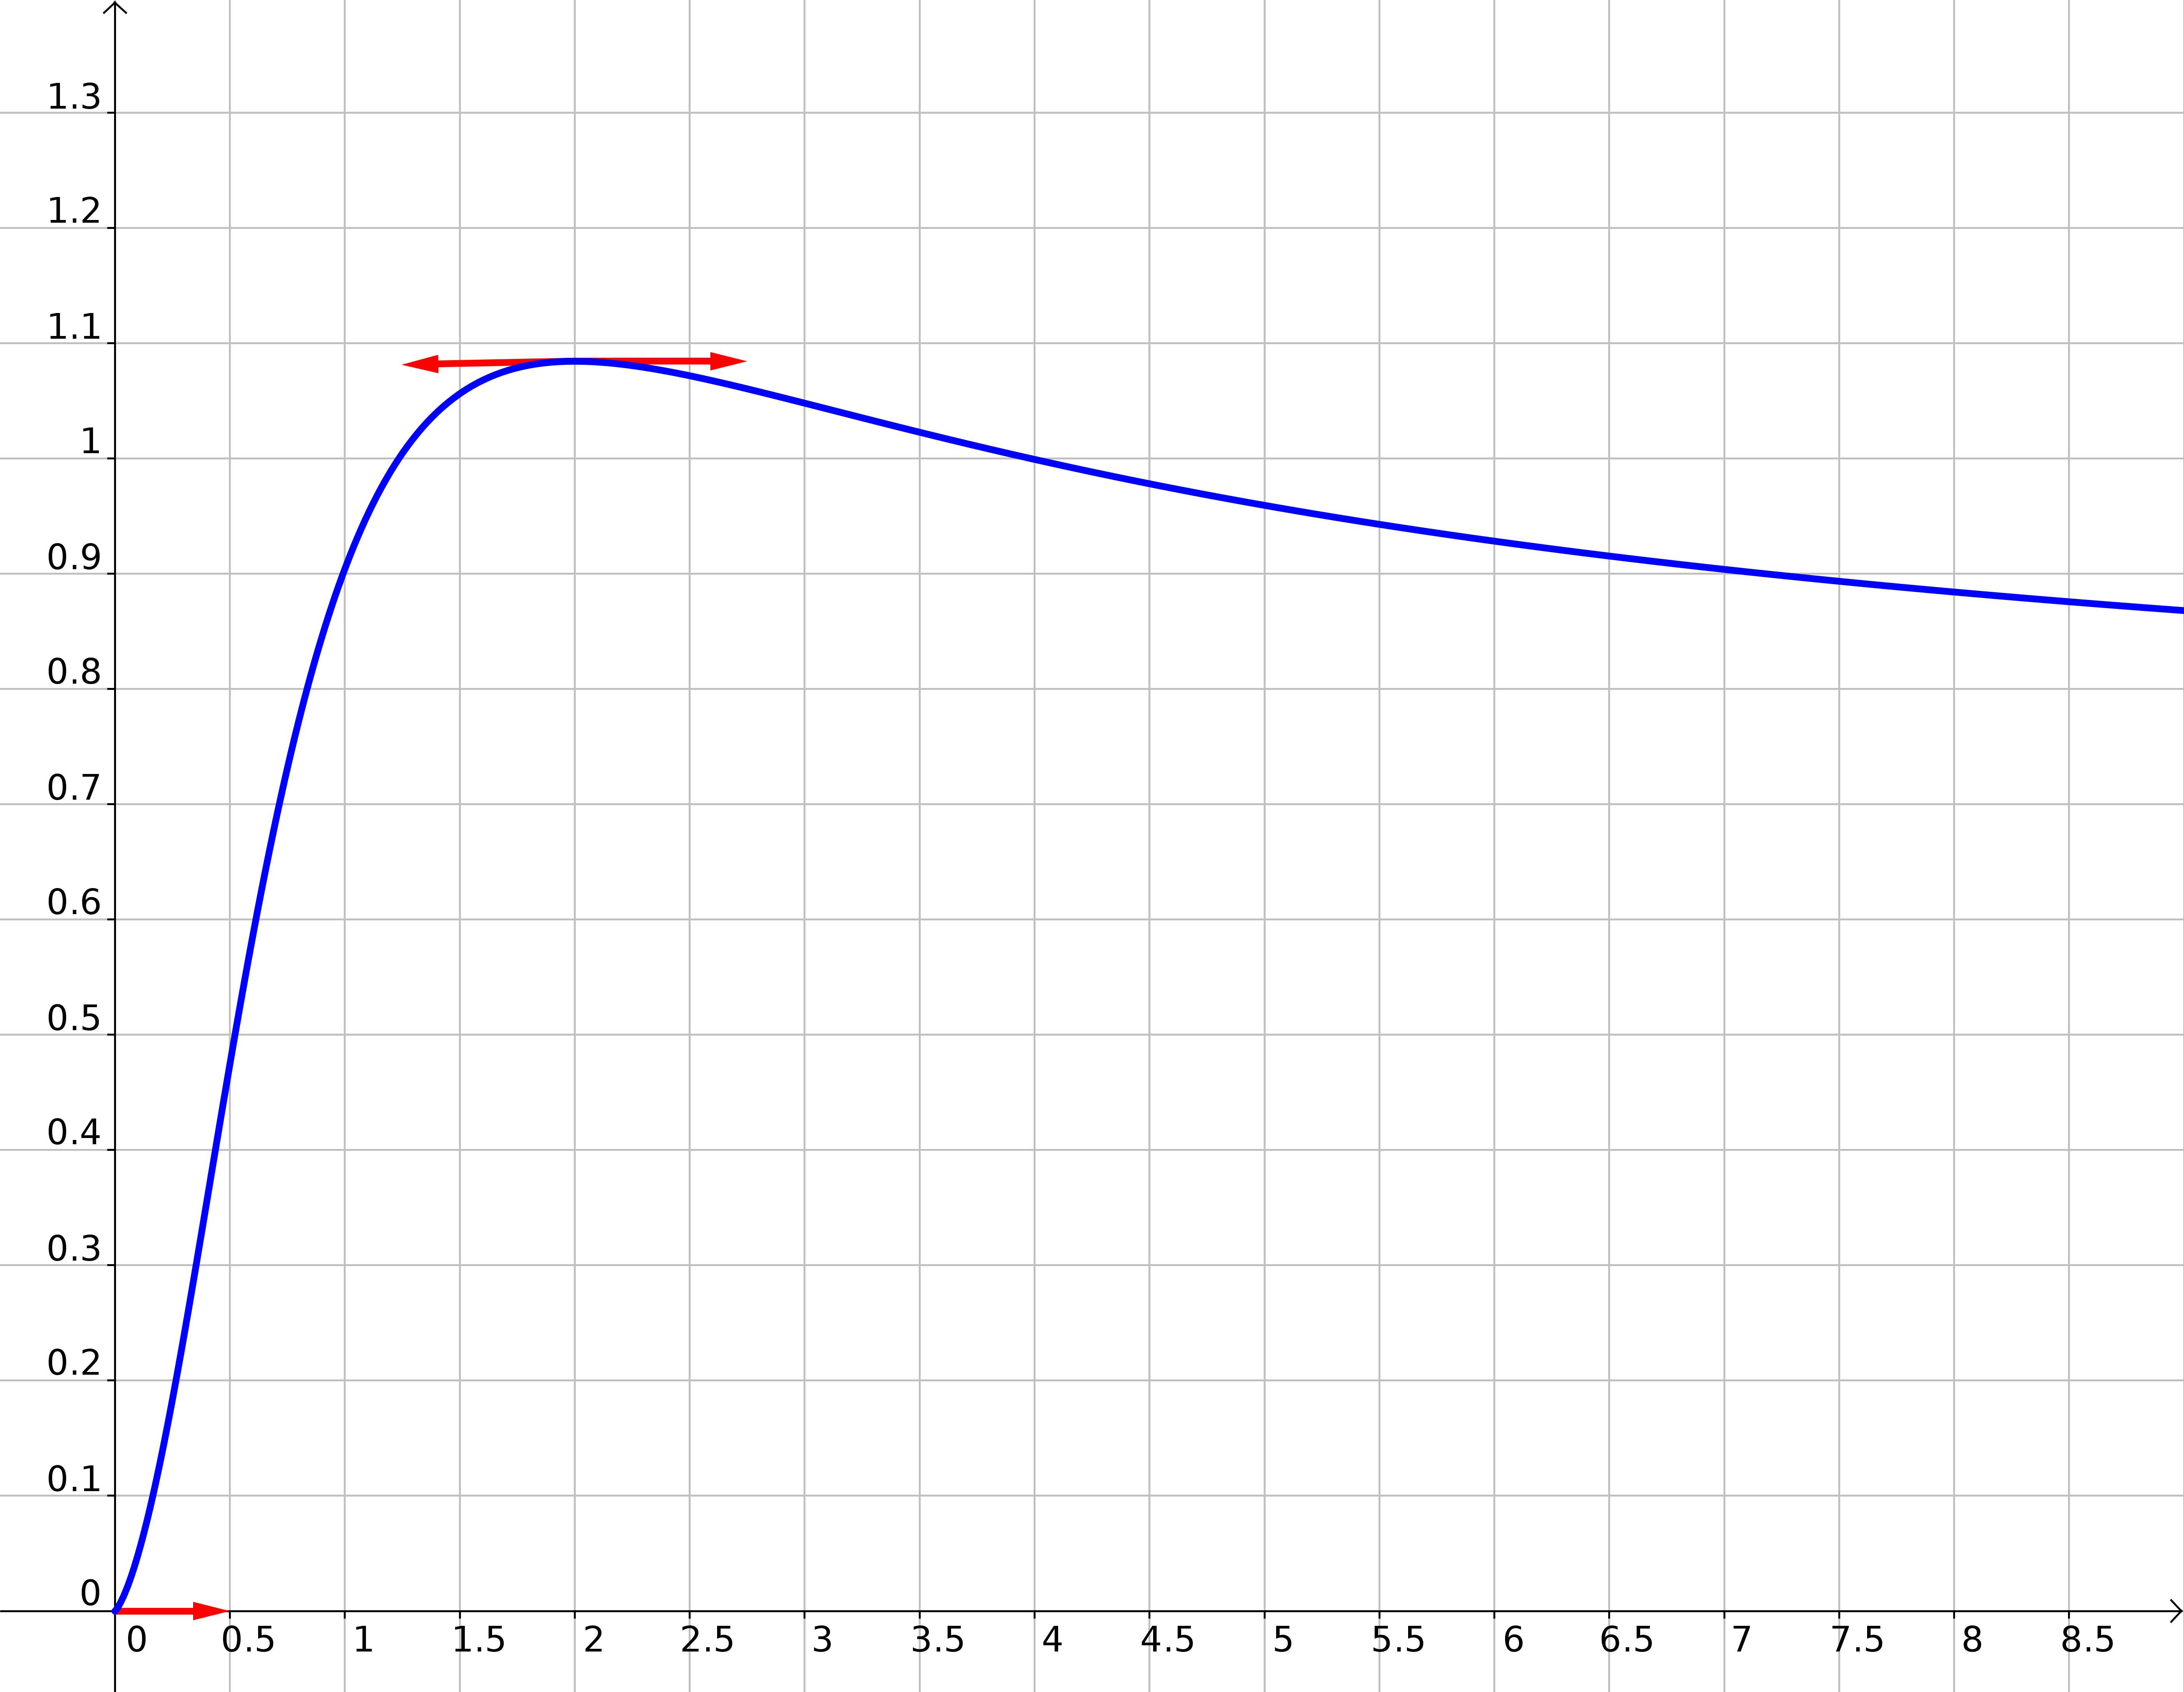
\includegraphics[scale=.25]{Figures/EML_2018/geogebra_EML_2018.png}
      
    \end{center}
    
    \begin{remark}
      Sur le graphe précédent, la tangente à l'origine ne semble pas
      être correcte.\\
      En effet, comme son étymologie (le verbe latin \og tangere
      \fg{}) l'indique, une tangente doit {\bf toucher} la courbe, ce
      qui ne paraît pas être le cas ici.\\
      Cela est simplement dû à l'échelle de la figure. Si on zoome sur
      l'origine du repère, on obtient le graphe suivant :
      \begin{center}
        
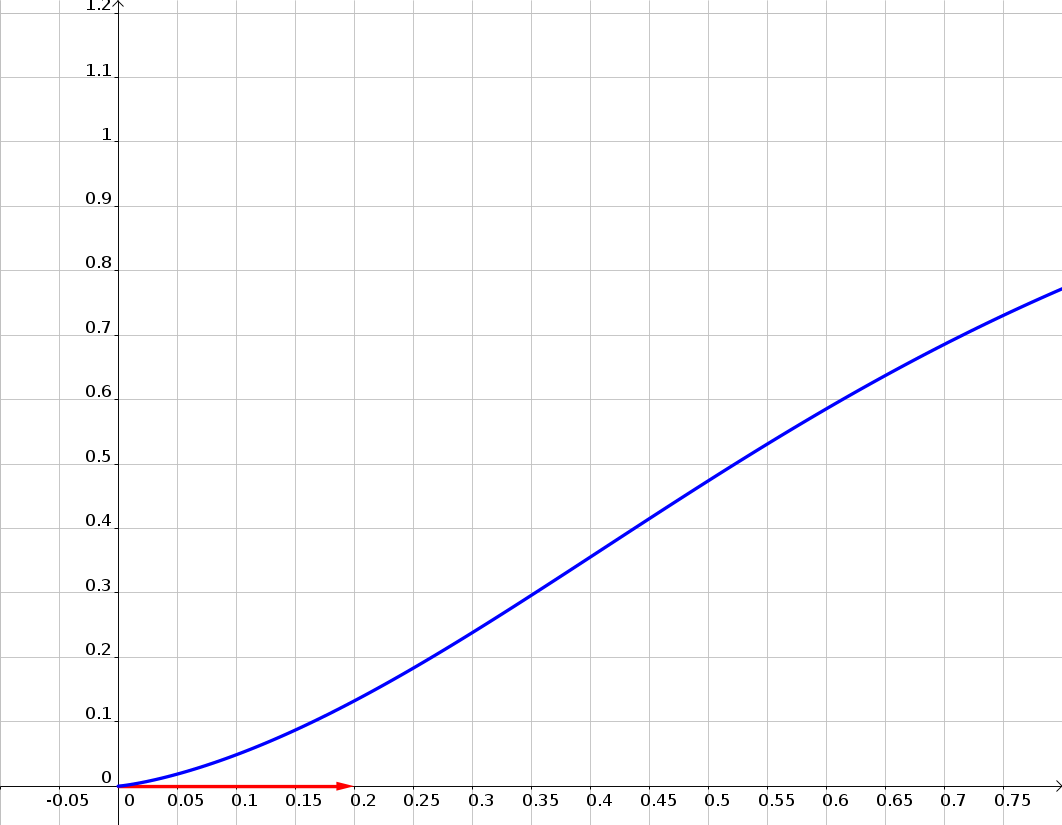
\includegraphics[scale=1]{Figures/EML_2018/geogebra_EML_2018_zoom.png}
      \end{center}
      Sur une copie, il faut bien évidemment accentuer les tangentes 
      à la courbe.
    \end{remark}~\\[-1.4cm]
  \end{proof}
\end{noliste}


\newpage


\subsection*{Partie IV : Étude d'une fonction de deux variables}

\noindent
On considère la fonction $H$ de classe $\Cont{2}$ sur l'ouvert $U = \
]0,+\infty[^2$ définie par :
\[
  \forall (x,y) \in \ ]0,+\infty[^2, \ H(x,y) = \dfrac{x^2}{2} -xy-2x 
  + \ee^y
\]

\begin{remark}
  On peut remarquer que cette fonction $H$ est en fait définie sur 
  $\R^2$. Cela sera d'ailleurs utile plus tard dans l'énoncé. \\
  Elle est même de classe $\Cont{2}$ sur $\R^2$.
  Démontrons le.~\\[-.4cm]
  \begin{noliste}{$\sbullet$}
    \item La fonction $(x,y) \mapsto \dfrac{x^2}{2} -xy -2x$ est de 
    classe $\Cont{2}$ sur $\R^2$ en tant que fonction polynomiale.
    \item La fonction $(x,y) \mapsto \ee^y$ est de classe $\Cont{2}$
    sur $\R^2$ car elle est la composée $h_2 \circ h_1$ où :
    \begin{noliste}{$\stimes$}
      \item $h_1 : (x,y) \mapsto y$ est :
      \begin{noliste}{-}
	\item de classe $\Cont{2}$ sur $\R^2$ en tant que fonction 
	polynomiale,
	\item telle que $h_1(\R^2) \subset \R$.
      \end{noliste}
      \item $h_2: u \mapsto \ee^u$ est de classe $\Cont{2}$ sur $\R$.
    \end{noliste}
    \item La fonction $H$ est donc de classe $\Cont{2}$ sur $\R^2$
    en tant que somme de fonctions de classe $\Cont{2}$ sur $\R^2$.
  \end{noliste}
\end{remark}

\begin{noliste}{1.}
  \setlength{\itemsep}{4mm}
  \setcounter{enumi}{12}
  \item 
  \begin{noliste}{a)}
    \setlength{\itemsep}{2mm}
    \item Calculer les dérivées partielles d'ordre $1$ de $H$ en tout 
    $(x,y)$ de $U$.
    
    \begin{proof}~
      \begin{noliste}{$\sbullet$}
	\item La fonction $H$ est de classe $\Cont{2}$, donc de classe 
	$\Cont{1}$ sur $U$.\\
	Elle admet donc des dérivées partielles d'ordre $1$ sur $U$.
	
	\item Soit $(x,y) \in U$.
	\[
	  \dfn{H}{1}(x,y) \ = \ \dfrac{\bcancel{2} \, x}{\bcancel{2}} -y
	  -2 \ = \ x-y-2
	\]
	\[
	  \dfn{H}{2}(x,y) \ = \ -x + \ee^y
	\]
	\conc{$\forall (x,y) \in U$, $\dfn{H}{1}(x,y) = x-y-2$, 
	\quad $\dfn{H}{2}(x,y) = \ee^y -x$}
      \end{noliste}
      
      \begin{remark}
        On trouve bien sûr les mêmes dérivées premières sur $\R^2$.
      \end{remark}~\\[-1.4cm]
    \end{proof}
    
    
    \newpage
    
    
    \item Montrer que la fonction $H$ admet exactement deux points 
    critiques : $(a, \ln(a))$ et $(b,\ln(b))$, où les réels $a$ et $b$
    sont ceux introduits dans la question \itbf{2.}
    
    \begin{proof}~\\
      Soit $(x,y) \in U$.\\
      Le couple $(x,y)$ est un point critique de $H$ si et seulement 
      si :
      \[
       \begin{array}{rcl@{\qquad}>{\it}R{3cm}}
        \nabla(H)(x,y) = 0_{\M{2,1}} & \Leftrightarrow &
        \left\{
        \begin{array}{rcl}
          \dfn{H}{1}(x,y) & = &  0\\[.1cm]
          \dfn{H}{2}(x,y) & = &  0
        \end{array}
        \right.
        \\[.6cm]
        & \Leftrightarrow & 
        \left\{
        \begin{array}{l}
          x-y-2=0\\[.1cm]
          \ee^y-x=0
        \end{array}
        \right.
        \ \Leftrightarrow \ 
        \left\{
        \begin{array}{l}
          y = x-2\\[.1cm]
          \ee^y=x
        \end{array}
        \right.
        \\[.6cm]
        & \Leftrightarrow &
        \left\{
        \begin{array}{l}
          y = x-2\\[.1cm]
          \ee^{x-2} = x
        \end{array}
        \right.
        \ \Leftrightarrow \ 
        \left\{
        \begin{array}{l}
          y = x-2\\[.1cm]
          x-2 = \ln(x)
        \end{array}
        \right.
        & (car $x>0$)
        \nl
        \nl[-.2cm]
        & \Leftrightarrow &
        \left\{
        \begin{array}{l}
          y = x-2\\[.1cm]
          x- \ln(x) =2
        \end{array}
        \right.
        \ \Leftrightarrow \
        \left\{
        \begin{array}{l}
          y = x-2\\[.1cm]
          f(x) = 2
        \end{array}
        \right.
       \end{array}
      \]
      Or, d'après la question \itbf{2.}, l'équation $f(x)=2$ admet 
      exactement deux solutions sur $]0,+\infty[$ : les réels
      $a$ et $b$.\\
      On obtient donc :
      \[
       \begin{array}{rcl}
        \nabla(H)(x,y)=0_{\M{2,1}} & \Leftrightarrow &
        \left\{
        \begin{array}{l}
          y = x-2\\
          x = a
        \end{array}
        \right.
        \quad \OU \quad 
        \left\{
        \begin{array}{l}
          y = x-2\\
          x = b
        \end{array}
        \right.
        \\[.6cm]
        & \Leftrightarrow &
        \left\{
        \begin{array}{l}
          y = a-2\\
          x = a
        \end{array}
        \right.
        \quad \OU \quad 
        \left\{
        \begin{array}{l}
          y = b-2\\
          x = b
        \end{array}
        \right.
       \end{array}
      \]
      Or, comme $a$ et $b$ sont solutions de l'équation $f(x)=2$, on a :
      \[
        f(b)=2 \ \Leftrightarrow \ b-\ln(b)=2 \ \Leftrightarrow \
        \ln(b)=b-2
      \]
      De même : $\ln(a)=a-2$. D'où :
      \[
       \begin{array}{rcl}
        \text{$(x,y)$ est un point critique de $H$} & \Leftrightarrow &
        \left\{
        \begin{array}{l}
          y = \ln(a)\\
          x = a
        \end{array}
        \right.
        \quad \OU \quad 
        \left\{
        \begin{array}{l}
          y = \ln(b)\\
          x = b
        \end{array}
        \right.
        \\[.6cm]
        & \Leftrightarrow & 
        (x,y)=(a,\ln(a)) \quad \OU \quad (x,y)=(b,\ln(b))
       \end{array}
      \]
      Or, comme $a \in \ ]0,1[$, alors $\ln(a) <0$. Donc 
      $(a, \ln(a)) \notin U$.\\
      On en déduit que le couple $(a,\ln(a))$ n'est pas un point 
      critique de $H$ sur $U$.
      
      \conc{Ainsi, la fonction $H$ admet un unique point 
      critique \underline{sur $U$} : $(b,\ln(b))$.}
      
      
      \newpage
      
      
      \begin{remark}
       \begin{noliste}{$\sbullet$}
        \item La réponse à cette question semble contredire l'énoncé.\\
        En fait, le couple $(a,\ln(a))$ est bien un point critique de 
        $H$. Seulement, c'est un point critique de $H$ \underline{sur 
        $\R^2$} et non \underline{sur $U$}.\\[.1cm]
        Montrer que $(a,\ln(a))$ est bien un point critique de $H$ sur 
        $\R^2$ demande peu d'adaptations dans la preuve précédente.\\
        Le seul point problématique est la 
        composition par la fonction $\ln$ dans la première série 
        d'équivalences :
        \[
          \left\{
          \begin{array}{l}
            y = x-2\\
            \ee^{x-2} = x
          \end{array}
          \right.
          \ \Leftrightarrow \
          \left\{
          \begin{array}{l}
            y = x-2\\[.1cm]
            x-2 = \ln(x)
          \end{array}
          \right.
        \]
        En effet, il faut démontrer auparavant que $x>0$ (a priori :
        $x\in \R$).\\
        Cependant, d'après le système $\left\{
        \begin{array}{l}
          y = x-2\\[.1cm]
          \ee^y = x
        \end{array}
        \right.$, on en déduit en particulier que $x>0$, et on peut donc
        continuer la preuve comme précédemment.
        
        \item Dans la suite, lorsque l'on étudiera le point critique 
        $(a,\ln(a))$, on se placera donc sur $\R^2$ et non sur $U$.
       \end{noliste}
      \end{remark}~\\[-1.4cm]
    \end{proof}
  \end{noliste}
  
  
  \item 
  \begin{noliste}{a)}
    \setlength{\itemsep}{2mm}
    \item Écrire la matrice hessienne, notée $M_a$, de $H$ au point
    $(a,\ln(a))$.
    
    \begin{proof}~
      \begin{noliste}{$\sbullet$}
	\item La fonction $H$ est de classe $\Cont{2}$ sur $\R^2$, elle 
	admet donc des dérivées partielles d'ordre $2$ sur $\R^2$.
	
	\item Soit $(x,y) \in \R^2$.
	\[
	  \nabla^2(H)(x,y) \ = \
	  \begin{smatrix}
	    \ddfn{H}{1,1}(x,y) & \ddfn{H}{1,2}(x,y)
	    \\[.2cm]
	    \ddfn{H}{2,1}(x,y) & \ddfn{H}{2,2}(x,y)
	  \end{smatrix}
	  \ = \
	  \begin{smatrix}
	    1 & -1\\[.2cm]
	    -1 & \ee^y
	  \end{smatrix}
	\]
	\conc{Donc : $M_a = \nabla^2(H)(a,\ln(a)) =
	\begin{smatrix}
	  1 & -1\\
	  -1 & \ee^{\ln(a)}
	\end{smatrix}
	=
	\begin{smatrix}
	  1 & -1\\
	  -1 & a
	\end{smatrix}
	$}
      \end{noliste}
      
      \begin{remark}
	  On rappelle que $(a,\ln(a)) \notin U$.\\
	  Il est donc indispensable de déterminer $\nabla^2(H)$ sur 
	  $\R^2$ et non sur $U$.
	\end{remark}~\\[-1.4cm]
    \end{proof}

    
    \item Montrer que $M_a$ admet deux valeurs propres distinctes, 
    notées $\lambda_1$ et $\lambda_2$, vérifiant 
    \[
      \left\{
      \begin{array}{ccc}
        \lambda_1 + \lambda_2 & = & a+1\\
        \lambda_1 \, \lambda_2 & = & a-1
      \end{array}
      \right.
    \]
    
    \begin{proof}~
      \begin{noliste}{$\sbullet$}
	\item La matrice $M_a$ est une matrice réelle symétrique. Donc 
	elle est diagonalisable.\\
	On note $\lambda_1$ et $\lambda_2$ ses valeurs propres 
	(éventuellement égales).
	
	\item Soit $\lambda \in \R$.
	\[
	 \begin{array}{rcl}
	  \det(M_a - \lambda \cdot I_2) & = &  \det
	  \begin{smatrix}
	    1-\lambda & -1\\
	    -1 & a-\lambda
	  \end{smatrix}
	  \ = \ (1-\lambda)(a-\lambda) -1
	  \\[.6cm]
	  & = &  \lambda^2 - (a+1)\lambda + (a-1)
	 \end{array}
	\]
	
	
	\newpage
	
	
	On en déduit que la matrice $M_a - \lambda \cdot I_2$ n'est 
	pas inversible si et seulement si :
	\[
	  \lambda^2 - (a+1)\lambda + (a-1) = 0 \quad (*)
	\]
	
	\item Or $\lambda_1$ et $\lambda_2$ sont les valeurs propres
	de $M_a$, donc :
	\[
	  \text{$(M_a-\lambda \cdot I_2)$ n'est pas inversible} \ 
	  \Leftrightarrow \
	  \lambda \in \{\lambda_1, \lambda_2 \}
	\]
	Ainsi les réels $\lambda_1$ et $\lambda_2$ sont les racines
	de l'équation $(*)$. D'où :
	\[
	  \lambda^2 - (a+1)\lambda + (a-1) \ = \ (\lambda - 
	  \lambda_1)(\lambda - \lambda_2) \ = \
	  \lambda^2 - (\lambda_1 + \lambda_2) \lambda + \lambda_1 \,
	  \lambda_2
	\]
	\conc{Par identification des coefficients de ces polynômes de 
	degré $2$ en $\lambda$, \\[.1cm]
	on obtient le système suivant :
	$
	  \left\{
	  \begin{array}{l}
	    \lambda_1 + \lambda_2 = a+1\\[.1cm]
	    \lambda_1 \, \lambda_2 = a-1
	  \end{array}
	  \right.
	$}
	
	\item Montrons maintenant que $\lambda_1$ et $\lambda_2$ sont 
	distincts.\\
	Raisonnons par l'absurde. Supposons alors que $\lambda_1 =
	\lambda_2$.\\
	D'après le système précédent, on obtient en particulier :
	\[
	  \lambda_1^2 \ = \ \lambda_1 \, \lambda_2 \ = \ a-1
	\]
	Or, d'après la question \itbf{2.}, on a : $a<1$. Donc $a-1<0$.\\
	On en déduit : $\lambda_1^2 <0$, ce qui est absurde.
	\conc{Ainsi, $\lambda_1$ et $\lambda_2$ sont 
	distincts.}~\\[-1.2cm]
      \end{noliste}
    \end{proof}
    
    
    \item La fonction $H$ présente-t-elle un extremum local au point
    $(a,\ln(a))$ ?
    
    \begin{proof}~\\
      On a montré dans la question précédente : $a-1<0$. On en déduit : 
      $\lambda_1 \, \lambda_2 <0$.\\
      Les valeurs propres de $M_a$ sont donc de signes opposés.
      \conc{Ainsi, la fonction $H$ n'admet pas d'extremum local 
      au point $(a,\ln(a))$.}
      
      \begin{remark}
        Le point $(a,\ln(a))$ est un point selle pour la fonction $H$.
      \end{remark}~\\[-1.4cm]
    \end{proof}
  \end{noliste}
  
  
  \item La fonction $H$ présente-t-elle un extremum local au point 
  $(b,\ln(b))$ ?
  
  \begin{proof}~\\
    On reprend la démarche des questions précédentes.
    \begin{noliste}{$\sbullet$}
      \item On note $M_b$ la matrice hessienne de $H$ au point 
      $(b,\ln(b))$. Alors :
      \[
        M_b \ = \
        \begin{smatrix}
          1 & -1\\
          -1 & \ee^{\ln(b)}
        \end{smatrix}
        \ = \
        \begin{smatrix}
          1 & -1\\
          -1 & b
        \end{smatrix}
      \]
      
      \item La matrice $M_b$ est une matrice réelle symétrique. Donc 
      elle est diagonalisable.\\
      On note $\mu_1$ et $\mu_2$ ses valeurs propres éventuellement 
      égales).
      
      \item Soit $\lambda \in \R$.
      \[
        \det(M_b - \lambda \cdot I_2) \ = \ \lambda^2 - (b+1) \lambda 
        + (b-1)
      \]
      On en déduit que la matrice $M_b - \lambda \cdot I_2$ n'est pas 
      inversible si et seulement si :
      \[
        \lambda^2 - (b+1) \lambda + (b-1) = 0 \quad (\star)
      \]
      
      
      \newpage
      
      
      \item Or $\mu_1$ et $\mu_2$ sont les valeurs propres de $M_b$, 
      donc $\mu_1$ et $\mu_2$ sont les racines de l'équation $(\star)$.
      D'où : 
      \[
        \lambda^2 - (b+1) \lambda + (b-1) \ = \ (\lambda- \mu_1)
        (\lambda - \mu_2) \ = \ \lambda^2 - (\mu_1 + \mu_2) \lambda
        + \mu_1 \, \mu_2
      \]
      \conc{Par identification : $\left\{
      \begin{array}{l}
        \mu_1 + \mu_2 \ = \ b+1\\
        \mu_1 \, \mu_2 \ = \ b-1
      \end{array}
      \right.$.}
      
      \item D'après la question \itbf{3.} : $b \geq 2$. Donc : $b-1 
      > 0$ et $b+1 > 0$.\\
      On obtient alors :
      \begin{noliste}{$\stimes$}
	\item $\mu_1 \, \mu_2 > 0$.\\
	Donc $\mu_1$ et $\mu_2$ sont non nuls et de même signe.
	\item $\mu_1 + \mu_2 >0$.\\
	Or $\mu_1$ et $\mu_2$ ont même signe. Donc : $\mu_1 >0$ et 
	$\mu_2 >0$.
      \end{noliste}
      \conc{On en déduit que la fonction $H$ admet un minimum local en
      $(b,\ln(b))$.}~\\[-1.4cm]
    \end{noliste}
  \end{proof}
\end{noliste}




\section*{Exercice 3}

\noindent
On dispose d'une pièce de monnaie amenant Pile avec la probabilité 
$\dfrac{2}{3}$ et Face avec la probabilité $\dfrac{1}{3}$.

\subsection*{Partie I : Étude d'une première variable aléatoire}

\noindent
On effectue une succession de lancers avec cette pièce et on définit la 
variable aléatoire $X$ prenant la valeur du nombre de Face obtenus 
avant l'obtention du deuxième Pile.

\begin{noliste}{1.}
  \setlength{\itemsep}{4mm}
  \item 
  \begin{noliste}{a)}
    \setlength{\itemsep}{2mm}
    \item Décrire les événements $\Ev{X=0}$, $\Ev{X=1}$, $\Ev{X=2}$
    puis calculer leurs probabilités.
    
    \begin{proof}~\\
      Pour tout $k \in \N^*$, on définit les événements suivants :
      \[
        \begin{array}{rcR{6cm}}
          P_k & : & \og obtenir Pile au $\eme{k}$ lancer \fg{}
          \nl
          \nl[-.2cm]
          F_k & : & \og obtenir Face au $\eme{k}$ lancer \fg{}
        \end{array}
      \]
      \begin{noliste}{$\sbullet$}
	\item L'événement $\Ev{X=0}$ est réalisé si et seulement si on
	n'a obtenu aucun Face avant l'obtention du $\eme{2}$ Pile.\\
	On a donc obtenu successivement deux Pile.
	\conc{Ainsi : $\Ev{X=0} = P_1 \cap P_2$.}
	Les lancers de pièce sont indépendants, donc :
	\[
	  \Prob(\Ev{X=0}) \ = \ \Prob(P_1 \cap P_2) \ = \ 
	  \Prob(P_1) \times \Prob(P_2) \ = \ \dfrac{2}{3} \times 
	  \dfrac{2}{3} \ = \ \dfrac{4}{9}
	\]
	\conc{$\Prob(\Ev{X=0}) = \dfrac{4}{9}$}
	
	\begin{remark}
	  L'énoncé ne précise pas explicitement que les lancers sont
	  indépendants. Cette hypothèse est cependant 
	  raisonnable puisque l'expérience de lancer est répétée dans
	  des conditions identiques.
	\end{remark}
	
	
	\newpage

	
	\item L'événement $\Ev{X=1}$ est réalisé si et seulement si on 
	a obtenu un unique Face avant l'apparition du $\eme{2}$ Pile.\\
	Deux cas se présentent alors :
	\begin{noliste}{$\stimes$}
	  \item soit on a obtenu ce Face avant deux Pile successifs,
	  \item soit on a obtenu ce Face entre les deux premiers Pile.
	\end{noliste}
	\conc{Ainsi : $\Ev{X=1} \ = \ (F_1 \cap P_2 \cap P_3) \, \cup
	\, (P_1 \cap F_2 \cap P_3)$.}
	On obtient alors :
	\[
	  \begin{array}{rcl@{\qquad}>{\it}R{5cm}}
	    \Prob(\Ev{X=1}) & = &  \Prob(F_1 \cap P_2 \cap P_3) \ + \ 
	    \Prob(P_1 \cap F_2 \cap P_3)
	    & (par incompatibilité de $F_1 \cap P_2 \cap P_3$ et 
	    $P_1 \cap F_2 \cap P_3$)
	    \nl
	    \nl[-.2cm]
	    & = &  \Prob(F_1) \, \Prob(P_2) \, \Prob(P_3) \ + \ \Prob(P_1) 
	    \, \Prob(F_2) \, \Prob(P_3)
	    & (par indépendance des lancers)
	    \nl
	    \nl[-.2cm]
	    & = &  \dfrac{1}{3} \times \dfrac{2}{3} \times \dfrac{2}{3}
	    \ + \ \dfrac{2}{3} \times \dfrac{1}{3} \times \dfrac{2}{3}
	    \\[.4cm]
	    & = &  2 \ \dfrac{4}{3^3}
	  \end{array}
	\]
	\conc{$\Prob(\Ev{X=1}) = 2 \ \dfrac{4}{3^3}$}
	
	
	\item On raisonne de la même manière pour l'événement 
	$\Ev{X=2}$.
	\conc{$\Ev{X=2} \ = \ (F_1 \cap F_2 \cap P_3 \cap P_4) \, \cup
	\, (F_1 \cap P_2 \cap F_3 \cap P_4) \, \cup \, (P_1 \cap F_2 
	\cap F_3 \cap P_4)$}
	On obtient alors :
	\[
	  \begin{array}{cl@{\qquad}>{\it}R{4cm}}
	    & \Prob(\Ev{X=2})
	    \\[.2cm]
	    =& \Prob(F_1 \cap F_2 \cap P_3 \cap P_4)
	    + \Prob(F_1 \cap P_2 \cap F_3 \cap P_4) +
	    \Prob(P_1 \cap F_2 \cap F_3 \cap P_4)
	    & (par incompatibilité)
	    \nl
	    \nl[-.2cm]
% 	    & = &  \Prob(F_1) \, \Prob(F_2) \, \Prob(P_3) \, \Prob(P_4)
% 	    \ + \ \Prob(F_1) \, \Prob(P_2) \, \Prob(F_3) \, \Prob(P_4) 
% 	    \ + \ \Prob(P_1) \, \Prob(F_2) \, \Prob(F_3) \, \Prob(P_4)
% 	    & (par indépendance)
% 	    \nl
% 	    \nl[-.2cm]
	    =& \dfrac{1}{3} \times \dfrac{1}{3} \times \dfrac{2}{3}
	    \times \dfrac{2}{3} \ + \ \dfrac{1}{3} \times \dfrac{2}{3}
	    \times \dfrac{1}{3} \times \dfrac{2}{3} \ + \ \dfrac{2}{3}
	    \times \dfrac{1}{3} \times \dfrac{1}{3} \times \dfrac{2}{3}
	    & (par indépendance)
	    \nl
	    \nl[-.2cm]
	    =& 3 \ \dfrac{4}{3^4}
	  \end{array}
	\]
	\conc{$\Prob(\Ev{X=2}) = 3 \ \dfrac{4}{3^4}$}~\\[-1.2cm]
      \end{noliste}
    \end{proof}

    
    \item Montrer : $\forall n \in \N$, $\Prob(\Ev{X=n}) = (n+1) \,
    \dfrac{4}{3^{n+2}}$.
    
    \begin{proof}~\\
      Soit $n\in \N$.
      \begin{noliste}{$\sbullet$}
	\item L'événement $\Ev{X=n}$ est réalisé par les tirages qui 
	contiennent $n$ Face et $2$ Pile.\\
	De tels $(n+2)$-tirages sont entièrement caractérisés par :
	\begin{noliste}{$\stimes$}
	  \item la place du $\nd{2}$ Pile : $1$ choix (le $\eme{(n+2)}$
	  lancer),
	  \item la place du $\er{1}$ Pile : $(n+1)$ choix (du 
	  $\er{1}$ lancer au $\eme{(n+1)}$ lancer).
	\end{noliste}
	Il y a donc $1 \times (n+1) = n+1$ tels $(n+2)$-tirages.
	
	\item Il s'agit alors de savoir qu'elle est la probabilité 
	d'apparition de ces $(n+2)$-tirage.
	\begin{noliste}{-}
	  \item Tout d'abord, tous ces $(n+2)$-tirages ont la même 
	  probabilité d'apparition, car ils comportent tous le 
	  même nombre de Face ($n$) et le même nombre de Pile ($2$).\\
	  Donc en particulier, ils ont la même probabilité
	  d'apparition que le
	  tirage suivant qui réalise l'événement :
	  \[
	    F_1 \cap F_2 \cap \cdots \cap F_n \cap P_{n+1} \cap 
	    P_{n+2}
	  \]
	  
	  
	  \newpage
	  
	  
	  \item Or, comme les lancers sont indépendants :
	  \[
	    \begin{array}{rcl}
	      & &\Prob(F_1 \cap F_2 \cap \cdots \cap F_n \cap P_{n+1} 
	      \cap P_{n+2})
	      \\[.2cm]
	      & = &  \Prob(F_1) \, \Prob(F_2) \, \cdots \, \Prob(F_n) \, 
	      \Prob(P_{n+1}) \, \Prob(P_{n+2})
	      \\[.2cm]
	      & = &  \dfrac{1}{3} \times \dfrac{1}{3} \times \cdots \times 
	      \dfrac{1}{3} \times \dfrac{2}{3} \times \dfrac{2}{3}
	      \\[.4cm]
	      & = &  \left(\dfrac{1}{3}\right)^n \times \left(
	      \dfrac{2}{3}\right)^2 
	      \ = \ \dfrac{1}{3^n} \times \dfrac{4}{3^2}
	      \\[.4cm]
	      & = &  \dfrac{4}{3^{n+2}}
	    \end{array}
	  \]
	\end{noliste}
      \end{noliste}
      \conc{Finalement, on a donc : $\forall n\in \N$, 
      $\Prob(\Ev{X=n}) = (n+1) \ \dfrac{4}{3^{n+2}}$.}
      
      \begin{remark}
        On peut exprimer l'événement $\Ev{X=n}$ à partir des $(P_k)$ 
        et $(F_k)$ :
        \[
          \begin{array}{rccl}
            \Ev{X=n} & = & & (P_1 \, \cap \, F_2 \, \cap \, F_3 \, \cap 
            \, \cdots \, \cap \, F_n \, \cap \, F_{n+1} \, \cap \,
            P_{n+2})
            \\[.2cm]
            & & \cup & (F_1 \, \cap \, P_2 \, \cap \, F_3 \, \cap 
            \, \cdots \, \cap \, F_n \, \cap \, F_{n+1} \, \cap \,
            P_{n+2})
            \\[.2cm]
            & & \cup & (F_1 \, \cap \, F_2 \, \cap \, P_3 \, \cap 
            \, \cdots \, \cap \, F_n \, \cap \, F_{n+1} \, \cap \,
            P_{n+2})
            \\[.2cm]
            & & \vdots &
            \\[.2cm]
            & & \cup & (F_1 \, \cap \, F_2 \, \cap \, F_3 \, \cap 
            \, \cdots \, \cap \, F_n \, \cap \, P_{n+1} \, \cap \,
            P_{n+2})
          \end{array}
        \]
        On voit apparaître le fait que $\Ev{X=n}$ est la réunion de 
	$(n+1)$
        événements incompatibles (on voit bien également que c'est le
        choix de la place du $\er{1}$ Pile qui importe).\\
        Les probabilités de chacun de ces événements sont 
        identiques (égales à $\dfrac{4}{3^{n+2}}$ avec le même 
        calcul que précédemment).\\
        On retrouve bien évidemment le résultat démontré plus haut.
        Seule la présentation de la démonstration diffère.
      \end{remark}~\\[-1.4cm]
    \end{proof}
  \end{noliste}
\end{noliste}



\subsection*{Partie II : Étude d'une expérience en deux étapes}

\noindent
On effectue une succession de lancers avec la pièce précédente jusqu'à 
l'obtention du deuxième Pile ; puis en fonction du nombre $n$ de Face 
obtenus, on place $n+1$ boules dans une urne, les boules étant 
numérotées de $0$ à $n$ et indiscernables au toucher, et enfin on 
pioche au hasard une boule de cette urne.\\[.1cm]
On note toujours $X$ la variable aléatoire prenant la valeur du nombre 
de Face obtenus, et on note $U$ la variable aléatoire prenant la valeur 
du numéro de la boule obtenue. On pose : $V=X-U$.

\begin{noliste}{1.}
  \setlength{\itemsep}{4mm}
  \setcounter{enumi}{1}
  \item 
  \begin{noliste}{a)}
    \setlength{\itemsep}{2mm}
    \item Déterminer l'ensemble des valeurs prises par la variable $U$.
    
    \begin{proof}~\\
      Soit $n\in \N$.\\
      Si l'événement $\Ev{X=n}$ est réalisé, alors l'expérience 
      consiste à piocher parmi les boules numérotées de $0$ à $n$.\\
      Donc la \var $U$ peut prendre toutes les valeurs entières entre 
      $0$ et $n$.\\
      Ceci est valable pour tout $n\in \N$ car $X(\Omega) = \N$.
      \conc{On en déduit : $U(\Omega) = \N$}~\\[-1cm]
    \end{proof}
    
    
    \newpage

    
    \item Déterminer, pour tout $n$ de $\N$, la loi conditionnelle de 
    $U$ sachant $\Ev{X=n}$.
    
    \begin{proof}~\\
      Soit $n\in \N$.\\
      Comme expliqué précédemment, si l'événement $\Ev{X=n}$ est 
      réalisé, alors l'expérience consiste à piocher parmi les boules 
      numérotées de $0$ à $n$. On en déduit :
      \begin{noliste}{$\stimes$}
	\item \dashuline{soit $k \in \llb n+1, \ + \infty \llb$}. 
	\\[.1cm]
	Comme
	il est impossible de piocher une boule de numéro supérieur 
	à $(n+1)$, on a :
	\[
	  \Prob_{\Ev{X=n}}(\Ev{U=k}) = 0
	\]
	
	\item \dashuline{soit $k \in \llb 0,n \rrb$}. \\[.1cm]
	Comme la 
	probabilité de choisir parmi ces 
	$(n+1)$ boules est uniforme, on a :
	\[
	  \Prob_{\Ev{X=n}}(\Ev{U=k}) = \dfrac{1}{n+1}
	\]
      \end{noliste}
      \conc{Finalement : $\forall k \in \llb 0,n \rrb$, 
      $\Prob_{\Ev{X=n}}(\Ev{U=k}) = \dfrac{1}{n+1}$ \quad et 
      \\[.4cm] 
      \quad \quad \quad \quad \quad $\forall k \in \llb n+1, +\infty 
      \llb$, $\Prob_{\Ev{X=n}}(\Ev{U=k})=0$.}
      
      \begin{remark}
        Le caractère uniforme du choix d'une boule est justifiée par :
        \begin{noliste}{$\stimes$}
          \item le fait que les boules sont indiscernables au 
          toucher,
          \item on pioche au hasard dans une urne.
        \end{noliste}
      \end{remark}~\\[-1.4cm]
    \end{proof}

    
    \item En déduire, pour tout $k$ de $\N$ :
    \[
      \Prob(\Ev{U=k}) = \Sum{n=k}{+\infty} \dfrac{1}{n+1} \, 
      \Prob(\Ev{X=n}) \quad \text{puis} \quad \Prob(\Ev{U=k}) = 
      \dfrac{2}{3^{k+1}}
    \]
    
    \begin{proof}~
     \begin{noliste}{$\sbullet$}
      \item Soit $k\in \N$.\\
      La famille $(\Ev{X=n})_{n\in \N}$ est un système complet
      d'événements.\\
      D'après la formule des probabilités totales :
      \[
       \begin{array}{rcl@{\qquad}>{\it}R{6cm}}
        \Prob(\Ev{U=k}) & = &  \Sum{n=0}{+\infty} \Prob(\Ev{X=n} \cap 
        \Ev{U=k})
        \\[.4cm]
        & = &  \Sum{n=0}{+\infty} \Prob(\Ev{X=n}) \, 
        \Prob_{\Ev{X=n}}(\Ev{U=k})
        \\[.4cm]
        & = &  \Sum{n=k}{+\infty} \Prob(\Ev{X=n}) \,
        \Prob_{\Ev{X=n}}(\Ev{U=k})
        & (car : $\forall n < k$, $\Prob_{\Ev{X=n}}(\Ev{U=k})=0$
        d'après la question \itbf{2.b)})
        \nl
        \nl[-.2cm]
        & = &  \Sum{n=k}{+\infty} \Prob(\Ev{X=n}) \, \dfrac{1}{n+1}
        & (d'après la question \itbf{2.b)})
       \end{array}
      \]
      \conc{$\forall k \in \N$, $\Prob(\Ev{U=k}) = \Sum{n=k}{+\infty}
      \dfrac{1}{n+1} \, \Prob(\Ev{X=n})$}
      
      \item D'après la question \itbf{1.b)} : 
      \[
        \forall n \in \N, \ \Prob(\Ev{X=n}) = (n+1) \ \dfrac{4}{3^{n+2}}
      \]
      
      
      \newpage
      
      
      On en déduit :
      \[
       \begin{array}{rcl}
        \Prob(\Ev{U=k}) & = &  \Sum{n=k}{+\infty} \dfrac{1}{\bcancel{n+1}}
        \ \bcancel{(n+1)} \ \dfrac{4}{3^{n+2}}
        \ = \ \dfrac{4}{3^2} \, \Sum{n=k}{+\infty} \dfrac{1}{3^n}
        \\[.6cm]
        & = &  \dfrac{4}{3^2} \, \Sum{n=0}{+\infty} \dfrac{1}{3^{n+k}}
        \ = \ \dfrac{4}{3^{k+2}} \ \Sum{n=0}{+\infty}
        \dfrac{1}{3^n}
        \ = \ \dfrac{4}{3^{k+2}} \ \Sum{n=0}{+\infty} \left(
        \dfrac{1}{3}\right)^n
        \\[.6cm]
        & = &  \dfrac{4}{3^{k+2}} \ \dfrac{1}{1- \frac{1}{3}} \ = \
        \dfrac{4}{3^{k+2}} \ \dfrac{3}{2}
        \\[.6cm]
        & = &  \dfrac{2}{3^{k+1}}
       \end{array}
      \]
      \conc{$\forall k \in \N$, $\Prob(\Ev{U=k}) = 
      \dfrac{2}{3^{k+1}}$}~\\[-1.2cm]
     \end{noliste}
    \end{proof}
    
    \item Montrer que $U$ admet une espérance et une variance et les 
    calculer.
    
    \begin{proof}~
      \begin{noliste}{$\sbullet$}
	\item La \var $U$ admet une espérance si et seulement si la 
	série $\Sum{k\geq 0}{} k \, \Prob(\Ev{U=k})$ converge 
	absolument,
	ce qui équivaut à démontrer sa convergence car la série est 
	à termes positifs.
	
	\item Soit $N\in \N$.
	\[
	  \Sum{k=0}{N} k \, \Prob(\Ev{U=k}) \ = \
	  \Sum{k=1}{N} k \, \Prob(\Ev{U=k}) \ = \
	  \Sum{k=1}{N} k \, \dfrac{2}{3^{k+1}} \ = \
	  \dfrac{2}{3^2} \ \Sum{k=1}{N} k \, \dfrac{1}{3^{k-1}} \ = \
	  \dfrac{2}{3^2} \ \Sum{k=1}{N} k \, \left( \dfrac{1}{3}
	  \right)^{k-1}
	\]
	On reconnaît la somme partielle d'ordre $N$ de la série 
	géométrique dérivée de raison $\dfrac{1}{3}$ (avec $\left\vert 
	\dfrac{1}{3} \right\vert <1$), donc elle converge.
	\conc{Ainsi, la \var $U$ admet une espérance.}
	
	De plus :
	\[
	  \E(U) \ = \
	  \dfrac{2}{3^2} \ \Sum{k=1}{+\infty} k \, \left(\dfrac{1}{3}
	  \right)^{k-1} 
	  \ = \ \dfrac{2}{3^2} \ \dfrac{1}{\big(1-\frac{1}{3}\big)^2}
	  \ = \ \dfrac{2}{3^2} \ \dfrac{1}{\big( \frac{2}{3}\big)^2}
	  \ = \ \dfrac{\bcancel{2}}{\bcancel{3^2}} \ 
	  \dfrac{\bcancel{3^2}}{2^{\bcancel{2}}} \ = \ \dfrac{1}{2}
	\]
	\conc{$\E(U) = \dfrac{1}{2}$}
	
	\item La \var $U$ admet une variance si et seulement si la 
	série $\Sum{k\geq 0}{} k^2 \, \Prob(\Ev{U=k})$ converge 
	absolument,
	ce qui équivaut à démontrer sa convergence car la série est 
	à termes positifs.
	
	\item Soit $N\in \N$.
	\[
	 \begin{array}{rcl}
	  \Sum{k=0}{N} k^2 \, \Prob(\Ev{U=k}) 
	  & = & 
	  \Sum{k=1}{N} \big(k(k-1)+k\big) \, \Prob(\Ev{U=k}) 
	  \\[.4cm]
	  & = &  \Sum{k=1}{N} k(k-1) \, \Prob(\Ev{U=k}) + 
	  \Sum{k=1}{N} k \, \Prob(\Ev{U=k})
	  \\[.4cm]
	  & = &  \Sum{k=2}{N} k(k-1) \, \Prob(\Ev{U=k}) + 
	  \Sum{k=1}{N} k \, \Prob(\Ev{U=k})
	 \end{array}
	\]
	On sait déjà que la série $\Sum{k\geq 1} k \, \Prob(\Ev{U=k})$
	converge et est de somme $\dfrac{1}{2}$, car l'espérance
	$\E(U)$ existe et vaut $\dfrac{1}{2}$.
	
	
	\newpage
	
	
	De plus :
	\[
	  \begin{array}{rcl}
	    \Sum{k=2}{N} k(k-1) \, \Prob(\Ev{U=k})
	    & = &  \Sum{k=2}{N} k(k-1) \ \dfrac{2}{3^{k+1}}
	    \ = \ \dfrac{2}{3^3} \ \Sum{k=2}{N} k(k-1) \, 
	    \dfrac{1}{3^{k-2}}
	    \\[.6cm]
	    & = &  \dfrac{2}{3^3} \ \Sum{k=2}{N} k(k-1) \,
	    \left( \dfrac{1}{3} \right)^{k-2}
	  \end{array}
	\]
	On reconnaît la somme partielle d'ordre $N$ de la série 
	géométrique dérivée seconde de raison $\dfrac{1}{3}$ (avec 
	$\left\vert 
	\dfrac{1}{3} \right\vert <1$), donc elle converge.
	\conc{Ainsi, la \var $U$ admet une variance.}
	
	De plus :
	\[
	 \begin{array}{rcl}
	  \E(U^2) & = & 
	  \dfrac{2}{3^3} \ \Sum{k=1}{+\infty} k(k-1) \, 
	  \left(\dfrac{1}{3} \right)^{k-2} + \dfrac{1}{2} 
	  \ = \ \dfrac{2}{3^3} \ \dfrac{2}{\big(1-\frac{1}{3}\big)^3}
	  + \dfrac{1}{2}
	  \\[.6cm]
	  & = &  \dfrac{2^2}{3^3} \ \dfrac{1}{\big( \frac{2}{3}\big)^3}
	  + \dfrac{1}{2}
	  \ = \ \dfrac{\bcancel{2^2}}{\bcancel{3^3}} \ 
	  \dfrac{\bcancel{3^3}}{2^{\bcancel{3}}} + \dfrac{1}{2}
	  \ = \ \dfrac{1}{2} + \dfrac{1}{2} \ = \ 1
	 \end{array}
	\]
	Enfin, d'après la formule de K{\oe}nig-Huygens :
	\[
	  \V(U) \ = \ \E(U^2) - \big(\E(U)\big)^2
	  \ = \ 1 - \left(\dfrac{1}{2}\right)^2 \ = \
	  1 - \dfrac{1}{4} \ = \ \dfrac{3}{4}
	\]
	\conc{$\V(U) = \dfrac{3}{4}$}
      \end{noliste}
      
      \begin{remark}
        On pouvait résoudre cette question plu rapidement en remarquant
        que la \var $U+1$ suit une loi géométrique de paramètre
        $\dfrac{2}{3}$.
        \begin{noliste}{$\sbullet$}
	  \item En effet :
	  \begin{noliste}{$\stimes$}
	    \item $U(\Omega)=\N$. Donc $(U+1)(\Omega)
	    =\N^*$.
	    \item soit $k\in \N^*$.
	    \[
	      \Prob(\Ev{U+1=k}) \ = \ \Prob(\Ev{U=k-1}) \ = \
	      \dfrac{2}{3^k} \ = \ \dfrac{1}{3^{k-1}} \times 
	      \dfrac{2}{3} \ = \ \left(1-\dfrac{2}{3}\right)^{k-1}
	      \times \dfrac{2}{3}
	    \]
	  \end{noliste}
	  On reconnaît une loi géométrique de paramètre 
	    $\dfrac{2}{3}$.
	    D'où : $U+1 \suit \G{\dfrac{2}{3}}$.
	  
	  \item On en déduit l'espérance et la variance de $U$.
	  \begin{noliste}{$\stimes$}
	    \item Tout d'abord : $\E(U+1) = \dfrac{1}{\frac{2}{3}}
	    =\dfrac{3}{2}$.\\
	    Or, par linéarité de l'espérance : $\E(U+1)=\E(U)+1$.\\
	    D'où : $\E(U) = \dfrac{3}{2}-1 = \dfrac{1}{2}$.
	    
	    \item Ensuite : $V(U+1) = \dfrac{1-\frac{2}{3}}
	    {\big(\frac{2}{3}\big)^2} = \dfrac{\frac{1}{\bcancel{3}}}
	    {\frac{4}{3^{\bcancel{2}}}} = \dfrac{3}{4}$.\\
	    Par propriété de la variance : $V(U+1)=\V(U)$. D'où :
	    $V(U)=\dfrac{3}{4}$.
	  \end{noliste}
        \end{noliste}
      \end{remark}~\\[-1.4cm]
    \end{proof}
  \end{noliste}
  
  
  \newpage
  
  
  \item 
  \begin{noliste}{a)}
    \setlength{\itemsep}{2mm}
    \item Déterminer l'ensemble des valeurs prises par la variable $V$.
    
    \begin{proof}~\\
      Rappelons que $X(\Omega)=\N$. On procède alors par disjonction de 
      cas.\\
      Soit $n\in X(\Omega)= \N$. Supposons que l'événement $\Ev{X=n}$ 
      est réalisé.
      \begin{noliste}{$\sbullet$}
        \item On a donc obtenu $n$ Face avant le $\eme{2}$ Pile.
        \item On doit donc ensuite piocher parmi les boules 
        numérotées de $0$ à $n$. Dans ce cas, la \var $U$ peut 
	prendre toutes les valeurs entières entre $0$ et $n$.
	\item On en déduit que $V=X-U$ peut prendre toutes les 
	valeurs entières entre $n-0$ et $n-n$, c'est-à-dire toutes 
	les valeurs entières entre $0$ et $n$.
      \end{noliste}
      \conc{Ceci étant valable pour tout $n\in X(\Omega) = \N$, on 
      en déduit : $V(\Omega) = \N$.}
      
      \begin{remark}
        On pouvait aussi démontrer que $V(\Omega) = \N$ par double 
        inclusion.
        \begin{noliste}{$\sbullet$}
          \item Par définition des \var $U$ et $X$ : $\forall \omega 
          \in \Omega$, $U(\omega) \leq X(\omega)$.\\
          Donc : $\forall \omega \in \Omega$, $V(\omega) = 
          X(\omega) - U(\omega) \geq 0$.\\
          De plus, les \var $X$ et $U$ prennent des valeurs entières.\\
          On en déduit : $V(\Omega) \subset \N$.
          
          \item Soit $n \in \N$.\\
          L'événement $\Ev{V=n}$ est réalisé par exemple si on 
          obtient d'abord $n$ Face, puis on pioche la boule numérotée 
	  $0$.\\
	  On a ainsi trouvé une réalisation de l'événement $\Ev{V=n}$
	  pour tout $n\in \N$.\\
	  On en déduit : $\N \subset V(\Omega)$.
        \end{noliste}
        Finalement : $V(\Omega) = \N$.
      \end{remark}~\\[-1.4cm]
    \end{proof}
    
    \item Déterminer, pour tout $n$ de $\N$, la loi conditionnelle de 
    $V$ sachant $\Ev{X=n}$.
    
    \begin{proof}~\\
      Soit $n\in \N$. Soit $k\in \N$.\\
      Deux cas se présentent.
      \begin{noliste}{$\sbullet$}
	\item \dashuline{Si $k \in \llb n+1, \, +\infty \llb$}, alors : 
	$\Prob_{\Ev{X=n}}(\Ev{V=k})=0$.\\[.1cm]
	En effet, si l'événement $\Ev{X=n}$ est réalisé, alors la 
	\var $U$ peut prendre des valeurs entre $0$ et $n$, et donc 
	$V$ ne peut prendre une valeur strictement supérieure à $n$.
	
	\item \dashuline{Si $k \in \llb 0,n \rrb$}, alors, d'après
	la question \itbf{2.b)} :
	\[
	 \begin{array}{rcl@{\qquad}>{\it}R{4cm}}
	  \Prob_{\Ev{X=n}}(\Ev{V=k}) & = &  
	  \dfrac{\Prob(\Ev{X=n} \cap \Ev{V=k})}{\Prob(\Ev{X=n})}
	  \ = \ \dfrac{\Prob(\Ev{X=n} \cap \Ev{X-U=k})}
	  {\Prob(\Ev{X=n})}
	  \\[.6cm]
	  & = & 
	  \dfrac{\Prob(\Ev{X=n} \cap \Ev{U=n-k})}{\Prob(\Ev{X=n})}
	  \ = \ 
	  \dfrac{\bcancel{\Prob(\Ev{X=n})} \, 
	  \Prob_{\Ev{X=n}}(\Ev{U=n-k})} {\bcancel{\Prob(\Ev{X=n})}}
	  \\[.6cm]
	  & = &  \Prob_{\Ev{X=n}}(\Ev{U=n-k})
	  \ = \ \dfrac{1}{n+1}
	 \end{array}
	\]
      \end{noliste}
      \conc{Finalement : $\forall k \in \llb 0,n \rrb$, 
      $\Prob_{\Ev{X=n}}(\Ev{V=k}) = \dfrac{1}{n+1}$ \quad et 
      \\[.4cm] 
      \quad \quad \quad \quad \quad $\forall k \in \llb n+1, \, +\infty 
      \llb$, $\Prob_{\Ev{X=n}}(\Ev{V=k})=0$.}~\\[-1cm]
    \end{proof}
    
    
    \newpage

    
    \item En déduire la loi de $V$.
    
    \begin{proof}~\\
      On remarque que, pour tout $n\in \N$, la loi conditionnelle de 
      $V$ par rapport à $\Ev{X=n}$ est la même que la loi 
      conditionnelle de $U$ par rapport à $\Ev{X=n}$.
      \conc{Donc, avec les mêmes calculs qu'à la question \itbf{2.c)},
      on obtient :\\[.1cm] 
      $\forall k \in \N$, $\Prob(\Ev{V=k}) = 
      \dfrac{2}{3^{k+1}}$.}~\\[-1cm]
    \end{proof}
  \end{noliste}
  
  \item Montrer que les variables aléatoires $U$ et $V$ sont 
  indépendantes.
  
  \begin{proof}~\\
    On souhaite montrer dans cette question :
    \[
      \forall (k,j) \in \N^2, \ 
      \Prob(\Ev{U=k} \cap \Ev{V=j}) = \Prob(\Ev{U=k}) \, 
      \Prob(\Ev{V=j})
    \]
    Soit $(k,j) \in \N^2$.
    \begin{noliste}{$\sbullet$}
      \item Tout d'abord :
      \[
        \begin{array}{rcl@{\qquad}>{\it}R{5cm}}
          \Prob(\Ev{U=k} \cap \Ev{V=j}) & = &  
          \Prob(\Ev{U=k} \cap \Ev{X-U=j})
          \\[.2cm]
          & = &  \Prob(\Ev{U=k} \cap \Ev{X=k+j})
          \\[.2cm]
          & = &  \Prob(\Ev{X=k+j}) \, \Prob_{\Ev{X=k+j}}
          (\Ev{U=k})
          \\[.2cm]
          & = &  \bcancel{(k+j+1)} \ \dfrac{4}{3^{k+j+2}} \times 
          \dfrac{1}{\bcancel{k+j+1}}
          & (d'après les questions \itbf{1.b)} et \itbf{2.b)},
          car $k+j \geq k$)
          \nl
          \nl[-.4cm]
          & = &  \dfrac{4}{3^{k+j+2}}
        \end{array}
      \]
      
      \item Ensuite, d'après les questions \itbf{2.c)} et \itbf{3.c)} :
      \[
        \Prob(\Ev{U=k}) \ \Prob(\Ev{V=j}) \ = \ \dfrac{2}{3^{k+1}}
        \times \dfrac{2}{3^{j+1}} \ = \ \dfrac{4}{3^{k+j+2}}
      \]
    \end{noliste}
    On a donc bien : $\forall (k,j) \in \N^2$,
    $\Prob(\Ev{U=k} \cap \Ev{V=j}) \ = \ 
    \Prob(\Ev{U=k}) \ \Prob(\Ev{V=j})$.
    \conc{On en déduit que les \var $U$ et $V$ sont 
    indépendantes.}~\\[-1cm]
  \end{proof}

  
  \item Que vaut $\cov(U,V)$ ? En déduire $\cov(X,U)$ ?
  
  \begin{proof}~
    \begin{noliste}{$\sbullet$}
      \item Les \var $U$ et $V$ sont indépendantes d'après la 
      question précédente.
      
      \conc{On en déduit : $\Cov(U,V)=0$}
      
      \begin{remark}
        Attention ! L'implication suivante n'est pas une équivalence :
        \begin{center}
          $X$ et $Y$ indépendantes \quad $\Rightarrow$ \quad 
          $\Cov(X,Y)=0$
        \end{center}
      \end{remark}
      
      
      \newpage
      
      
      \item On calcule :
      \[
        \begin{array}{rcl@{\qquad}>{\it}R{6cm}}
          \Cov(X,U) & = &  \Cov(U+V,U)
          & (par définition de $V$)
          \nl
          \nl[-.2cm]
          & = &  \Cov(U,U) + \Cov(V,U)
          & (par linéarité à gauche de la covariance)
          \nl
          \nl[-.2cm]
          & = &  \Cov(U,U) + \Cov(U,V)
          & (par symétrie de la covariance)
          \nl
          \nl[-.2cm]
          & = &  \V(U) + 0
          & (par propriété de la covariance et d'après la question 
          précédente)
          \nl
          \nl[-.2cm]
          & = &  \dfrac{3}{4}
          & (d'après la question \itbf{2.d)})
        \end{array}
      \]
      \conc{$\Cov(X,U)=\dfrac{3}{4}$}~\\[-1.6cm]
    \end{noliste}
  \end{proof}
\end{noliste}



\subsection*{Partie III : Étude d'un jeu}

\noindent
Dans cette partie, $p$ désigne un réel de $]0,1[$.\\[.1cm]
Deux individus $A$ et $B$ s'affrontent dans un jeu de Pile ou Face dont 
les règles sont les suivantes :
\begin{noliste}{$\sbullet$}
  \item le joueur $A$ dispose de la pièce amenant Pile avec la 
  probabilité $\dfrac{2}{3}$ et lance cette pièce jusqu'à l'obtention 
  du deuxième Pile ; on note $X$ la \var prenant la 
  valeur du nombre de Face alors obtenus ;
  
  \item le joueur $B$ dispose d'une autre pièce amenant Pile avec la
  probabilité $p$ et lance cette pièce jusqu'à l'obtention d'un Pile ;
  on note $Y$ la \var prenant la valeur du nombre de 
  Face alors obtenus ;
  
  \item le joueur $A$ gagne si son nombre de Face obtenus est inférieur
  ou égal à celui de $B$ ; sinon c'est le joueur $B$ qui gagne.
\end{noliste}
On dit que le jeu est équilibré lorsque les joueurs $A$ et $B$ ont la 
même probabilité de gagner.

\begin{noliste}{1.}
  \setlength{\itemsep}{4mm}
  \setcounter{enumi}{5}
  \item {\bf Simulation informatique}
  \begin{noliste}{a)}
    \setlength{\itemsep}{2mm}
    \item Écrire une fonction \Scilab{} d'en-tête {\tt function x = 
    simule\_X()} qui simule la \var $X$.
    
    \begin{proof}~
      \begin{scilab}~
        & \tcFun{function} \tcVar{x} = simule\_X() \nl %
        & \qquad nbFace = 0 \nl %
        & \qquad nbPile = 0 \nl %
        & \qquad \tcFor{while} nbPile < 2 \nl %
        & \qquad \qquad lancer = grand(1, 1, \ttq{}bin\ttq{}, 2/3) \nl %
        & \qquad \qquad \tcIf{if} lancer == 1 \tcIf{then} \nl %
        & \qquad \qquad \qquad nbPile = nbPile + 1 \nl %
        & \qquad \qquad \tcIf{else} \nl %
        & \qquad \qquad \qquad nbFace = nbFace + 1 \nl %
        & \qquad \qquad \tcIf{end} \nl %
        & \qquad \tcFor{end} \nl %
        & \qquad \tcVar{x} = nbFace \nl %
        & \tcFun{endfunction}
      \end{scilab}
      
      
      %\newpage

      
      Détaillons ce programme.
      \begin{noliste}{$\sbullet$}
	\item On s'intéresse au nombre de Pile et au nombre de Face 
	obtenus dans l'expérience.\\
	On initialise donc ces deux variables.
	\begin{scilabC}{1}
	  & \qquad nbFace = 0 \nl %
	  & \qquad nbPile = 0
	\end{scilabC}
	
	
	\newpage

	
        \item On veut ensuite simuler l'expérience décrite par 
	l'énoncé.\\
        On veut donc simuler des lancers de pièces où la 
        probabilité d'obtenir Pile est $\dfrac{2}{3}$ tant 
        qu'on n'a pas obtenu le $\eme{2}$ Pile.
        On traduit cette condition avec une boucle {\tt while} :
        \begin{scilabC}{3}
          & \qquad \tcFor{while} nbPile < 2
        \end{scilabC}

        
        \item Un lancer de pièce est une épreuve de Bernoulli de succès 
	Pile.\\
	Ainsi on simule un lancer avec une \var, notée $Y$, de 
	loi de Bernoulli de paramètre $\dfrac{2}{3}$.\\
	La \var $Y$ prend la valeur $1$ si et seulement si on obtient
	un Pile, et la valeur $0$ sinon.\\
	On simule la \var $Y$ dans la variable {\tt lancer}.
	\begin{scilabC}{4}
	  & \qquad \qquad lancer = grand(1, 1, \ttq{}bin\ttq{}, 2/3)
	\end{scilabC}
	
	\item À chaque lancer, si la variable {\tt lancer} vaut $1$ 
	(c'est-à-dire si on a obtenu Pile), alors on veut augmenter de 
	$1$ le nombre de Pile.
	Si la variable {\tt lancer} vaut $0$ (c'est-à-dire si on a 
	obtenu Face), alors on veut augmenter de $1$ le nombre de 
	Face.
	\begin{scilabC}{5}
	  & \qquad \qquad \tcIf{if} lancer == 1 \tcIf{then} \nl %
	  & \qquad \qquad \qquad nbPile = nbPile + 1 \nl %
	  & \qquad \qquad \tcIf{else} \nl %
	  & \qquad \qquad \qquad nbFace = nbFace + 1 \nl %
	  & \qquad \qquad \tcIf{end} \nl %
	\end{scilabC}
	
	\item La boucle {\tt while} s'arrête dès que {\tt nbPile} vaut 
	$2$.\\
	La réalisation de $X$ obtenue est alors stockée dans la 
	variable {\tt nbFace}.
	\begin{scilabC}{11}
	  & \qquad \tcVar{x} = nbFace
	\end{scilabC}
      \end{noliste}
      
%       \begin{remark}
%         On décrit ici de manière précise les instructions afin 
% 	d'aider le lecteur un peu moins habile en \Scilab{}.\\
% 	Cependant, l'écriture du script démontre la compréhension 
% 	de toutes les commandes en question et permet à coup sûr 
% 	d'obtenir la totalité des points alloués à cette question.
%       \end{remark}
      
      \begin{remark}
        De manière plus élégante, on aurait pu éviter la 
        structure conditionnelle avec ce script :
        \begin{scilab}~
	  & \tcFun{function} \tcVar{x} = simule\_X() \nl %
	  & \qquad nbFace = 0 \nl %
	  & \qquad nbPile = 0 \nl %
	  & \qquad \tcFor{while} nbPile < 2 \nl %
	  & \qquad \qquad lancer = grand(1, 1, \ttq{}bin\ttq{}, 2/3) \nl 
	  %
	  & \qquad \qquad nbPile = nbPile + lancer \nl %
	  & \qquad \qquad nbFace = nbFace + (1-lancer) \nl %
	  & \qquad \tcFor{end} \nl %
	  & \qquad \tcVar{x} = nbFace \nl %
	  & \tcFun{endfunction}
	\end{scilab}
	En effet, comme précisé précédemment :
	\begin{noliste}{$\stimes$}
	  \item si {\tt lancer} vaut $1$, alors {\tt nbPile} 
	  augmente de $1$,
	  \item si {\tt lancer} vaut $0$, alors {\tt nbPile}
	  n'augmente pas.
	\end{noliste}
	De même :
	\begin{noliste}{$\stimes$}
	  \item si {\tt lancer} vaut $1$, alors {\tt nbFace} 
	  n'augmente pas,
	  \item si {\tt lancer} vaut $0$, alors {\tt nbFace}
	  augmente de $1$.
	\end{noliste}
	On obtient bien :
	\begin{scilabC}{5}
	  & \qquad \qquad nbPile = nbPile + lancer \nl
	  & \qquad \qquad nbFace = nbFace + (1-lancer)
	\end{scilabC}
    \end{remark}
    
    
    \newpage
    
        
      \begin{remark}
        Encore plus élégamment, on aurait pu aussi proposer le 
	script suivant qui n'utilise pas de structure itérative :
        \begin{scilab}~
	  & \tcFun{function} \tcVar{x} = simule\_X() \nl %
	  & \qquad PremierPile = grand(1, 1, \ttq{}geom\ttq{}, 2/3) \nl 
	  %
	  & \qquad DeuxiemePile = grand(1, 1, \ttq{}geom\ttq{}, 2/3) \nl 
	  %
	  & \qquad \tcVar{x} = PremierPile + DeuxiemePile - 2 \nl %
	  & \tcFun{endfunction}
	\end{scilab}
        On utilise ici : 
        \begin{noliste}{$\stimes$}
        \item le fait que lors d'une succession d'une 
        infinité d'épreuves de Bernoulli identiques et indépendantes, 
        la loi de la \var associée au premier Pile est une loi 
        géométrique (ici de paramètre $\dfrac{2}{3}$)
        
        \begin{scilabC}{1}
          & \qquad PremierPile = grand(1, 1, \ttq{}geom\ttq{}, 2/3)
        \end{scilabC}
        
        \item le fait que les lancers sont indépendants. Donc la \var 
	associée au deuxième Pile est indépendante de la \var 
	associée au premier Pile.\\
	Elle suit la même loi géométrique (de paramètre $\dfrac{2}{3}$).
	\begin{scilabC}{1}
          & \qquad DeuxiemePile = grand(1, 1, \ttq{}geom\ttq{}, 2/3)
        \end{scilabC}
        
        \item le fait que le nombre de Face obtenus avant de deuxième 
        Pile correspond au nombre total de lancers jusqu'au 
        deuxième Pile ({\tt PremierPile + DeuxiemePile}) auquel 
        on retranche les deux lancers pour lesquels on a obtenu Pile.\\
        On obtient :
        \begin{scilabC}{3}
          & \qquad \tcVar{x} = PremierPile + DeuxiemePile - 2
        \end{scilabC}
        \end{noliste}
      \end{remark}~\\[-1.4cm]
    \end{proof}

    
    \item On suppose que l'on dispose d'une fonction {\tt simule\_Y}
    qui, prenant en argument un réel $p$ de $]0,1[$, simule la variable
    aléatoire $Y$. Expliquer ce que renvoie la fonction suivante :
    
    \begin{scilab}
      & \tcFun{function} \tcVar{r} = mystere(\tcVar{p}) \nl %
      & \qquad \tcVar{r} = 0 \nl %
      & \qquad N = 10\puis{}4 \nl %
      & \qquad \tcFor{for} k = 1:N \nl %
      & \qquad \qquad x = simule\_X() \nl %
      & \qquad \qquad y = simule\_Y(\tcVar{p}) \nl %
      & \qquad \qquad \tcIf{if} x <= y \tcIf{then} \nl %
      & \qquad \qquad \qquad \tcVar{r} = \tcVar{r} + 1/N \nl %
      & \qquad \qquad \tcIf{end} \nl %
      & \qquad \tcFor{end} \nl %
      & \tcFun{endfunction}
    \end{scilab}
    
    \begin{proof}~
      \begin{noliste}{$\sbullet$}
        \item Cette fonction permet d'obtenir une approximation de 
        la probabilité $\Prob(\Ev{X \leq Y})$ en fonction du 
        paramètre $p$.
        
        
        \newpage
        
        
        \item L'idée naturelle pour obtenir cette approximation est :
        \begin{noliste}{$\stimes$}
	  \item de simuler un grand nombre de fois ($N=10^{4}$ est ce
	  grand nombre) les \var $X$ et $Y$.\\
	  Formellement, on souhaite obtenir un $N$-uplet 
	  $(x_1, \ldots, x_N)$ qui correspond à l'observation d'un 
	  $N$-échantillon $(X_1, \ldots, X_N)$ de la \var $X$, et un 
	  $N$-uplet $(y_1, \ldots, y_N)$ qui correspond à l'observation 
	  d'un $N$-échantillon $(Y_1, \ldots, Y_N)$ de la \var $Y$.
	  
	  \item de compter le nombre de fois où $x_i \leq y_i$, pour 
	  $i \in \llb 1, N\rrb$.
        \end{noliste}
        Cette idée est justifiée par la loi faible des grands nombres 
        (LfGN) qui affirme :
        \[
          \dfrac{\text{nombre de fois où $x_i \leq y_i$}}
          {\text{taille de l'observation}} \ \simeq \ \Prob(\Ev{X 
	  \leq Y})
        \]
        
        \item Dans la fonction, les valeurs $(x_1, \ldots, x_N)$ et 
        $(y_1, \ldots, y_N)$ sont obtenues par des appels successifs 
        (à l'aide d'une boucle {\tt for}) aux fonctions {\tt simule\_X}
        et {\tt simule\_Y} et stockées les unes après les autres dans 
        les variables {\tt x} et {\tt y}.
        \begin{scilabC}{3}
          & \qquad \tcFor{for} k = 1:N \nl %
	  & \qquad \qquad x = simule\_X() \nl %
	  & \qquad \qquad y = simule\_Y(\tcVar{p})
        \end{scilabC}
        
        La variable {\tt r} est alors mise à jour à chaque tour de 
        boucle :
        \begin{scilabC}{6}
          & \qquad \qquad \tcIf{if} x <= y \tcIf{then} \nl %
	  & \qquad \qquad \qquad \tcVar{r} = \tcVar{r} + 1/N \nl %
	  & \qquad \qquad \tcIf{end}
        \end{scilabC}
        Détaillons cette mise à jour :
        \begin{noliste}{$\stimes$}
	  \item \dashuline{si {\tt x $\leq$ y}}, alors on effectue 
	  l'instruction {\tt \tcVar{r} = \tcVar{r} + 1/N}.\\
	  Ainsi, à chaque fois que {\tt x $\leq$ y}, la variable 
	  {\tt r} vaut successivement : $\dfrac{1}{N}$, $\dfrac{2}{N}$,
	  $\ldots$, $\dfrac{j}{N}$, où $j$ est le nombre de fois,
	  parmi les $N$ observations, où {\tt x $\leq$ y}.
	  
	  \item \dashuline{si {\tt x $>$ y}}, alors la variable {\tt r}
	  n'est pas mise à jour.
        \end{noliste}
        Cela signifie que la variable {\tt r} compte le nombre de 
        fois où {\tt x $\leq$ y} et divise ce nombre par {\tt N}.\\
        Une fois cette boucle effectuée, la variable {\tt r} 
        contient donc l'approximation de $\Prob(\Ev{X \leq Y})$ 
	formulée par la LfGN.
      \end{noliste}
      \conc{La fonction {\tt mystere} renvoie une approximation 
      de la probabilité $\Prob(\Ev{X \leq Y})$ \\[.1cm]
      pour différentes 
      valeurs de $p$.}~\\[-1cm]
    \end{proof}

    
    \item On trace, en fonction de $p$, une estimation de la 
    probabilité que $A$ gagne et on obtient le graphe suivant :
   
    \begin{center}
      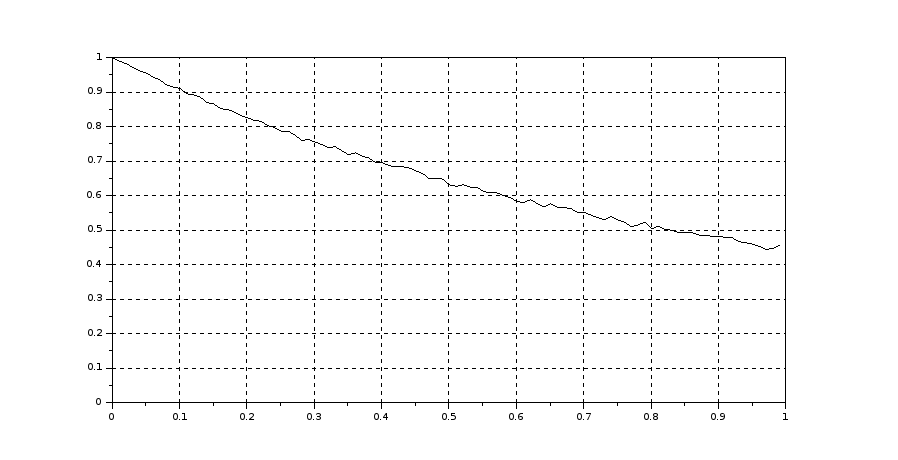
\includegraphics[scale=.4]{Figures/EML_2018/graphe_EML.png}
    \end{center}
    
    À la vue de ce graphe, conjecturer une valeur de $p$ pour laquelle 
    le jeu serait équilibré.
    
    \newpage
    
    \begin{proof}~
     \begin{noliste}{$\sbullet$}
      \item D'après l'énoncé, le jeu est équilibré si les joueurs $A$
      et $B$ ont la même probabilité de gagner, autrement dit si 
      la probabilité que le joueur $A$ gagne vaut $\dfrac{1}{2}$.
      
      \item La probabilité que le joueur $A$ gagne se lit sur l'axe 
      des ordonnées du graphe.\\
      On constate qu'elle vaut $\dfrac{1}{2}$ pour une valeur de $p$
      à peu près égale à $0,82$.
     \end{noliste}
     \conc{On conjecture que la valeur de $p$ pour laquelle le jeu 
     est équilibré est $0,83$.}~\\[-1cm]
    \end{proof}
  \end{noliste}
  
  \item {\bf Étude de la variable aléatoire $Y$}\\[.1cm]
  On note $Z$ la variable aléatoire prenant la valeur du nombre de 
  lancers effectués par le joueur $B$.
  \begin{noliste}{a)}
    \setlength{\itemsep}{2mm}
    \item Reconnaître la loi de $Z$ et préciser son (ses) paramètre(s), 
    son espérance et sa variance.
    
    \begin{proof}~
      \begin{noliste}{$\sbullet$}
	\item Pour le joueur $B$, l'expérience consiste en la 
	succession d'une infinité d'épreuves de Bernoulli 
	identiques et indépendantes de succès Pile, de probabilité $p$.
	
	\item La \var $Z$ est la \var associée au rang d'obtention 
	du premier Pile, donc du premier succès.
      \end{noliste}
      \conc{On en déduit : $Z \suit \G{p}$.\\[.1cm]
      $\E(Z) = \dfrac{1}{p}$ \quad et \quad $\V(Z) = 
      \dfrac{1-p}{p^2}$}~\\[-1cm]
    \end{proof}

    
    \item Exprimer $Y$ à l'aide de $Z$ et en déduire l'existence de 
    l'espérance et de la variance de $Y$ et préciser leurs valeurs.
    
    \begin{proof}~
     \begin{noliste}{$\sbullet$}
      \item Le joueur $B$ arrête de jouer lorsqu'il obtient son premier 
      Pile.\\
      Il a donc obtenu un nombre de Face égal à son nombre de lancers 
      moins $1$ (le dernier lancer pour lequel il a obtenu Pile).
      \conc{$Y=Z-1$}
      
      \conc{La \var $Y$ admet donc une espérance et une variance en 
      tant que \\
      transformée affine d'une \var qui en admet.}
      
      \item Par linéarité de l'espérance :
      \[
        \E(Y) \ = \ \E(Z-1) \ = \ \E(Z)-1 \ = \ \dfrac{1}{p} -1
        \ = \ \dfrac{1-p}{p}
      \]
      \conc{$\E(Y) = \dfrac{1-p}{p}$}
      
      \item Par propriété de la variance :
      \[
        \V(Y) \ = \ \V(Z-1) \ = \ \V(Z) \ = \ \dfrac{1-p}{p^2}
      \]
      \conc{$\V(Y) = \dfrac{1-p}{p^2}$}~\\[-1.2cm]
     \end{noliste}
    \end{proof}
    
    
    \newpage

    
    \item Montrer : $\forall n \in \N, \ \Prob(\Ev{Y \geq n}) = 
    (1-p)^n$.
    
    \begin{proof}~
      \begin{noliste}{$\sbullet$}
	\item On rappelle que $Z \suit \G{p}$. Donc $Z(\Omega) = \N^*$.
	\conc{Comme $Y=Z-1$, on a : $Y(\Omega) = \N$.}
	
	\item Si $n=0$, alors $\Ev{Y \geq 0}=\Omega$ car $Y(\Omega)
	= \N$. Donc :
	\[
	  \Prob(\Ev{Y \geq 0}) \ = \ \Prob(\Omega) \ = \ 1 \ = \
	  (1-p)^0
	\]
	
	\item Soit $n\in \N^*$.
	\[
	  \begin{array}{rcl@{\qquad}>{\it}R{4cm}}
	    \Prob(\Ev{Y\geq n}) & = &  \Prob(\Ev{Z-1 \geq n}) \ = \
	    \Prob(\Ev{Z \geq n+1}) 
	    \\[.2cm]
	    & = &  1 - \Prob(\Ev{Z < n+1})
	    \ = \ 1- \Prob(\Ev{Z \leq n})
	    & (car $Z$ est à valeurs entières)
	  \end{array}
	\]
	Or : $\Ev{Z \leq n} \ = \ \dcup{k=1}{n} \Ev{Z=k}$.\\[.1cm]
	Les événements $\Ev{Z=1}$, $\ldots$, $\Ev{Z=n}$ sont 
	incompatibles. Donc :
	\[
	  \begin{array}{rcl}
	    \Prob(\Ev{Z \leq n}) & = &  \Sum{k=1}{n} \Prob(\Ev{Z=k})
	    \ = \ \Sum{k=1}{n} p \, (1-p)^{k-1}
	    \\[.4cm]
	    & = &  p \ \Sum{k=1}{n} (1-p)^{k-1} \ = \
	    p \ \Sum{k=0}{n-1} (1-p)^k
	    \\[.4cm]
	    & = &  p \ \dfrac{1-(1-p)^n}{\bcancel{1}-(\bcancel{1}-p)} \ = \
	    \bcancel{p} \ \dfrac{1-(1-p)^n}{\bcancel{p}}
	    \\[.6cm]
	    & = &  1-(1-p)^n
	  \end{array}
	\]
	On en déduit :
	\[
	  \Prob(\Ev{Y \geq n}) \ = \ \bcancel{1} - \Big(\bcancel{1}
	  - (1-p)^n \Big) \ = \ (1-p)^n
	\]
      \end{noliste}
      \conc{Finalement : $\forall n \in \N$, $\Prob(\Ev{Y \geq n}) = 
      (1-p)^n$.}
      
      \begin{remark}
	Soit $n\in \N$.\\
        On aurait aussi pu résoudre cette question en exprimant 
        l'événement $\Ev{Y \geq n}$ en fonction des événements :
        \[
          \forall i \in \llb 1,n \rrb, \
          F_i \ = \ \text{\og obtenir Face au $\eme{i}$ lancer}
        \]
        En effet, comme la \var $Y$ est le nombre de Face obtenus 
        avant l'obtention du premier Pile, on a :
        \[
          \Ev{Y \geq n} \ = \ F_1 \cap F_2 \cap \cdots \cap F_n
          \ = \ \dcap{i=1}{n} F_i
        \]
        Comme les lancers sont indépendants, on en déduit :
        \[
          \begin{array}{rcl}
            \Prob(\Ev{ Y \geq n}) & = &  \Prob\left(\dcap{i=1}{n} 
	    F_i\right) \ = \ \Prod{i=1}{n} \Prob(F_i)
	    \\[.4cm]
	    & = &  \Prod{i=1}{n} (1-p) \ = \ (1-p)^n
          \end{array}
        \]
      \end{remark}~\\[-1.4cm]
    \end{proof}
  \end{noliste}
  
  
  \newpage
  
  
  \item 
  \begin{noliste}{a)}
    \setlength{\itemsep}{2mm}
  \item Montrer : $\Prob(\Ev{X \leq Y}) = \Sum{n=0}{+\infty}
    \Prob(\Ev{X=n}) \, \Prob(\Ev{Y \geq n})$.
    
    \begin{proof}~\\
      La famille $(\Ev{X=n})_{n\in \N}$ est un système complet 
      d'événements.\\
      D'après la formule des probabilités totales :
      \[
        \begin{array}{rcl@{\qquad}>{\it}R{4cm}}
          \Prob(\Ev{X \leq Y}) & = &  \Sum{n=0}{+\infty} 
          \Prob(\Ev{X=n} \cap \Ev{X \leq Y})
          \\[.4cm]
          & = &  \Sum{n=0}{+\infty} \Prob(\Ev{X=n} \cap \Ev{n \leq Y})
          \\[.4cm]
          & = &  \Sum{n=0}{+\infty} \Prob(\Ev{X=n}) \ 
          \Prob(\Ev{n \leq Y})
          & (car les \var $X$ et $Y$ sont indépendantes)
        \end{array}
      \]
      Les \var $X$ et $Y$ sont indépendantes, car les lancers du joueur
      $A$ et ceux du joueur $B$ sont indépendants.
      \conc{On a bien : $\Prob(\Ev{X \leq Y}) = 
      \Sum{n=0}{+\infty} \Prob(\Ev{X=n}) \ \Prob(\Ev{Y \geq 
      n})$.}~\\[-1cm]
    \end{proof}
    
  \item Déduire des résultats précédents : $\Prob(\Ev{X \leq Y}) =
    \dfrac{4}{(2+p)^2}$.
    
    \begin{proof}~\\
      D'après les questions \itbf{1.b)} et \itbf{7.b)} et la question 
      précédente :
      \[
        \begin{array}{rcl}
          \Prob(\Ev{X \leq Y}) & = &  \Sum{n=0}{+\infty}
          \Prob(\Ev{X=n}) \ \Prob(\Ev{Y \geq n})
          \ = \ \Sum{n=0}{+\infty} \Big( (n+1) \ \dfrac{4}{3^{n+2}} \
          (1-p)^n\Big)
          \\[.4cm]
          & = &  \dfrac{4}{3^2} \ \Sum{n=0}{+\infty} \Big( (n+1) \ 
          \dfrac{1}{3^n} \ (1-p)^n \Big)
          \ = \ \dfrac{4}{3^2} \ \Sum{n=0}{+\infty} (n+1) \
          \left( \dfrac{1-p}{3}\right)^n
          \\[.4cm]
          & = &  \dfrac{4}{3^2} \ \Sum{n=1}{+\infty} n \ \left(
          \dfrac{1-p}{3}\right)^{n-1} 
        \end{array}
      \]
      On reconnaît la somme d'une série géométrique dérivée de raison 
      $\dfrac{1-p}{3}$ (avec $\left\vert \dfrac{1-p}{3} \right\vert 
      <1$), donc elle converge bien.\\
      On obtient :
      \[
        \Prob(\Ev{X \leq Y}) \ = \ \dfrac{4}{3^2} \ 
        \dfrac{1}{\Big(1- \frac{1-p}{3}\Big)^2}
        \ = \ \dfrac{4}{3^2} \ \dfrac{1}{\Big(\frac{2+p}{3}\Big)^2}
        \ = \ \dfrac{4}{\bcancel{3^2}} \ 
        \dfrac{\bcancel{3^2}}{(2+p)^2} \ = \ 
        \dfrac{4}{(2+p)^2}
      \]
      \conc{$\Prob(\Ev{X \leq Y}) = \dfrac{4}{(2+p)^2}$}~\\[-1cm]
    \end{proof}

    
    \item Déterminer la valeur de $p$ pour lequel le jeu est équilibré.
    
    \begin{proof}~
      \begin{noliste}{$\sbullet$}
	\item D'après l'énoncé, le jeu est équilibré si les joueurs $A$
	et $B$ ont la même probabilité de gagner.
	
	\item Or le joueur $A$ gagne si son nombre de Face obtenus est 
	inférieur ou égal à celui du joueur $B$, c'est-à-dire si 
	l'événement $\Ev{X \leq Y}$ est réalisé.\\
	Sinon le joueur $A$ perd.
	
	
	\newpage
	
	
	\item Donc le jeu est équilibré si $\Prob(\Ev{X \leq Y}) = 
	\dfrac{1}{2}$. Or, d'après la question précédente :
	\[
	  \begin{array}{rcl@{\qquad}>{\it}R{7cm}}
	    \Prob(\Ev{X \leq Y}) = \dfrac{1}{2} & \Leftrightarrow & 
	    \dfrac{4}{(2+p)^2} = \dfrac{1}{2}
	    \\[.6cm]
	    & \Leftrightarrow & 8 = (2+p)^2
	    \\[.2cm]
	    & \Leftrightarrow & \sqrt{8} = 2+p
	    & (car la fonction $x\mapsto x^2$ est strictement 
	    croissante sur $[0,+\infty[$ et $2+p \geq 0$)
	    \nl
	    \nl[-.2cm]
	    & \Leftrightarrow & 2 \, \sqrt{2} = 2+p
	    \\[.2cm]
	    & \Leftrightarrow & 2 \, \sqrt{2} -2 = p
	    \\[.2cm]
	    & \Leftrightarrow & 2(\sqrt{2} -1) = p
	  \end{array}
	\]
	\conc{Le jeu est équilibré si $p=2(\sqrt{2}-1)$.}
      \end{noliste}
      
      \begin{remark}
        On peut noter que $2(\sqrt{2}-1) \simeq 0, 83$ (à $10^{-2}$
        près).\\
        On confirme donc bien la conjecture de la question 
        \itbf{6.c)}.
      \end{remark}~\\[-1.4cm]
    \end{proof}
  \end{noliste}
\end{noliste}






\end{document}